% Options for packages loaded elsewhere
\PassOptionsToPackage{unicode}{hyperref}
\PassOptionsToPackage{hyphens}{url}
%
\documentclass[
]{report}
\usepackage{lmodern}
\usepackage{amssymb,amsmath}
\usepackage{ifxetex,ifluatex}
\ifnum 0\ifxetex 1\fi\ifluatex 1\fi=0 % if pdftex
  \usepackage[T1]{fontenc}
  \usepackage[utf8]{inputenc}
  \usepackage{textcomp} % provide euro and other symbols
\else % if luatex or xetex
  \usepackage{unicode-math}
  \defaultfontfeatures{Scale=MatchLowercase}
  \defaultfontfeatures[\rmfamily]{Ligatures=TeX,Scale=1}
\fi
% Use upquote if available, for straight quotes in verbatim environments
\IfFileExists{upquote.sty}{\usepackage{upquote}}{}
\IfFileExists{microtype.sty}{% use microtype if available
  \usepackage[]{microtype}
  \UseMicrotypeSet[protrusion]{basicmath} % disable protrusion for tt fonts
}{}
\makeatletter
\@ifundefined{KOMAClassName}{% if non-KOMA class
  \IfFileExists{parskip.sty}{%
    \usepackage{parskip}
  }{% else
    \setlength{\parindent}{0pt}
    \setlength{\parskip}{6pt plus 2pt minus 1pt}}
}{% if KOMA class
  \KOMAoptions{parskip=half}}
\makeatother
\usepackage{xcolor}
\IfFileExists{xurl.sty}{\usepackage{xurl}}{} % add URL line breaks if available
\IfFileExists{bookmark.sty}{\usepackage{bookmark}}{\usepackage{hyperref}}
\hypersetup{
  pdftitle={Data Carpentry},
  pdfauthor={Brendan Knapp and Christopher Callaghan},
  hidelinks,
  pdfcreator={LaTeX via pandoc}}
\urlstyle{same} % disable monospaced font for URLs
\usepackage[lmargin=0.375in, rmargin=0.375in, top=2cm, bottom=3cm]{geometry}
\usepackage{color}
\usepackage{fancyvrb}
\newcommand{\VerbBar}{|}
\newcommand{\VERB}{\Verb[commandchars=\\\{\}]}
\DefineVerbatimEnvironment{Highlighting}{Verbatim}{commandchars=\\\{\}}
% Add ',fontsize=\small' for more characters per line
\usepackage{framed}
\definecolor{shadecolor}{RGB}{248,248,248}
\newenvironment{Shaded}{\begin{snugshade}}{\end{snugshade}}
\newcommand{\AlertTok}[1]{\textcolor[rgb]{0.94,0.16,0.16}{#1}}
\newcommand{\AnnotationTok}[1]{\textcolor[rgb]{0.56,0.35,0.01}{\textbf{\textit{#1}}}}
\newcommand{\AttributeTok}[1]{\textcolor[rgb]{0.77,0.63,0.00}{#1}}
\newcommand{\BaseNTok}[1]{\textcolor[rgb]{0.00,0.00,0.81}{#1}}
\newcommand{\BuiltInTok}[1]{#1}
\newcommand{\CharTok}[1]{\textcolor[rgb]{0.31,0.60,0.02}{#1}}
\newcommand{\CommentTok}[1]{\textcolor[rgb]{0.56,0.35,0.01}{\textit{#1}}}
\newcommand{\CommentVarTok}[1]{\textcolor[rgb]{0.56,0.35,0.01}{\textbf{\textit{#1}}}}
\newcommand{\ConstantTok}[1]{\textcolor[rgb]{0.00,0.00,0.00}{#1}}
\newcommand{\ControlFlowTok}[1]{\textcolor[rgb]{0.13,0.29,0.53}{\textbf{#1}}}
\newcommand{\DataTypeTok}[1]{\textcolor[rgb]{0.13,0.29,0.53}{#1}}
\newcommand{\DecValTok}[1]{\textcolor[rgb]{0.00,0.00,0.81}{#1}}
\newcommand{\DocumentationTok}[1]{\textcolor[rgb]{0.56,0.35,0.01}{\textbf{\textit{#1}}}}
\newcommand{\ErrorTok}[1]{\textcolor[rgb]{0.64,0.00,0.00}{\textbf{#1}}}
\newcommand{\ExtensionTok}[1]{#1}
\newcommand{\FloatTok}[1]{\textcolor[rgb]{0.00,0.00,0.81}{#1}}
\newcommand{\FunctionTok}[1]{\textcolor[rgb]{0.00,0.00,0.00}{#1}}
\newcommand{\ImportTok}[1]{#1}
\newcommand{\InformationTok}[1]{\textcolor[rgb]{0.56,0.35,0.01}{\textbf{\textit{#1}}}}
\newcommand{\KeywordTok}[1]{\textcolor[rgb]{0.13,0.29,0.53}{\textbf{#1}}}
\newcommand{\NormalTok}[1]{#1}
\newcommand{\OperatorTok}[1]{\textcolor[rgb]{0.81,0.36,0.00}{\textbf{#1}}}
\newcommand{\OtherTok}[1]{\textcolor[rgb]{0.56,0.35,0.01}{#1}}
\newcommand{\PreprocessorTok}[1]{\textcolor[rgb]{0.56,0.35,0.01}{\textit{#1}}}
\newcommand{\RegionMarkerTok}[1]{#1}
\newcommand{\SpecialCharTok}[1]{\textcolor[rgb]{0.00,0.00,0.00}{#1}}
\newcommand{\SpecialStringTok}[1]{\textcolor[rgb]{0.31,0.60,0.02}{#1}}
\newcommand{\StringTok}[1]{\textcolor[rgb]{0.31,0.60,0.02}{#1}}
\newcommand{\VariableTok}[1]{\textcolor[rgb]{0.00,0.00,0.00}{#1}}
\newcommand{\VerbatimStringTok}[1]{\textcolor[rgb]{0.31,0.60,0.02}{#1}}
\newcommand{\WarningTok}[1]{\textcolor[rgb]{0.56,0.35,0.01}{\textbf{\textit{#1}}}}
\usepackage{longtable,booktabs}
% Correct order of tables after \paragraph or \subparagraph
\usepackage{etoolbox}
\makeatletter
\patchcmd\longtable{\par}{\if@noskipsec\mbox{}\fi\par}{}{}
\makeatother
% Allow footnotes in longtable head/foot
\IfFileExists{footnotehyper.sty}{\usepackage{footnotehyper}}{\usepackage{footnote}}
\makesavenoteenv{longtable}
\usepackage{graphicx}
\makeatletter
\def\maxwidth{\ifdim\Gin@nat@width>\linewidth\linewidth\else\Gin@nat@width\fi}
\def\maxheight{\ifdim\Gin@nat@height>\textheight\textheight\else\Gin@nat@height\fi}
\makeatother
% Scale images if necessary, so that they will not overflow the page
% margins by default, and it is still possible to overwrite the defaults
% using explicit options in \includegraphics[width, height, ...]{}
\setkeys{Gin}{width=\maxwidth,height=\maxheight,keepaspectratio}
% Set default figure placement to htbp
\makeatletter
\def\fps@figure{htbp}
\makeatother
\setlength{\emergencystretch}{3em} % prevent overfull lines
\providecommand{\tightlist}{%
  \setlength{\itemsep}{0pt}\setlength{\parskip}{0pt}}
\setcounter{secnumdepth}{5}
\usepackage{booktabs}

% \lstset{
%   breaklines=true
%   basicstyle=\ttfamily
% }

% \renewcommand{\linethickness}{0.05em}

% \usepackage{fancyhdr}
% \pagestyle{logo}
% \rhead{
\includegraphics[width = .25\textwidth]{images/corelogo-big.png}}




% \usepackage{fancyhdr}
% \usepackage[export]{adjustbox}
%
% \pagestyle{logo}
% \fancyhf{}
% \lfoot{
\includegraphics[width = 5cm,valign=c]{images/corelogo-big.png}
%        Some text to go in the footer}
% \rfoot{\thepage}


\usepackage{fancyhdr}
\pagestyle{fancy}

\usepackage{eso-pic}
\AddToShipoutPictureBG{%
 \AtPageLowerLeft{\put(10,20){
\includegraphics[width = 4cm]{images/corelogo-big.png}}}}

\AddToShipoutPictureBG{%
 \AtPageLowerLeft{\put(10,10){https://nps.edu/web/core}}}


\usepackage{color}
\usepackage{framed}

\setlength{\fboxsep}{.8em}

% \newenvironment{lightbluebox}{
%   % \definecolor{shadecolor}{HTML}{bfd5ff}{t=0.5}
%   % \definecolor{shadecolor}{HTML}{bfd5ff}
%   \color{black}
%   \begin{shaded}}
%  {\end{shaded}}

\usepackage{tcolorbox}

\newtcolorbox{lightbluebox}{
  % colback=black,
  standard jigsaw,
  opacityback=0,
  colframe=blue,
  coltext=black,
  boxsep=5pt,
  arc=4pt}

\newtcolorbox{orangebox}{
  % colback=black,
  standard jigsaw,
  opacityback=0,
  colframe=orange,
  coltext=black,
  boxsep=5pt,
  arc=4pt}

\newenvironment{info}[1]
  {
  \begin{itemize}
  \renewcommand{\labelitemi}{
    \raisebox{-.7\height}[0pt][0pt]{
      {\setkeys{Gin}{width=3em,keepaspectratio}
        
\includegraphics{images/info.png}}
    }
  }
  \setlength{\fboxsep}{1em}
  \begin{lightbluebox}
  \item
  }
  {
  \end{lightbluebox}
  \end{itemize}
  }


\newenvironment{caution}[1]
  {
  \begin{itemize}
  \renewcommand{\labelitemi}{
    \raisebox{-.7\height}[0pt][0pt]{
      {\setkeys{Gin}{width=3em,keepaspectratio}
        
\includegraphics{images/caution.png}}
    }
  }
  \setlength{\fboxsep}{1em}
  \begin{orangebox}
  \item
  }
  {
  \end{orangebox}
  \end{itemize}
  }


\usepackage[]{natbib}
\bibliographystyle{apalike}

\title{Data Carpentry}
\usepackage{etoolbox}
\makeatletter
\providecommand{\subtitle}[1]{% add subtitle to \maketitle
  \apptocmd{\@title}{\par {\large #1 \par}}{}{}
}
\makeatother
\subtitle{The Craft of Working with Data}
\author{Brendan Knapp and Christopher Callaghan}
\date{2020-10-03}

\begin{document}
\maketitle

{
\setcounter{tocdepth}{4}
\tableofcontents
}
\hypertarget{welcome}{%
\chapter*{Welcome}\label{welcome}}
\addcontentsline{toc}{chapter}{Welcome}

Test

\texttt{\textless{}-\ ==\ !=}

\begin{Shaded}
\begin{Highlighting}[]
\NormalTok{test \textless{}{-}}\StringTok{ "face"}
\end{Highlighting}
\end{Shaded}

\hypertarget{preface}{%
\chapter*{Preface}\label{preface}}
\addcontentsline{toc}{chapter}{Preface}

init

\cleardoublepage

\hypertarget{part-day-1}{%
\part{Day 1}\label{part-day-1}}

\hypertarget{setup-r-and-rstudio}{%
\chapter{R and RStudio}\label{setup-r-and-rstudio}}

\hypertarget{r}{%
\section{R}\label{r}}

\hypertarget{installation}{%
\subsection{Installation}\label{installation}}

\url{https://cran.r-project.org/}

\hypertarget{rstudio}{%
\section{RStudio}\label{rstudio}}

\hypertarget{installation-1}{%
\subsection{Installation}\label{installation-1}}

\url{https://rstudio.com/products/rstudio/download/}

\hypertarget{the-basics}{%
\chapter{The Basics}\label{the-basics}}

\begin{Shaded}
\begin{Highlighting}[]
\StringTok{"Hello, World!"}
\CommentTok{\#\textgreater{} [1] "Hello, World!"}
\end{Highlighting}
\end{Shaded}

\hypertarget{r-as-a-calculator}{%
\section{R as a Calculator}\label{r-as-a-calculator}}

\begin{Shaded}
\begin{Highlighting}[]
\DecValTok{1} \OperatorTok{+}\StringTok{ }\DecValTok{1}                     \CommentTok{\# addition}
\CommentTok{\#\textgreater{} [1] 2}

\DecValTok{1} \OperatorTok{{-}}\StringTok{ }\DecValTok{1}                     \CommentTok{\# subtraction}
\CommentTok{\#\textgreater{} [1] 0}

\DecValTok{2} \OperatorTok{*}\StringTok{ }\DecValTok{3}                     \CommentTok{\# multiplication}
\CommentTok{\#\textgreater{} [1] 6}

\DecValTok{1} \OperatorTok{+}\StringTok{ }\DecValTok{1} \OperatorTok{*}\StringTok{ }\DecValTok{3}                 \CommentTok{\# combining operations}
\CommentTok{\#\textgreater{} [1] 4}

\NormalTok{(}\DecValTok{1} \OperatorTok{+}\StringTok{ }\DecValTok{1}\NormalTok{) }\OperatorTok{*}\StringTok{ }\DecValTok{3}               \CommentTok{\# operator precedence}
\CommentTok{\#\textgreater{} [1] 6}

\DecValTok{3} \OperatorTok{/}\StringTok{ }\DecValTok{2}                     \CommentTok{\# division}
\CommentTok{\#\textgreater{} [1] 1.5}

\CommentTok{\# ↓↓ pronounced "modulo"}
\DecValTok{3} \OperatorTok{\%\%}\StringTok{ }\DecValTok{2}                    \CommentTok{\# division remainder}
\CommentTok{\#\textgreater{} [1] 1}

\DecValTok{4} \OperatorTok{\%/\%}\StringTok{ }\DecValTok{2}                   \CommentTok{\# integer division}
\CommentTok{\#\textgreater{} [1] 2}

\DecValTok{3}\OperatorTok{\^{}}\DecValTok{2}                       \CommentTok{\# exponents}
\CommentTok{\#\textgreater{} [1] 9}
\DecValTok{4}\OperatorTok{**}\DecValTok{2}                      \CommentTok{\# also exponents!}
\CommentTok{\#\textgreater{} [1] 16}

\OtherTok{Inf} \OperatorTok{+}\StringTok{ }\DecValTok{1}       \CommentTok{\# 🤔}
\CommentTok{\#\textgreater{} [1] Inf}
\end{Highlighting}
\end{Shaded}

\begin{caution}{caution}

If your code doesn't form a complete \emph{expression}, then R will look for more on the next line.

Here's an example:

\begin{Shaded}
\begin{Highlighting}[]
\DecValTok{1} \OperatorTok{+}
\end{Highlighting}
\end{Shaded}

\texttt{1\ +} isn't a complete expression, so R prompt for more code on subsequent lines. You'll see something like the following:

\begin{Shaded}
\begin{Highlighting}[]
\OperatorTok{\textgreater{}}\StringTok{ }\DecValTok{1} \OperatorTok{+}
\OperatorTok{+}
\OperatorTok{+}
\OperatorTok{+}
\end{Highlighting}
\end{Shaded}

If this happens, press the \textbf{Esc}(scape) key (you may have to click on the Console pane first) and fix your code.

\end{caution}

\hypertarget{fundamental-types}{%
\section{Fundamental Types}\label{fundamental-types}}

R has several basic data types that serve as the foundation upon which everything is built.

\begin{Shaded}
\begin{Highlighting}[]
\DecValTok{1}             \CommentTok{\# double (short for double{-}precision floating{-}point number)}
\CommentTok{\#\textgreater{} [1] 1}
\FloatTok{3.14}          \CommentTok{\# also double (we can just think of them as decimals)}
\CommentTok{\#\textgreater{} [1] 3.14}

\NormalTok{1L            }\CommentTok{\# integer (\textasciigrave{}L\textasciigrave{} for "Literal" or \textasciigrave{}long\textasciigrave{} integers)}
\CommentTok{\#\textgreater{} [1] 1}

\StringTok{"1"}           \CommentTok{\# character or string (kinda... we\textquotesingle{}ll discuss later)}
\CommentTok{\#\textgreater{} [1] "1"}

\OtherTok{TRUE}          \CommentTok{\# logical (similar to \textasciigrave{}bool\textasciigrave{}s in other languages)}
\CommentTok{\#\textgreater{} [1] TRUE}
\OtherTok{FALSE}         \CommentTok{\# also logical}
\CommentTok{\#\textgreater{} [1] FALSE}

\NormalTok{4i            }\CommentTok{\# complex (we\textquotesingle{}re never going to use these)}
\CommentTok{\#\textgreater{} [1] 0+4i}
\end{Highlighting}
\end{Shaded}

\begin{info}{info}

Like most programming languages, R lets us mix \emph{comments} into our code. Anything that follows \texttt{\#} on the same line is ignored by R.

Comments enable us to annotate our work or temporarily (hopefully) disable lines of code.

\begin{Shaded}
\begin{Highlighting}[]
\DecValTok{{-}1} \OperatorTok{*}\StringTok{ }\DecValTok{{-}1000} \CommentTok{\# a negative number times a negative is positive}
\CommentTok{\#\textgreater{} [1] 1000}

\CommentTok{\# TRUE + FALSE \# felt cute, might un{-}comment later  🤷}
\end{Highlighting}
\end{Shaded}

Leverage comments to communicate with humans! They're an opportunity for explaining \emph{what} something does and (often more-importantly) \emph{why} something works or is necessary.

Since comments are ubiquitous, it's worth pointing out two common conventions:

\begin{Shaded}
\begin{Highlighting}[]
\CommentTok{\# }\AlertTok{TODO}\CommentTok{(CC): CC (initials) is going to implement some behavior}
\CommentTok{\# }\AlertTok{FIXME}\CommentTok{(BK): BK is going to fix some problem}
\end{Highlighting}
\end{Shaded}

\end{info}

\hypertarget{variables}{%
\section{Variables}\label{variables}}

R's assignment operator is \texttt{\textless{}-}.

\begin{Shaded}
\begin{Highlighting}[]
\NormalTok{my\_first\_var \textless{}{-}}\StringTok{ "referring to data w/ names is handy!"}
\NormalTok{my\_first\_var}
\CommentTok{\#\textgreater{} [1] "referring to data w/ names is handy!"}
\end{Highlighting}
\end{Shaded}

We can also use \texttt{=} like many other languages, but we \emph{highly} discourage this (especially starting out) because we use \texttt{=} elsewhere. If you stick to \texttt{\textless{}-}, you'll never have to guess where you've assigned variables or rely on context clues to predict \texttt{=}'s intended purpose or behavior.

You should always prefer descriptive variable names so that others can more easily understand your code. Most of the time, the other person will just be you in the future.

\begin{Shaded}
\begin{Highlighting}[]
\NormalTok{length \textless{}{-}}\StringTok{ }\DecValTok{2}
\NormalTok{width \textless{}{-}}\StringTok{ }\DecValTok{4}

\NormalTok{area \textless{}{-}}\StringTok{ }\NormalTok{length }\OperatorTok{*}\StringTok{ }\NormalTok{width}
\NormalTok{area}
\CommentTok{\#\textgreater{} [1] 8}
\end{Highlighting}
\end{Shaded}

\hypertarget{multiple-values}{%
\section{Multiple Values}\label{multiple-values}}

We'll almost always need to deal with more than one value, so R let's us \texttt{c()}ombine values.

\begin{Shaded}
\begin{Highlighting}[]
\KeywordTok{c}\NormalTok{(}\DecValTok{1}\NormalTok{, }\DecValTok{2}\NormalTok{, }\DecValTok{3}\NormalTok{, }\DecValTok{4}\NormalTok{, }\DecValTok{5}\NormalTok{)}
\CommentTok{\#\textgreater{} [1] 1 2 3 4 5}
\end{Highlighting}
\end{Shaded}

We won't get into the nitty-gritty details just yet, but we typically call a collection of values of the same type (\emph{homogeneous}) a \texttt{vector}.

R is special for a few reasons and having native \texttt{vector}s is definitely one of them. Understanding how they work is fundamental to writing good (and fast!) code.

\begin{Shaded}
\begin{Highlighting}[]
\KeywordTok{c}\NormalTok{(}\DecValTok{1}\NormalTok{, }\DecValTok{2}\NormalTok{, }\DecValTok{3}\NormalTok{, }\DecValTok{4}\NormalTok{, }\DecValTok{5}\NormalTok{, }\DecValTok{6}\NormalTok{)       }\CommentTok{\# \textasciigrave{}c()\textasciigrave{} is short for "combine"}
\CommentTok{\#\textgreater{} [1] 1 2 3 4 5 6}

\DecValTok{1}\OperatorTok{:}\DecValTok{6}                       \CommentTok{\# \textasciigrave{}:\textasciigrave{} lets us create sequences}
\CommentTok{\#\textgreater{} [1] 1 2 3 4 5 6}

\NormalTok{my\_first\_vector \textless{}{-}}\StringTok{ }\DecValTok{{-}5}\OperatorTok{:}\DecValTok{5} \CommentTok{\# we\textquotesingle{}ll explain \textasciigrave{}vector\textasciigrave{}s later,}
\NormalTok{my\_first\_vector}
\CommentTok{\#\textgreater{}  [1] {-}5 {-}4 {-}3 {-}2 {-}1  0  1  2  3  4  5}
\end{Highlighting}
\end{Shaded}

\hypertarget{functions}{%
\section{Functions}\label{functions}}

\begin{Shaded}
\begin{Highlighting}[]
\CommentTok{\# ↓️️ name of function}
\KeywordTok{sqrt}\NormalTok{(}\DataTypeTok{x =} \DecValTok{16}\NormalTok{)}
\CommentTok{\#\textgreater{} [1] 4}
\end{Highlighting}
\end{Shaded}

R comes with some handy variables built-in , such as \texttt{letters} and \texttt{LETTERS}.

\begin{Shaded}
\begin{Highlighting}[]
\NormalTok{letters}
\CommentTok{\#\textgreater{}  [1] "a" "b" "c" "d" "e" "f" "g" "h" "i" "j" "k" "l" "m" "n" "o" "p" "q" "r" "s" "t" "u" "v"}
\CommentTok{\#\textgreater{} [23] "w" "x" "y" "z"}

\NormalTok{LETTERS}
\CommentTok{\#\textgreater{}  [1] "A" "B" "C" "D" "E" "F" "G" "H" "I" "J" "K" "L" "M" "N" "O" "P" "Q" "R" "S" "T" "U" "V"}
\CommentTok{\#\textgreater{} [23] "W" "X" "Y" "Z"}
\end{Highlighting}
\end{Shaded}

\begin{Shaded}
\begin{Highlighting}[]
\CommentTok{\#       ↓ parameter, formal, or argument }
\KeywordTok{toupper}\NormalTok{(}\DataTypeTok{x =}\NormalTok{ letters)}
\CommentTok{\#\textgreater{}  [1] "A" "B" "C" "D" "E" "F" "G" "H" "I" "J" "K" "L" "M" "N" "O" "P" "Q" "R" "S" "T" "U" "V"}
\CommentTok{\#\textgreater{} [23] "W" "X" "Y" "Z"}

\CommentTok{\#           ↓↓↓↓↓↓↓ argument (always)}
\KeywordTok{tolower}\NormalTok{(}\DataTypeTok{x =}\NormalTok{ LETTERS)}
\CommentTok{\#\textgreater{}  [1] "a" "b" "c" "d" "e" "f" "g" "h" "i" "j" "k" "l" "m" "n" "o" "p" "q" "r" "s" "t" "u" "v"}
\CommentTok{\#\textgreater{} [23] "w" "x" "y" "z"}
\end{Highlighting}
\end{Shaded}

We refer to \texttt{x\ =\ letters} as a \emph{named} argument because we specify the parameter (\texttt{x}) to which we're passing our argument (\texttt{letters}), but we often don't specify the name of a parameter.

\begin{Shaded}
\begin{Highlighting}[]
\KeywordTok{tolower}\NormalTok{(letters)}
\CommentTok{\#\textgreater{}  [1] "a" "b" "c" "d" "e" "f" "g" "h" "i" "j" "k" "l" "m" "n" "o" "p" "q" "r" "s" "t" "u" "v"}
\CommentTok{\#\textgreater{} [23] "w" "x" "y" "z"}
\end{Highlighting}
\end{Shaded}

We can't screw up too easily since \texttt{tolower()} and \texttt{toupper()} only have one paramter (\texttt{x}), but many functions can take multiple arguments.

Let's say we have a \texttt{vector} of \texttt{unsorted\_numbers}:

\begin{Shaded}
\begin{Highlighting}[]
\NormalTok{unsorted\_numbers \textless{}{-}}\StringTok{ }\KeywordTok{c}\NormalTok{(}\DecValTok{3}\NormalTok{, }\DecValTok{2}\NormalTok{, }\DecValTok{10}\NormalTok{, }\DecValTok{8}\NormalTok{, }\DecValTok{1}\NormalTok{, }\DecValTok{4}\NormalTok{, }\DecValTok{9}\NormalTok{, }\DecValTok{6}\NormalTok{, }\DecValTok{5}\NormalTok{, }\DecValTok{7}\NormalTok{)}
\NormalTok{unsorted\_numbers}
\CommentTok{\#\textgreater{}  [1]  3  2 10  8  1  4  9  6  5  7}
\end{Highlighting}
\end{Shaded}

Like most languages, R has a built-in \texttt{sort()} function we can use, which works like so:

\begin{Shaded}
\begin{Highlighting}[]
\KeywordTok{sort}\NormalTok{(}\DataTypeTok{x =}\NormalTok{ unsorted\_numbers)}
\CommentTok{\#\textgreater{}  [1]  1  2  3  4  5  6  7  8  9 10}
\end{Highlighting}
\end{Shaded}

By default, \texttt{sort()} sorts in \emph{ascending} order, but we oftentimes will want to sort in \emph{descending} (or \texttt{decreasing}) order.

Rather than having a separate function called \texttt{sort\_decreasing()}, we pass an argument to \texttt{sort()}'s \texttt{decreasing} parameter.

\begin{Shaded}
\begin{Highlighting}[]
\KeywordTok{sort}\NormalTok{(}\DataTypeTok{x =}\NormalTok{ unsorted\_numbers, }\DataTypeTok{decreasing =} \OtherTok{TRUE}\NormalTok{)}
\CommentTok{\#\textgreater{}  [1] 10  9  8  7  6  5  4  3  2  1}
\end{Highlighting}
\end{Shaded}

Even though \texttt{sort()} has multiple parameters, we can still skip the names if we pass our arguments \emph{by position}.

\begin{Shaded}
\begin{Highlighting}[]
\KeywordTok{sort}\NormalTok{(unsorted\_numbers, }\OtherTok{TRUE}\NormalTok{)}
\CommentTok{\#\textgreater{}  [1] 10  9  8  7  6  5  4  3  2  1}
\end{Highlighting}
\end{Shaded}

Considering that \texttt{x} is \texttt{sort()}'s first parameter, and \texttt{decreaing} is \texttt{sort()}'s second parameter, we can pass our arguments (\texttt{unsorted\_numbers} and \texttt{TRUE}) in the same order and R will know what we meant.

We can also mix \emph{positional} and \emph{named} argument (and often do), but we should always prioritize \emph{readable} code.

\begin{Shaded}
\begin{Highlighting}[]
\KeywordTok{sort}\NormalTok{(unsorted\_numbers, }\DataTypeTok{decreasing =} \OtherTok{TRUE}\NormalTok{) }\CommentTok{\# good}
\CommentTok{\#\textgreater{}  [1] 10  9  8  7  6  5  4  3  2  1}

\KeywordTok{sort}\NormalTok{(}\DataTypeTok{x =}\NormalTok{ unsorted\_numbers, }\OtherTok{TRUE}\NormalTok{)          }\CommentTok{\# avoid this}
\CommentTok{\#\textgreater{}  [1] 10  9  8  7  6  5  4  3  2  1}

\KeywordTok{sort}\NormalTok{(}\DataTypeTok{decreasing =} \OtherTok{TRUE}\NormalTok{, unsorted\_numbers) }\CommentTok{\# just... no}
\CommentTok{\#\textgreater{}  [1] 10  9  8  7  6  5  4  3  2  1}
\end{Highlighting}
\end{Shaded}

\hypertarget{documentation}{%
\section{Documentation}\label{documentation}}

You're hopefully wondering ``How could we know the order of \texttt{sort()}'s parameters?'' which leads us to documentation.

If you want more information on a specific function, you should \href{https://en.wikipedia.org/wiki/RTFM}{check out the documentation}, which you can do with \texttt{?} or \texttt{help()}.

Here's what that looks like for \texttt{sort()}

\begin{Shaded}
\begin{Highlighting}[]
\NormalTok{?sort }
\end{Highlighting}
\end{Shaded}

\begin{Shaded}
\begin{Highlighting}[]
\KeywordTok{help}\NormalTok{(sort) }\CommentTok{\# does the same thing as \textasciigrave{}?sort\textasciigrave{}}
\end{Highlighting}
\end{Shaded}

\begin{center}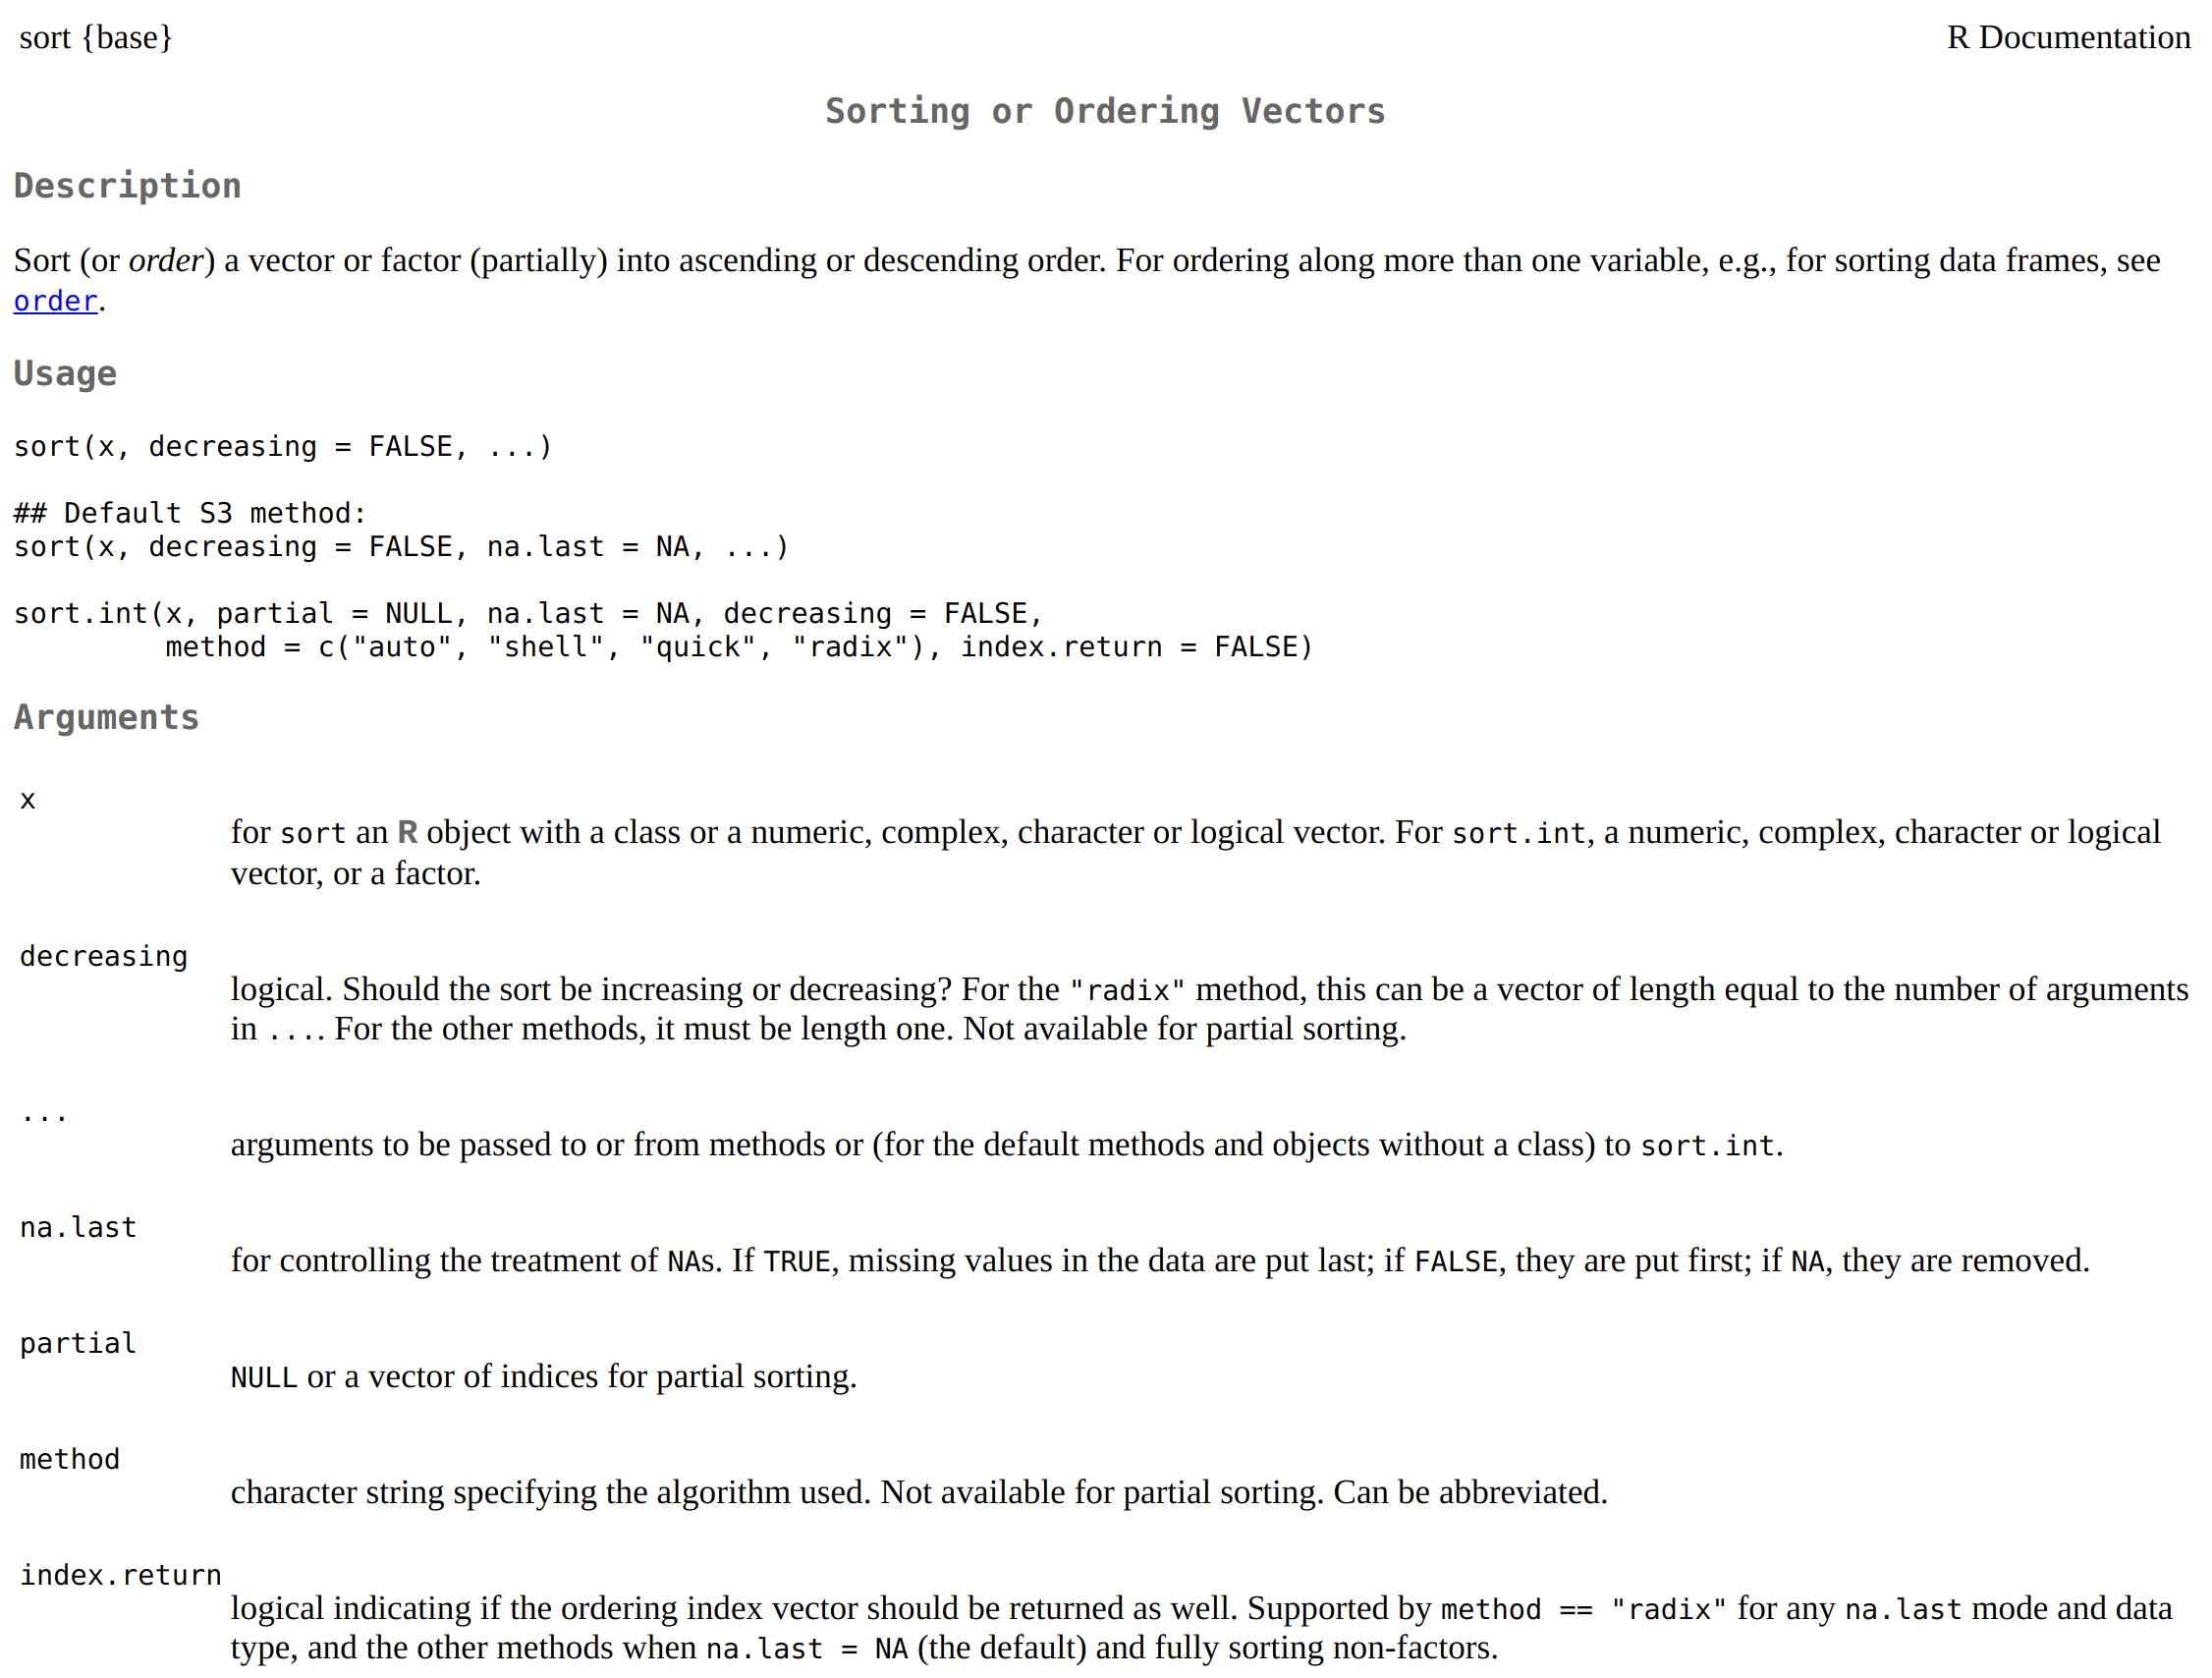
\includegraphics[width=1\linewidth]{images/sort-documentation} \end{center}

There's \emph{a ton} of information here, but all we're interested in at the moment is the order in which we need to pass arguments to \texttt{sort()}, which we can find in the \textbf{Arguments} section.

\hypertarget{missingness-and-nothingness}{%
\section{Missingness and Nothingness}\label{missingness-and-nothingness}}

\hypertarget{na}{%
\subsection{\texorpdfstring{\texttt{NA}}{NA}}\label{na}}

You may have noticed the \texttt{na.last} argument in \texttt{sort()}'s documentation. R can represent nothingness with \texttt{NULL} (same as \texttt{null} or \texttt{None} in other languages), but it can also represent \emph{unknown} or \emph{missing} values with \texttt{NA}.

\begin{Shaded}
\begin{Highlighting}[]
\NormalTok{unsorted\_numbers\_with\_nas \textless{}{-}}\StringTok{ }\KeywordTok{c}\NormalTok{(}\DecValTok{3}\NormalTok{, }\DecValTok{2}\NormalTok{, }\DecValTok{10}\NormalTok{, }\DecValTok{8}\NormalTok{, }\OtherTok{NA}\NormalTok{, }\DecValTok{1}\NormalTok{, }\DecValTok{4}\NormalTok{, }\DecValTok{9}\NormalTok{, }\OtherTok{NA}\NormalTok{, }\DecValTok{6}\NormalTok{, }\DecValTok{5}\NormalTok{, }\DecValTok{7}\NormalTok{)}
\NormalTok{unsorted\_numbers\_with\_nas}
\CommentTok{\#\textgreater{}  [1]  3  2 10  8 NA  1  4  9 NA  6  5  7}
\end{Highlighting}
\end{Shaded}

\texttt{sort()}'s default behavior is \texttt{na.last\ =\ NA}, which simply removes any \texttt{NA}s.

\begin{Shaded}
\begin{Highlighting}[]
\KeywordTok{sort}\NormalTok{(unsorted\_numbers\_with\_nas)}
\CommentTok{\#\textgreater{}  [1]  1  2  3  4  5  6  7  8  9 10}
\end{Highlighting}
\end{Shaded}

If we want to keep \texttt{NA}s, we must specify whether \texttt{sort()} places them first or last.

\begin{Shaded}
\begin{Highlighting}[]
\KeywordTok{sort}\NormalTok{(unsorted\_numbers\_with\_nas, }\DataTypeTok{na.last =} \OtherTok{TRUE}\NormalTok{)}
\CommentTok{\#\textgreater{}  [1]  1  2  3  4  5  6  7  8  9 10 NA NA}
\KeywordTok{sort}\NormalTok{(unsorted\_numbers\_with\_nas, }\DataTypeTok{na.last =} \OtherTok{FALSE}\NormalTok{)}
\CommentTok{\#\textgreater{}  [1] NA NA  1  2  3  4  5  6  7  8  9 10}
\end{Highlighting}
\end{Shaded}

\hypertarget{null}{%
\subsection{\texorpdfstring{\texttt{NULL}}{NULL}}\label{null}}

For the moment, think of the difference between \texttt{NA} and \texttt{NULL} as being that \texttt{vector}s (like \texttt{unsorted\_numbers\_with\_nas}) can have \texttt{NA} values but they cannot have \texttt{NULL} values.

If we try to put \texttt{NULL} in a \texttt{vector}, it simply disappears.

\begin{Shaded}
\begin{Highlighting}[]
\KeywordTok{c}\NormalTok{(}\DecValTok{3}\NormalTok{, }\DecValTok{2}\NormalTok{, }\DecValTok{10}\NormalTok{, }\DecValTok{8}\NormalTok{, }\OtherTok{NULL}\NormalTok{, }\DecValTok{1}\NormalTok{, }\DecValTok{4}\NormalTok{, }\DecValTok{9}\NormalTok{, }\OtherTok{NULL}\NormalTok{, }\DecValTok{6}\NormalTok{, }\DecValTok{5}\NormalTok{, }\DecValTok{7}\NormalTok{)}
\CommentTok{\#\textgreater{}  [1]  3  2 10  8  1  4  9  6  5  7}
\end{Highlighting}
\end{Shaded}

But, how do we check if something is \texttt{NA} or \texttt{NULL}?

\hypertarget{predicate-functions}{%
\section{Predicate Functions}\label{predicate-functions}}

A \emph{predicate function} is a function that \texttt{return}s either \texttt{TRUE} or \texttt{FALSE} based on some condition the function is checking.

Predicate functions \emph{should} use a name that expresses this intent, such as \texttt{is\textless{}some\ condition\textgreater{}}, \texttt{any\textless{}some\ condition\textgreater{}()}, or \texttt{all\textless{}some\ condition\textgreater{}()}.

If we want check if something is \texttt{NULL}, we use \texttt{is.null()}.

\begin{Shaded}
\begin{Highlighting}[]
\KeywordTok{is.null}\NormalTok{(}\StringTok{"this string isn\textquotesingle{}t NULL!"}\NormalTok{)}
\CommentTok{\#\textgreater{} [1] FALSE}
\KeywordTok{is.null}\NormalTok{(}\OtherTok{NULL}\NormalTok{)}
\CommentTok{\#\textgreater{} [1] TRUE}
\end{Highlighting}
\end{Shaded}

R has \emph{many} built-in predicate functions, including ones to check the basic data types that we've already seen.

\begin{Shaded}
\begin{Highlighting}[]
\KeywordTok{is.double}\NormalTok{(}\DecValTok{1}\NormalTok{)}
\CommentTok{\#\textgreater{} [1] TRUE}
\KeywordTok{is.double}\NormalTok{(1L)}
\CommentTok{\#\textgreater{} [1] FALSE}

\NormalTok{vec\_dbl \textless{}{-}}\StringTok{ }\KeywordTok{c}\NormalTok{(}\DecValTok{8}\NormalTok{, }\DecValTok{6}\NormalTok{, }\DecValTok{7}\NormalTok{, }\DecValTok{5}\NormalTok{, }\DecValTok{3}\NormalTok{, }\DecValTok{0}\NormalTok{, }\DecValTok{9}\NormalTok{)}
\KeywordTok{is.double}\NormalTok{(vec\_dbl)}
\CommentTok{\#\textgreater{} [1] TRUE}

\KeywordTok{is.integer}\NormalTok{(}\DecValTok{1}\NormalTok{)}
\CommentTok{\#\textgreater{} [1] FALSE}
\KeywordTok{is.integer}\NormalTok{(1L)}
\CommentTok{\#\textgreater{} [1] TRUE}
\NormalTok{vec\_int \textless{}{-}}\StringTok{ }\DecValTok{1}\OperatorTok{:}\DecValTok{10}
\KeywordTok{is.integer}\NormalTok{(vec\_int)}
\CommentTok{\#\textgreater{} [1] TRUE}

\KeywordTok{is.character}\NormalTok{(}\FloatTok{3.14}\NormalTok{)}
\CommentTok{\#\textgreater{} [1] FALSE}
\KeywordTok{is.character}\NormalTok{(}\StringTok{"is it though?"}\NormalTok{)}
\CommentTok{\#\textgreater{} [1] TRUE}
\KeywordTok{is.character}\NormalTok{(letters)}
\CommentTok{\#\textgreater{} [1] TRUE}

\KeywordTok{is.logical}\NormalTok{(}\StringTok{"the year 2020"}\NormalTok{)}
\CommentTok{\#\textgreater{} [1] FALSE}
\KeywordTok{is.logical}\NormalTok{(}\OtherTok{TRUE}\NormalTok{)}
\CommentTok{\#\textgreater{} [1] TRUE}
\KeywordTok{is.logical}\NormalTok{(}\OtherTok{FALSE}\NormalTok{)}
\CommentTok{\#\textgreater{} [1] TRUE}
\NormalTok{vec\_lgl \textless{}{-}}\StringTok{ }\KeywordTok{c}\NormalTok{(}\OtherTok{TRUE}\NormalTok{, }\OtherTok{FALSE}\NormalTok{, }\OtherTok{TRUE}\NormalTok{)}
\KeywordTok{is.logical}\NormalTok{(vec\_lgl)}
\CommentTok{\#\textgreater{} [1] TRUE}
\end{Highlighting}
\end{Shaded}

Similar to \texttt{is.null()}, there's \texttt{is.na()}.

\begin{Shaded}
\begin{Highlighting}[]
\KeywordTok{is.na}\NormalTok{(}\StringTok{"not NA!"}\NormalTok{)}
\CommentTok{\#\textgreater{} [1] FALSE}
\KeywordTok{is.na}\NormalTok{(}\OtherTok{NA}\NormalTok{)}
\CommentTok{\#\textgreater{} [1] TRUE}
\end{Highlighting}
\end{Shaded}

Recall our variable \texttt{unsorted\_numbers\_with\_nas}.

\begin{Shaded}
\begin{Highlighting}[]
\NormalTok{unsorted\_numbers\_with\_nas}
\CommentTok{\#\textgreater{}  [1]  3  2 10  8 NA  1  4  9 NA  6  5  7}
\end{Highlighting}
\end{Shaded}

Consider the following:

\begin{itemize}
\tightlist
\item
  The predicate functions we've seen so far \texttt{return} either \texttt{TRUE} or \texttt{FALSE}.
\item
  \texttt{vector}s can contain both \texttt{NA} \emph{and} non-\texttt{NA} values.
\end{itemize}

Can you guess what \texttt{is.na()} \texttt{return}s?

\begin{Shaded}
\begin{Highlighting}[]
\KeywordTok{is.na}\NormalTok{(unsorted\_numbers\_with\_nas)}
\CommentTok{\#\textgreater{}  [1] FALSE FALSE FALSE FALSE  TRUE FALSE FALSE FALSE  TRUE FALSE FALSE FALSE}
\end{Highlighting}
\end{Shaded}

\begin{center}
\includegraphics[width=1\linewidth]{images/the-what} \end{center}

We'll discuss accessing a \texttt{vector}'s individual elements later, but \texttt{is.na()} is what we call a \emph{vectorized} function: a function that takes \texttt{vector} argument and operates on every element simultaneously.

\hypertarget{vectorized-functions}{%
\section{Vectorized Functions}\label{vectorized-functions}}

As high-speed R coders, we should prefer \texttt{vector}ized solutions whenever possible as they're not only idiomatic (and thus easy for other R users to understand), but they're typically several orders of magnitude faster than other solutions.

While R isn't the fastest language out there, complaints about its speed usually come from poor code, including code that ``speaks'' R with a C or Python accent.

The simplest way to wrap our heads around \texttt{vector}ized operations is with math. let's first make a \texttt{vector} with five \texttt{0}s in it.

We could do that like the following:

\begin{Shaded}
\begin{Highlighting}[]
\KeywordTok{c}\NormalTok{(}\DecValTok{0}\NormalTok{, }\DecValTok{0}\NormalTok{, }\DecValTok{0}\NormalTok{, }\DecValTok{0}\NormalTok{, }\DecValTok{0}\NormalTok{)}
\CommentTok{\#\textgreater{} [1] 0 0 0 0 0}
\end{Highlighting}
\end{Shaded}

But, good coders are \emph{lazy} and want to (correctly) automate everything they can. With that in mind, let's \texttt{rep()}eat \texttt{0} \texttt{5} times.

\begin{Shaded}
\begin{Highlighting}[]
\NormalTok{zeros \textless{}{-}}\StringTok{ }\KeywordTok{rep}\NormalTok{(}\DecValTok{0}\NormalTok{, }\DataTypeTok{length =} \DecValTok{5}\NormalTok{)}
\NormalTok{zeros}
\CommentTok{\#\textgreater{} [1] 0 0 0 0 0}
\end{Highlighting}
\end{Shaded}

For our purposes, the term \emph{scalar} refers to an object that is a single value.

If we want to add \texttt{1} (a scalar) to every element of \texttt{zeros}, we can run \texttt{zeros\ +\ 1} or \texttt{1\ +\ zeros}:

\begin{Shaded}
\begin{Highlighting}[]
\NormalTok{zeros }\OperatorTok{+}\StringTok{ }\DecValTok{1}
\CommentTok{\#\textgreater{} [1] 1 1 1 1 1}
\end{Highlighting}
\end{Shaded}

R knows that \texttt{1} is a single value (and assumes we know what we're doing) and performs the operation (\texttt{+}) between it and every element of \texttt{zeros}. In R-speak, we refer to this behavior as \emph{recycling}.

Let's see what happens when we add \texttt{zeros} and a \texttt{vector} containing two elements.

\begin{Shaded}
\begin{Highlighting}[]
\NormalTok{two\_threes \textless{}{-}}\StringTok{ }\KeywordTok{c}\NormalTok{(}\DecValTok{3}\NormalTok{, }\DecValTok{3}\NormalTok{)}

\NormalTok{zeros }\OperatorTok{+}\StringTok{ }\NormalTok{two\_threes}
\CommentTok{\#\textgreater{} Warning in zeros + two\_threes: longer object length is not a multiple of shorter object length}
\CommentTok{\#\textgreater{} [1] 3 3 3 3 3}
\end{Highlighting}
\end{Shaded}

That's probably not what you expected and R gives us a \texttt{warning()} to tell us something seems wrong.

R let's us get away with a lot of things it shouldn't, which includes

\cleardoublepage

\hypertarget{part-day-2}{%
\part{Day 2}\label{part-day-2}}

\hypertarget{tabular-data}{%
\chapter{Tabular Data}\label{tabular-data}}

\begin{itemize}
\tightlist
\item
  Aliases:

  \begin{itemize}
  \tightlist
  \item
    Tabular files
  \item
    Flat
  \item
    Delimited
  \end{itemize}
\item
  Includes:

  \begin{itemize}
  \tightlist
  \item
    Comma-Separated Value (.csv)
  \item
    Tab-Separated Value (.tsv)
  \end{itemize}
\end{itemize}

\hypertarget{basics}{%
\section{Basics}\label{basics}}

\begin{Shaded}
\begin{Highlighting}[]
\KeywordTok{library}\NormalTok{(readr)}
\end{Highlighting}
\end{Shaded}

Here's some example data, modified from \url{http://www.gapminder.org/data/}

\begin{verbatim}
country,continent,year,lifeExp,pop,gdpPercap       # header/column names, separated by commas
Afghanistan,Asia,1952,28.801,8425333,779.4453145
Afghanistan,Asia,1957,30.332,9240934,820.8530296   # comma-separated values
Afghanistan,Asia,1962,31.997,10267083,853.10071
Afghanistan,Asia,1967,34.02,11537966,836.1971382
Afghanistan,Asia,1972,36.088,13079460,739.9811058
Afghanistan,Asia,1977,38.438,14880372,786.11336
Afghanistan,Asia,1982,39.854,12881816,978.0114388
Afghanistan,Asia,1987,40.822,13867957,852.3959448
\end{verbatim}

\begin{Shaded}
\begin{Highlighting}[]
\NormalTok{csv\_text \textless{}{-}}\StringTok{ }
\StringTok{\textquotesingle{}country,continent,year,lifeExp,pop,gdpPercap     }
\StringTok{Afghanistan,Asia,1952,28.801,8425333,779.4453145}
\StringTok{Afghanistan,Asia,1957,30.332,9240934,820.8530296}
\StringTok{Afghanistan,Asia,1962,31.997,10267083,853.10071}
\StringTok{Afghanistan,Asia,1967,34.02,11537966,836.1971382}
\StringTok{Afghanistan,Asia,1972,36.088,13079460,739.9811058}
\StringTok{Afghanistan,Asia,1977,38.438,14880372,786.11336}
\StringTok{Afghanistan,Asia,1982,39.854,12881816,978.0114388}
\StringTok{Afghanistan,Asia,1987,40.822,13867957,852.3959448\textquotesingle{}}

\NormalTok{csv\_file \textless{}{-}}\StringTok{ }\KeywordTok{tempfile}\NormalTok{(}\DataTypeTok{fileext =} \StringTok{".csv"}\NormalTok{)      }
\NormalTok{csv\_file }\CommentTok{\# a temporary file path}
\CommentTok{\#\textgreater{} [1] "/tmp/RtmpuxJjlO/file386534d96861.csv"}
\KeywordTok{writeLines}\NormalTok{(}\DataTypeTok{text =}\NormalTok{ csv\_text, }\DataTypeTok{con =}\NormalTok{ csv\_file) }\CommentTok{\# write \textasciigrave{}csv\_text\textasciigrave{} to \textasciigrave{}csv\_file\textasciigrave{}}
\end{Highlighting}
\end{Shaded}

\begin{Shaded}
\begin{Highlighting}[]
\KeywordTok{read\_csv}\NormalTok{(}\DataTypeTok{file =}\NormalTok{ csv\_file)}
\CommentTok{\#\textgreater{} Parsed with column specification:}
\CommentTok{\#\textgreater{} cols(}
\CommentTok{\#\textgreater{}   country = col\_character(),}
\CommentTok{\#\textgreater{}   continent = col\_character(),}
\CommentTok{\#\textgreater{}   year = col\_double(),}
\CommentTok{\#\textgreater{}   lifeExp = col\_double(),}
\CommentTok{\#\textgreater{}   pop = col\_double(),}
\CommentTok{\#\textgreater{}   gdpPercap = col\_double()}
\CommentTok{\#\textgreater{} )}
\CommentTok{\#\textgreater{} \# A tibble: 8 x 6}
\CommentTok{\#\textgreater{}   country     continent  year lifeExp      pop gdpPercap}
\CommentTok{\#\textgreater{}   \textless{}chr\textgreater{}       \textless{}chr\textgreater{}     \textless{}dbl\textgreater{}   \textless{}dbl\textgreater{}    \textless{}dbl\textgreater{}     \textless{}dbl\textgreater{}}
\CommentTok{\#\textgreater{} 1 Afghanistan Asia       1952    28.8  8425333      779.}
\CommentTok{\#\textgreater{} 2 Afghanistan Asia       1957    30.3  9240934      821.}
\CommentTok{\#\textgreater{} 3 Afghanistan Asia       1962    32.0 10267083      853.}
\CommentTok{\#\textgreater{} 4 Afghanistan Asia       1967    34.0 11537966      836.}
\CommentTok{\#\textgreater{} 5 Afghanistan Asia       1972    36.1 13079460      740.}
\CommentTok{\#\textgreater{} 6 Afghanistan Asia       1977    38.4 14880372      786.}
\CommentTok{\#\textgreater{} 7 Afghanistan Asia       1982    39.9 12881816      978.}
\CommentTok{\#\textgreater{} 8 Afghanistan Asia       1987    40.8 13867957      852.}
\end{Highlighting}
\end{Shaded}

You may encounter Tab-Delimited data where values are separated by \texttt{\textbackslash{}t} instead of \texttt{,}. Instead of \texttt{readr::read\_csv()}, we can use \texttt{readr::read\_tsv()}.

\begin{Shaded}
\begin{Highlighting}[]
\NormalTok{tsv\_text \textless{}{-}}\StringTok{ }
\StringTok{\textquotesingle{}country}\CharTok{\textbackslash{}t}\StringTok{continent}\CharTok{\textbackslash{}t}\StringTok{year}\CharTok{\textbackslash{}t}\StringTok{lifeExp}\CharTok{\textbackslash{}t}\StringTok{pop}\CharTok{\textbackslash{}t}\StringTok{gdpPercap     }
\StringTok{Afghanistan}\CharTok{\textbackslash{}t}\StringTok{Asia}\CharTok{\textbackslash{}t}\StringTok{1952}\CharTok{\textbackslash{}t}\StringTok{28.801}\CharTok{\textbackslash{}t}\StringTok{8425333}\CharTok{\textbackslash{}t}\StringTok{779.4453145}
\StringTok{Afghanistan}\CharTok{\textbackslash{}t}\StringTok{Asia}\CharTok{\textbackslash{}t}\StringTok{1957}\CharTok{\textbackslash{}t}\StringTok{30.332}\CharTok{\textbackslash{}t}\StringTok{9240934}\CharTok{\textbackslash{}t}\StringTok{820.8530296}
\StringTok{Afghanistan}\CharTok{\textbackslash{}t}\StringTok{Asia}\CharTok{\textbackslash{}t}\StringTok{1962}\CharTok{\textbackslash{}t}\StringTok{31.997}\CharTok{\textbackslash{}t}\StringTok{10267083}\CharTok{\textbackslash{}t}\StringTok{853.10071}
\StringTok{Afghanistan}\CharTok{\textbackslash{}t}\StringTok{Asia}\CharTok{\textbackslash{}t}\StringTok{1967}\CharTok{\textbackslash{}t}\StringTok{34.02}\CharTok{\textbackslash{}t}\StringTok{11537966}\CharTok{\textbackslash{}t}\StringTok{836.1971382}
\StringTok{Afghanistan}\CharTok{\textbackslash{}t}\StringTok{Asia}\CharTok{\textbackslash{}t}\StringTok{1972}\CharTok{\textbackslash{}t}\StringTok{36.088}\CharTok{\textbackslash{}t}\StringTok{13079460}\CharTok{\textbackslash{}t}\StringTok{739.9811058}
\StringTok{Afghanistan}\CharTok{\textbackslash{}t}\StringTok{Asia}\CharTok{\textbackslash{}t}\StringTok{1977}\CharTok{\textbackslash{}t}\StringTok{38.438}\CharTok{\textbackslash{}t}\StringTok{14880372}\CharTok{\textbackslash{}t}\StringTok{786.11336}
\StringTok{Afghanistan}\CharTok{\textbackslash{}t}\StringTok{Asia}\CharTok{\textbackslash{}t}\StringTok{1982}\CharTok{\textbackslash{}t}\StringTok{39.854}\CharTok{\textbackslash{}t}\StringTok{12881816}\CharTok{\textbackslash{}t}\StringTok{978.0114388}
\StringTok{Afghanistan}\CharTok{\textbackslash{}t}\StringTok{Asia}\CharTok{\textbackslash{}t}\StringTok{1987}\CharTok{\textbackslash{}t}\StringTok{40.822}\CharTok{\textbackslash{}t}\StringTok{13867957}\CharTok{\textbackslash{}t}\StringTok{852.3959448\textquotesingle{}}

\NormalTok{tsv\_file \textless{}{-}}\StringTok{ }\KeywordTok{tempfile}\NormalTok{(}\DataTypeTok{fileext =} \StringTok{".tsv"}\NormalTok{)}
\KeywordTok{writeLines}\NormalTok{(}\DataTypeTok{text =}\NormalTok{ tsv\_text, }\DataTypeTok{con =}\NormalTok{ tsv\_file)}
\end{Highlighting}
\end{Shaded}

\begin{Shaded}
\begin{Highlighting}[]
\KeywordTok{read\_tsv}\NormalTok{(}\DataTypeTok{file =}\NormalTok{ tsv\_file)}
\CommentTok{\#\textgreater{} Parsed with column specification:}
\CommentTok{\#\textgreater{} cols(}
\CommentTok{\#\textgreater{}   country = col\_character(),}
\CommentTok{\#\textgreater{}   continent = col\_character(),}
\CommentTok{\#\textgreater{}   year = col\_double(),}
\CommentTok{\#\textgreater{}   lifeExp = col\_double(),}
\CommentTok{\#\textgreater{}   pop = col\_double(),}
\CommentTok{\#\textgreater{}   gdpPercap = col\_double()}
\CommentTok{\#\textgreater{} )}
\CommentTok{\#\textgreater{} \# A tibble: 8 x 6}
\CommentTok{\#\textgreater{}   country     continent  year lifeExp      pop gdpPercap}
\CommentTok{\#\textgreater{}   \textless{}chr\textgreater{}       \textless{}chr\textgreater{}     \textless{}dbl\textgreater{}   \textless{}dbl\textgreater{}    \textless{}dbl\textgreater{}     \textless{}dbl\textgreater{}}
\CommentTok{\#\textgreater{} 1 Afghanistan Asia       1952    28.8  8425333      779.}
\CommentTok{\#\textgreater{} 2 Afghanistan Asia       1957    30.3  9240934      821.}
\CommentTok{\#\textgreater{} 3 Afghanistan Asia       1962    32.0 10267083      853.}
\CommentTok{\#\textgreater{} 4 Afghanistan Asia       1967    34.0 11537966      836.}
\CommentTok{\#\textgreater{} 5 Afghanistan Asia       1972    36.1 13079460      740.}
\CommentTok{\#\textgreater{} 6 Afghanistan Asia       1977    38.4 14880372      786.}
\CommentTok{\#\textgreater{} 7 Afghanistan Asia       1982    39.9 12881816      978.}
\CommentTok{\#\textgreater{} 8 Afghanistan Asia       1987    40.8 13867957      852.}
\end{Highlighting}
\end{Shaded}

If we find ourselves reading delmited data that uses something other than \texttt{\textbackslash{}t} or \texttt{,} to separate values, we can use \texttt{readr::read\_delim()}.

\begin{Shaded}
\begin{Highlighting}[]
\NormalTok{pipe\_separated\_values\_text \textless{}{-}}\StringTok{ }
\StringTok{\textquotesingle{}country|continent|year|lifeExp|pop|gdpPercap     }
\StringTok{Afghanistan|Asia|1952|28.801|8425333|779.4453145}
\StringTok{Afghanistan|Asia|1957|30.332|9240934|820.8530296}
\StringTok{Afghanistan|Asia|1962|31.997|10267083|853.10071}
\StringTok{Afghanistan|Asia|1967|34.02|11537966|836.1971382}
\StringTok{Afghanistan|Asia|1972|36.088|13079460|739.9811058}
\StringTok{Afghanistan|Asia|1977|38.438|14880372|786.11336}
\StringTok{Afghanistan|Asia|1982|39.854|12881816|978.0114388}
\StringTok{Afghanistan|Asia|1987|40.822|13867957|852.3959448\textquotesingle{}}

\NormalTok{psv\_file \textless{}{-}}\StringTok{ }\KeywordTok{tempfile}\NormalTok{(}\DataTypeTok{fileext =} \StringTok{".tsv"}\NormalTok{)}
\KeywordTok{writeLines}\NormalTok{(}\DataTypeTok{text =}\NormalTok{ pipe\_separated\_values\_text, }\DataTypeTok{con =}\NormalTok{ psv\_file)}
\end{Highlighting}
\end{Shaded}

\begin{Shaded}
\begin{Highlighting}[]
\KeywordTok{read\_delim}\NormalTok{(}\DataTypeTok{file =}\NormalTok{ psv\_file, }\DataTypeTok{delim =} \StringTok{"|"}\NormalTok{)}
\CommentTok{\#\textgreater{} Parsed with column specification:}
\CommentTok{\#\textgreater{} cols(}
\CommentTok{\#\textgreater{}   country = col\_character(),}
\CommentTok{\#\textgreater{}   continent = col\_character(),}
\CommentTok{\#\textgreater{}   year = col\_double(),}
\CommentTok{\#\textgreater{}   lifeExp = col\_double(),}
\CommentTok{\#\textgreater{}   pop = col\_double(),}
\CommentTok{\#\textgreater{}   \textasciigrave{}gdpPercap     \textasciigrave{} = col\_double()}
\CommentTok{\#\textgreater{} )}
\CommentTok{\#\textgreater{} \# A tibble: 8 x 6}
\CommentTok{\#\textgreater{}   country     continent  year lifeExp      pop \textasciigrave{}gdpPercap     \textasciigrave{}}
\CommentTok{\#\textgreater{}   \textless{}chr\textgreater{}       \textless{}chr\textgreater{}     \textless{}dbl\textgreater{}   \textless{}dbl\textgreater{}    \textless{}dbl\textgreater{}            \textless{}dbl\textgreater{}}
\CommentTok{\#\textgreater{} 1 Afghanistan Asia       1952    28.8  8425333             779.}
\CommentTok{\#\textgreater{} 2 Afghanistan Asia       1957    30.3  9240934             821.}
\CommentTok{\#\textgreater{} 3 Afghanistan Asia       1962    32.0 10267083             853.}
\CommentTok{\#\textgreater{} 4 Afghanistan Asia       1967    34.0 11537966             836.}
\CommentTok{\#\textgreater{} 5 Afghanistan Asia       1972    36.1 13079460             740.}
\CommentTok{\#\textgreater{} 6 Afghanistan Asia       1977    38.4 14880372             786.}
\CommentTok{\#\textgreater{} 7 Afghanistan Asia       1982    39.9 12881816             978.}
\CommentTok{\#\textgreater{} 8 Afghanistan Asia       1987    40.8 13867957             852.}
\end{Highlighting}
\end{Shaded}

\begin{verbatim}
country,continent,year,lifeExp,pop,gdpPercap       # header/column names
Afghanistan,Asia,1952,28.801,8425333,779.4453145
Afghanistan,Asia,1957,30.332,9240934,820.8530296
Afghanistan,Asia,1962,31.997,10267083,853.10071
Afghanistan,Asia,1967,34.02,11537966,836.1971382
Afghanistan,Asia,1972,36.088,13079460,739.9811058
Afghanistan,Asia,1977,38.438,14880372,786.11336
Afghanistan,Asia,1982,39.854,12881816,978.0114388
Afghanistan,Asia,1987,40.822,13867957,852.3959448
Afghanistan,,,N/A,,                                # notice that we're missing values
\end{verbatim}

\begin{Shaded}
\begin{Highlighting}[]
\NormalTok{csv\_text \textless{}{-}}\StringTok{ }
\StringTok{\textquotesingle{}country,continent,year,lifeExp,pop,gdpPercap}
\StringTok{Afghanistan,Asia,1952,28.801,8425333,779.4453145}
\StringTok{Afghanistan,Asia,1957,30.332,9240934,820.8530296}
\StringTok{Afghanistan,Asia,1962,31.997,10267083,853.10071}
\StringTok{Afghanistan,Asia,1967,34.02,11537966,836.1971382}
\StringTok{Afghanistan,Asia,1972,36.088,13079460,739.9811058}
\StringTok{Afghanistan,Asia,1977,38.438,14880372,786.11336}
\StringTok{Afghanistan,Asia,1982,39.854,12881816,978.0114388}
\StringTok{Afghanistan,Asia,1987,40.822,13867957,852.3959448}
\StringTok{Afghanistan,,,N/A,,\textquotesingle{}}

\NormalTok{csv\_file \textless{}{-}}\StringTok{ }\KeywordTok{tempfile}\NormalTok{(}\DataTypeTok{fileext =} \StringTok{".csv"}\NormalTok{)}
\KeywordTok{writeLines}\NormalTok{(}\DataTypeTok{text =}\NormalTok{ csv\_text, }\DataTypeTok{con =}\NormalTok{ csv\_file)}
\end{Highlighting}
\end{Shaded}

\hypertarget{common-pitfalls}{%
\section{Common Pitfalls}\label{common-pitfalls}}

\hypertarget{incorrect-column-types}{%
\subsection{Incorrect Column Types}\label{incorrect-column-types}}

\begin{Shaded}
\begin{Highlighting}[]
\NormalTok{data\_frame\_from\_csv \textless{}{-}}\StringTok{ }\KeywordTok{read\_csv}\NormalTok{(}\DataTypeTok{file =}\NormalTok{ csv\_file)}
\CommentTok{\#\textgreater{} Parsed with column specification:}
\CommentTok{\#\textgreater{} cols(}
\CommentTok{\#\textgreater{}   country = col\_character(),}
\CommentTok{\#\textgreater{}   continent = col\_character(),}
\CommentTok{\#\textgreater{}   year = col\_double(),}
\CommentTok{\#\textgreater{}   lifeExp = col\_character(),}
\CommentTok{\#\textgreater{}   pop = col\_double(),}
\CommentTok{\#\textgreater{}   gdpPercap = col\_double()}
\CommentTok{\#\textgreater{} )}
\NormalTok{data\_frame\_from\_csv}
\CommentTok{\#\textgreater{} \# A tibble: 9 x 6}
\CommentTok{\#\textgreater{}   country     continent  year lifeExp      pop gdpPercap}
\CommentTok{\#\textgreater{}   \textless{}chr\textgreater{}       \textless{}chr\textgreater{}     \textless{}dbl\textgreater{} \textless{}chr\textgreater{}      \textless{}dbl\textgreater{}     \textless{}dbl\textgreater{}}
\CommentTok{\#\textgreater{} 1 Afghanistan Asia       1952 28.801   8425333      779.}
\CommentTok{\#\textgreater{} 2 Afghanistan Asia       1957 30.332   9240934      821.}
\CommentTok{\#\textgreater{} 3 Afghanistan Asia       1962 31.997  10267083      853.}
\CommentTok{\#\textgreater{} 4 Afghanistan Asia       1967 34.02   11537966      836.}
\CommentTok{\#\textgreater{} 5 Afghanistan Asia       1972 36.088  13079460      740.}
\CommentTok{\#\textgreater{} 6 Afghanistan Asia       1977 38.438  14880372      786.}
\CommentTok{\#\textgreater{} 7 Afghanistan Asia       1982 39.854  12881816      978.}
\CommentTok{\#\textgreater{} 8 Afghanistan Asia       1987 40.822  13867957      852.}
\CommentTok{\#\textgreater{} 9 Afghanistan \textless{}NA\textgreater{}         NA N/A           NA       NA}
\end{Highlighting}
\end{Shaded}

Notice that our \texttt{year} column says \texttt{\textless{}dbl\textgreater{}}, referring to it being of type \texttt{double}, yet all of our \texttt{year} values are whole numbers.

\begin{Shaded}
\begin{Highlighting}[]
\KeywordTok{typeof}\NormalTok{(data\_frame\_from\_csv}\OperatorTok{$}\NormalTok{year)}
\CommentTok{\#\textgreater{} [1] "double"}
\NormalTok{data\_frame\_from\_csv}\OperatorTok{$}\NormalTok{year}
\CommentTok{\#\textgreater{} [1] 1952 1957 1962 1967 1972 1977 1982 1987   NA}
\end{Highlighting}
\end{Shaded}

We also have \texttt{"N/A"} in our \texttt{lifeExp} column, forcing R to interpret all \texttt{lifeExp} values as \texttt{character}s (\texttt{\textless{}chr\textgreater{}}).

\begin{Shaded}
\begin{Highlighting}[]
\KeywordTok{typeof}\NormalTok{(data\_frame\_from\_csv}\OperatorTok{$}\NormalTok{lifeExp)}
\CommentTok{\#\textgreater{} [1] "character"}
\NormalTok{data\_frame\_from\_csv}\OperatorTok{$}\NormalTok{lifeExp}
\CommentTok{\#\textgreater{} [1] "28.801" "30.332" "31.997" "34.02"  "36.088" "38.438" "39.854" "40.822" "N/A"}
\end{Highlighting}
\end{Shaded}

\hypertarget{solution}{%
\subsubsection{Solution}\label{solution}}

\begin{Shaded}
\begin{Highlighting}[]
\KeywordTok{read\_csv}\NormalTok{(}
  \DataTypeTok{file =}\NormalTok{ csv\_file,}
  \DataTypeTok{col\_types =} \KeywordTok{cols}\NormalTok{(}
    \DataTypeTok{country =} \KeywordTok{col\_character}\NormalTok{(),}
    \DataTypeTok{continent =} \KeywordTok{col\_character}\NormalTok{(),}
    \DataTypeTok{year =} \KeywordTok{col\_integer}\NormalTok{(),        }\CommentTok{\# read \textasciigrave{}year\textasciigrave{} as \textasciigrave{}integer\textasciigrave{}}
    \DataTypeTok{lifeExp =} \KeywordTok{col\_double}\NormalTok{(),      }\CommentTok{\# read \textasciigrave{}lifeExp\textasciigrave{} as \textasciigrave{}double\textasciigrave{}}
    \DataTypeTok{pop =} \KeywordTok{col\_double}\NormalTok{(),}
    \DataTypeTok{gdpPercap =} \KeywordTok{col\_double}\NormalTok{()}
\NormalTok{  ),}
  \DataTypeTok{na =} \KeywordTok{c}\NormalTok{(}\StringTok{""}\NormalTok{, }\StringTok{"N/A"}\NormalTok{)              }\CommentTok{\# be explicit about how \textasciigrave{}csv\_file\textasciigrave{} represents missing values}
\NormalTok{)}
\CommentTok{\#\textgreater{} \# A tibble: 9 x 6}
\CommentTok{\#\textgreater{}   country     continent  year lifeExp      pop gdpPercap}
\CommentTok{\#\textgreater{}   \textless{}chr\textgreater{}       \textless{}chr\textgreater{}     \textless{}int\textgreater{}   \textless{}dbl\textgreater{}    \textless{}dbl\textgreater{}     \textless{}dbl\textgreater{}}
\CommentTok{\#\textgreater{} 1 Afghanistan Asia       1952    28.8  8425333      779.}
\CommentTok{\#\textgreater{} 2 Afghanistan Asia       1957    30.3  9240934      821.}
\CommentTok{\#\textgreater{} 3 Afghanistan Asia       1962    32.0 10267083      853.}
\CommentTok{\#\textgreater{} 4 Afghanistan Asia       1967    34.0 11537966      836.}
\CommentTok{\#\textgreater{} 5 Afghanistan Asia       1972    36.1 13079460      740.}
\CommentTok{\#\textgreater{} 6 Afghanistan Asia       1977    38.4 14880372      786.}
\CommentTok{\#\textgreater{} 7 Afghanistan Asia       1982    39.9 12881816      978.}
\CommentTok{\#\textgreater{} 8 Afghanistan Asia       1987    40.8 13867957      852.}
\CommentTok{\#\textgreater{} 9 Afghanistan \textless{}NA\textgreater{}         NA    NA         NA       NA}
\end{Highlighting}
\end{Shaded}

\hypertarget{manipulating-data-frames}{%
\chapter{Manipulating Data Frames}\label{manipulating-data-frames}}

\begin{Shaded}
\begin{Highlighting}[]
\KeywordTok{library}\NormalTok{(tidyverse, }\DataTypeTok{warn.conflicts =} \OtherTok{FALSE}\NormalTok{)}
\CommentTok{\#\textgreater{} {-}{-} Attaching packages {-}{-}{-}{-}{-}{-}{-}{-}{-}{-}{-}{-}{-}{-}{-}{-}{-}{-}{-}{-}{-}{-}{-}{-}{-}{-}{-}{-}{-}{-}{-}{-}{-}{-}{-}{-}{-}{-}{-}{-}{-}{-}{-}{-}{-}{-}{-}{-}{-}{-}{-}{-}{-}{-}{-}{-}{-}{-}{-}{-}{-}{-}{-}{-} tidyverse 1.3.0 {-}{-}}
\CommentTok{\#\textgreater{} v ggplot2 3.3.2     v purrr   0.3.4}
\CommentTok{\#\textgreater{} v tibble  3.0.3     v dplyr   1.0.2}
\CommentTok{\#\textgreater{} v tidyr   1.1.2     v stringr 1.4.0}
\CommentTok{\#\textgreater{} v readr   1.3.1     v forcats 0.5.0}
\CommentTok{\#\textgreater{} {-}{-} Conflicts {-}{-}{-}{-}{-}{-}{-}{-}{-}{-}{-}{-}{-}{-}{-}{-}{-}{-}{-}{-}{-}{-}{-}{-}{-}{-}{-}{-}{-}{-}{-}{-}{-}{-}{-}{-}{-}{-}{-}{-}{-}{-}{-}{-}{-}{-}{-}{-}{-}{-}{-}{-}{-}{-}{-}{-}{-}{-}{-}{-}{-}{-}{-}{-}{-}{-}{-} tidyverse\_conflicts() {-}{-}}
\CommentTok{\#\textgreater{} x dplyr::filter() masks stats::filter()}
\CommentTok{\#\textgreater{} x dplyr::lag()    masks stats::lag()}

\NormalTok{df \textless{}{-}}\StringTok{ }\KeywordTok{tibble}\NormalTok{(}
  \DataTypeTok{group =} \KeywordTok{c}\NormalTok{(}\StringTok{"a"}\NormalTok{, }\StringTok{"a"}\NormalTok{, }\StringTok{"b"}\NormalTok{, }\StringTok{"b"}\NormalTok{, }\StringTok{"b"}\NormalTok{),}
  \DataTypeTok{a =} \KeywordTok{c}\NormalTok{(}\DecValTok{1}\NormalTok{, }\DecValTok{4}\NormalTok{, }\OtherTok{NA}\NormalTok{, }\DecValTok{3}\NormalTok{, }\DecValTok{5}\NormalTok{),}
  \DataTypeTok{b =} \KeywordTok{c}\NormalTok{(}\DecValTok{9}\NormalTok{, }\OtherTok{NA}\NormalTok{, }\DecValTok{8}\NormalTok{, }\DecValTok{10}\NormalTok{, }\DecValTok{7}\NormalTok{),}
  \DataTypeTok{c =} \KeywordTok{c}\NormalTok{(}\OtherTok{TRUE}\NormalTok{, }\OtherTok{FALSE}\NormalTok{, }\OtherTok{NA}\NormalTok{, }\OtherTok{FALSE}\NormalTok{, }\OtherTok{TRUE}\NormalTok{),}
  \DataTypeTok{d =} \KeywordTok{c}\NormalTok{(LETTERS[}\DecValTok{1}\OperatorTok{:}\DecValTok{3}\NormalTok{], }\OtherTok{NA}\NormalTok{, LETTERS[[}\DecValTok{5}\NormalTok{]]),}
  \DataTypeTok{e =} \KeywordTok{factor}\NormalTok{(}\DecValTok{1}\OperatorTok{:}\DecValTok{5}\NormalTok{, }\DataTypeTok{labels =} \KeywordTok{c}\NormalTok{(}\StringTok{"tiny"}\NormalTok{, }\StringTok{"small"}\NormalTok{, }\StringTok{"medium"}\NormalTok{, }\StringTok{"big"}\NormalTok{, }\StringTok{"huge"}\NormalTok{)),}
  \DataTypeTok{f\_col =} \KeywordTok{c}\NormalTok{(}\KeywordTok{as.Date}\NormalTok{(}\OtherTok{NA}\NormalTok{), }\KeywordTok{as.Date}\NormalTok{(}\StringTok{"2020{-}09{-}23"}\NormalTok{) }\OperatorTok{+}\StringTok{ }\KeywordTok{c}\NormalTok{(}\DecValTok{3}\NormalTok{, }\DecValTok{2}\NormalTok{, }\DecValTok{1}\NormalTok{, }\DecValTok{4}\NormalTok{)),}
  \DataTypeTok{g\_col =} \KeywordTok{c}\NormalTok{(}\KeywordTok{as.POSIXct}\NormalTok{(}\StringTok{"2020{-}09{-}23 00:00:00"}\NormalTok{) }\OperatorTok{+}\StringTok{ }\DecValTok{1}\OperatorTok{:}\DecValTok{4} \OperatorTok{*}\StringTok{ }\DecValTok{60} \OperatorTok{*}\StringTok{ }\DecValTok{60} \OperatorTok{*}\StringTok{ }\DecValTok{24} \OperatorTok{*}\StringTok{ }\FloatTok{1.1}\NormalTok{, }\OtherTok{NA}\NormalTok{),}
  \DataTypeTok{col\_h =} \KeywordTok{list}\NormalTok{(}\KeywordTok{c}\NormalTok{(}\DecValTok{1}\NormalTok{, }\DecValTok{10}\NormalTok{), }\KeywordTok{c}\NormalTok{(}\DecValTok{2}\NormalTok{, }\OtherTok{NA}\NormalTok{), }\KeywordTok{c}\NormalTok{(}\DecValTok{3}\NormalTok{, }\DecValTok{8}\NormalTok{), }\KeywordTok{c}\NormalTok{(}\DecValTok{4}\NormalTok{, }\DecValTok{7}\NormalTok{), }\KeywordTok{c}\NormalTok{(}\DecValTok{5}\NormalTok{, }\DecValTok{6}\NormalTok{)),}
  \DataTypeTok{col\_i =} \KeywordTok{list}\NormalTok{(}\OtherTok{NULL}\NormalTok{, pi, month.abb[}\DecValTok{6}\OperatorTok{:}\DecValTok{10}\NormalTok{], iris, }\KeywordTok{as.matrix}\NormalTok{(mtcars))}
\NormalTok{)}

\NormalTok{df}
\CommentTok{\#\textgreater{} \# A tibble: 5 x 10}
\CommentTok{\#\textgreater{}   group     a     b c     d     e      f\_col      g\_col               col\_h    col\_i           }
\CommentTok{\#\textgreater{}   \textless{}chr\textgreater{} \textless{}dbl\textgreater{} \textless{}dbl\textgreater{} \textless{}lgl\textgreater{} \textless{}chr\textgreater{} \textless{}fct\textgreater{}  \textless{}date\textgreater{}     \textless{}dttm\textgreater{}              \textless{}list\textgreater{}   \textless{}list\textgreater{}          }
\CommentTok{\#\textgreater{} 1 a         1     9 TRUE  A     tiny   NA         2020{-}09{-}24 02:24:00 \textless{}dbl [2\textasciitilde{} \textless{}NULL\textgreater{}          }
\CommentTok{\#\textgreater{} 2 a         4    NA FALSE B     small  2020{-}09{-}26 2020{-}09{-}25 04:48:00 \textless{}dbl [2\textasciitilde{} \textless{}dbl [1]\textgreater{}       }
\CommentTok{\#\textgreater{} 3 b        NA     8 NA    C     medium 2020{-}09{-}25 2020{-}09{-}26 07:12:00 \textless{}dbl [2\textasciitilde{} \textless{}chr [5]\textgreater{}       }
\CommentTok{\#\textgreater{} 4 b         3    10 FALSE \textless{}NA\textgreater{}  big    2020{-}09{-}24 2020{-}09{-}27 09:36:00 \textless{}dbl [2\textasciitilde{} \textless{}df[,5] [150 x \textasciitilde{}}
\CommentTok{\#\textgreater{} 5 b         5     7 TRUE  E     huge   2020{-}09{-}27 NA                  \textless{}dbl [2\textasciitilde{} \textless{}dbl[,11] [32 x\textasciitilde{}}
\KeywordTok{glimpse}\NormalTok{(df)}
\CommentTok{\#\textgreater{} Rows: 5}
\CommentTok{\#\textgreater{} Columns: 10}
\CommentTok{\#\textgreater{} $ group \textless{}chr\textgreater{} "a", "a", "b", "b", "b"}
\CommentTok{\#\textgreater{} $ a     \textless{}dbl\textgreater{} 1, 4, NA, 3, 5}
\CommentTok{\#\textgreater{} $ b     \textless{}dbl\textgreater{} 9, NA, 8, 10, 7}
\CommentTok{\#\textgreater{} $ c     \textless{}lgl\textgreater{} TRUE, FALSE, NA, FALSE, TRUE}
\CommentTok{\#\textgreater{} $ d     \textless{}chr\textgreater{} "A", "B", "C", NA, "E"}
\CommentTok{\#\textgreater{} $ e     \textless{}fct\textgreater{} tiny, small, medium, big, huge}
\CommentTok{\#\textgreater{} $ f\_col \textless{}date\textgreater{} NA, 2020{-}09{-}26, 2020{-}09{-}25, 2020{-}09{-}24, 2020{-}09{-}27}
\CommentTok{\#\textgreater{} $ g\_col \textless{}dttm\textgreater{} 2020{-}09{-}24 02:24:00, 2020{-}09{-}25 04:48:00, 2020{-}09{-}26 07:12:00, 2020{-}09{-}27 0...}
\CommentTok{\#\textgreater{} $ col\_h \textless{}list\textgreater{} [\textless{}1, 10\textgreater{}, \textless{}2, NA\textgreater{}, \textless{}3, 8\textgreater{}, \textless{}4, 7\textgreater{}, \textless{}5, 6\textgreater{}]}
\CommentTok{\#\textgreater{} $ col\_i \textless{}list\textgreater{} [NULL, 3.14, \textless{}"Jun", "Jul", "Aug", "Sep", "Oct"\textgreater{}, \textless{}data.frame[150 x 5]\textgreater{}, \textless{}m...}
\end{Highlighting}
\end{Shaded}

\hypertarget{select-columns}{%
\section{\texorpdfstring{\texttt{select()} Columns}{select() Columns}}\label{select-columns}}

\hypertarget{by-name}{%
\subsection{by Name}\label{by-name}}

\begin{Shaded}
\begin{Highlighting}[]
\NormalTok{df }\OperatorTok{\%\textgreater{}\%}
\StringTok{  }\KeywordTok{select}\NormalTok{(a)}
\CommentTok{\#\textgreater{} \# A tibble: 5 x 1}
\CommentTok{\#\textgreater{}       a}
\CommentTok{\#\textgreater{}   \textless{}dbl\textgreater{}}
\CommentTok{\#\textgreater{} 1     1}
\CommentTok{\#\textgreater{} 2     4}
\CommentTok{\#\textgreater{} 3    NA}
\CommentTok{\#\textgreater{} 4     3}
\CommentTok{\#\textgreater{} 5     5}
\end{Highlighting}
\end{Shaded}

\begin{Shaded}
\begin{Highlighting}[]
\NormalTok{df }\OperatorTok{\%\textgreater{}\%}
\StringTok{  }\KeywordTok{select}\NormalTok{(a, c, e)}
\CommentTok{\#\textgreater{} \# A tibble: 5 x 3}
\CommentTok{\#\textgreater{}       a c     e     }
\CommentTok{\#\textgreater{}   \textless{}dbl\textgreater{} \textless{}lgl\textgreater{} \textless{}fct\textgreater{} }
\CommentTok{\#\textgreater{} 1     1 TRUE  tiny  }
\CommentTok{\#\textgreater{} 2     4 FALSE small }
\CommentTok{\#\textgreater{} 3    NA NA    medium}
\CommentTok{\#\textgreater{} 4     3 FALSE big   }
\CommentTok{\#\textgreater{} 5     5 TRUE  huge}
\end{Highlighting}
\end{Shaded}

\begin{Shaded}
\begin{Highlighting}[]
\NormalTok{df }\OperatorTok{\%\textgreater{}\%}
\StringTok{  }\KeywordTok{select}\NormalTok{(b, d, f\_col)}
\CommentTok{\#\textgreater{} \# A tibble: 5 x 3}
\CommentTok{\#\textgreater{}       b d     f\_col     }
\CommentTok{\#\textgreater{}   \textless{}dbl\textgreater{} \textless{}chr\textgreater{} \textless{}date\textgreater{}    }
\CommentTok{\#\textgreater{} 1     9 A     NA        }
\CommentTok{\#\textgreater{} 2    NA B     2020{-}09{-}26}
\CommentTok{\#\textgreater{} 3     8 C     2020{-}09{-}25}
\CommentTok{\#\textgreater{} 4    10 \textless{}NA\textgreater{}  2020{-}09{-}24}
\CommentTok{\#\textgreater{} 5     7 E     2020{-}09{-}27}
\end{Highlighting}
\end{Shaded}

\begin{Shaded}
\begin{Highlighting}[]
\NormalTok{df }\OperatorTok{\%\textgreater{}\%}
\StringTok{  }\KeywordTok{select}\NormalTok{(b, c, }\KeywordTok{everything}\NormalTok{())}
\CommentTok{\#\textgreater{} \# A tibble: 5 x 10}
\CommentTok{\#\textgreater{}       b c     group     a d     e      f\_col      g\_col               col\_h    col\_i           }
\CommentTok{\#\textgreater{}   \textless{}dbl\textgreater{} \textless{}lgl\textgreater{} \textless{}chr\textgreater{} \textless{}dbl\textgreater{} \textless{}chr\textgreater{} \textless{}fct\textgreater{}  \textless{}date\textgreater{}     \textless{}dttm\textgreater{}              \textless{}list\textgreater{}   \textless{}list\textgreater{}          }
\CommentTok{\#\textgreater{} 1     9 TRUE  a         1 A     tiny   NA         2020{-}09{-}24 02:24:00 \textless{}dbl [2\textasciitilde{} \textless{}NULL\textgreater{}          }
\CommentTok{\#\textgreater{} 2    NA FALSE a         4 B     small  2020{-}09{-}26 2020{-}09{-}25 04:48:00 \textless{}dbl [2\textasciitilde{} \textless{}dbl [1]\textgreater{}       }
\CommentTok{\#\textgreater{} 3     8 NA    b        NA C     medium 2020{-}09{-}25 2020{-}09{-}26 07:12:00 \textless{}dbl [2\textasciitilde{} \textless{}chr [5]\textgreater{}       }
\CommentTok{\#\textgreater{} 4    10 FALSE b         3 \textless{}NA\textgreater{}  big    2020{-}09{-}24 2020{-}09{-}27 09:36:00 \textless{}dbl [2\textasciitilde{} \textless{}df[,5] [150 x \textasciitilde{}}
\CommentTok{\#\textgreater{} 5     7 TRUE  b         5 E     huge   2020{-}09{-}27 NA                  \textless{}dbl [2\textasciitilde{} \textless{}dbl[,11] [32 x\textasciitilde{}}
\end{Highlighting}
\end{Shaded}

\begin{Shaded}
\begin{Highlighting}[]
\NormalTok{df }\OperatorTok{\%\textgreater{}\%}
\StringTok{  }\KeywordTok{select}\NormalTok{(b, c, }\KeywordTok{everything}\NormalTok{(), }\OperatorTok{{-}}\NormalTok{a)}
\CommentTok{\#\textgreater{} \# A tibble: 5 x 9}
\CommentTok{\#\textgreater{}       b c     group d     e      f\_col      g\_col               col\_h     col\_i               }
\CommentTok{\#\textgreater{}   \textless{}dbl\textgreater{} \textless{}lgl\textgreater{} \textless{}chr\textgreater{} \textless{}chr\textgreater{} \textless{}fct\textgreater{}  \textless{}date\textgreater{}     \textless{}dttm\textgreater{}              \textless{}list\textgreater{}    \textless{}list\textgreater{}              }
\CommentTok{\#\textgreater{} 1     9 TRUE  a     A     tiny   NA         2020{-}09{-}24 02:24:00 \textless{}dbl [2]\textgreater{} \textless{}NULL\textgreater{}              }
\CommentTok{\#\textgreater{} 2    NA FALSE a     B     small  2020{-}09{-}26 2020{-}09{-}25 04:48:00 \textless{}dbl [2]\textgreater{} \textless{}dbl [1]\textgreater{}           }
\CommentTok{\#\textgreater{} 3     8 NA    b     C     medium 2020{-}09{-}25 2020{-}09{-}26 07:12:00 \textless{}dbl [2]\textgreater{} \textless{}chr [5]\textgreater{}           }
\CommentTok{\#\textgreater{} 4    10 FALSE b     \textless{}NA\textgreater{}  big    2020{-}09{-}24 2020{-}09{-}27 09:36:00 \textless{}dbl [2]\textgreater{} \textless{}df[,5] [150 x 5]\textgreater{}  }
\CommentTok{\#\textgreater{} 5     7 TRUE  b     E     huge   2020{-}09{-}27 NA                  \textless{}dbl [2]\textgreater{} \textless{}dbl[,11] [32 x 11]\textgreater{}}
\end{Highlighting}
\end{Shaded}

\begin{Shaded}
\begin{Highlighting}[]
\NormalTok{cols\_to\_select \textless{}{-}}\StringTok{ }\KeywordTok{c}\NormalTok{(}\StringTok{"a"}\NormalTok{, }\StringTok{"c"}\NormalTok{, }\StringTok{"e"}\NormalTok{)}
\NormalTok{df }\OperatorTok{\%\textgreater{}\%}
\StringTok{  }\KeywordTok{select}\NormalTok{(}\KeywordTok{all\_of}\NormalTok{(cols\_to\_select))}
\CommentTok{\#\textgreater{} \# A tibble: 5 x 3}
\CommentTok{\#\textgreater{}       a c     e     }
\CommentTok{\#\textgreater{}   \textless{}dbl\textgreater{} \textless{}lgl\textgreater{} \textless{}fct\textgreater{} }
\CommentTok{\#\textgreater{} 1     1 TRUE  tiny  }
\CommentTok{\#\textgreater{} 2     4 FALSE small }
\CommentTok{\#\textgreater{} 3    NA NA    medium}
\CommentTok{\#\textgreater{} 4     3 FALSE big   }
\CommentTok{\#\textgreater{} 5     5 TRUE  huge}
\end{Highlighting}
\end{Shaded}

\hypertarget{by-index}{%
\subsection{by Index}\label{by-index}}

\begin{Shaded}
\begin{Highlighting}[]
\NormalTok{df }\OperatorTok{\%\textgreater{}\%}
\StringTok{  }\KeywordTok{select}\NormalTok{(1L)}
\CommentTok{\#\textgreater{} \# A tibble: 5 x 1}
\CommentTok{\#\textgreater{}   group}
\CommentTok{\#\textgreater{}   \textless{}chr\textgreater{}}
\CommentTok{\#\textgreater{} 1 a    }
\CommentTok{\#\textgreater{} 2 a    }
\CommentTok{\#\textgreater{} 3 b    }
\CommentTok{\#\textgreater{} 4 b    }
\CommentTok{\#\textgreater{} 5 b}
\end{Highlighting}
\end{Shaded}

\begin{Shaded}
\begin{Highlighting}[]
\NormalTok{df }\OperatorTok{\%\textgreater{}\%}
\StringTok{  }\KeywordTok{select}\NormalTok{(}\DecValTok{1}\NormalTok{, }\DecValTok{3}\NormalTok{, }\DecValTok{5}\NormalTok{)}
\CommentTok{\#\textgreater{} \# A tibble: 5 x 3}
\CommentTok{\#\textgreater{}   group     b d    }
\CommentTok{\#\textgreater{}   \textless{}chr\textgreater{} \textless{}dbl\textgreater{} \textless{}chr\textgreater{}}
\CommentTok{\#\textgreater{} 1 a         9 A    }
\CommentTok{\#\textgreater{} 2 a        NA B    }
\CommentTok{\#\textgreater{} 3 b         8 C    }
\CommentTok{\#\textgreater{} 4 b        10 \textless{}NA\textgreater{} }
\CommentTok{\#\textgreater{} 5 b         7 E}
\end{Highlighting}
\end{Shaded}

\begin{Shaded}
\begin{Highlighting}[]
\NormalTok{df }\OperatorTok{\%\textgreater{}\%}
\StringTok{  }\KeywordTok{select}\NormalTok{(}\DecValTok{2}\NormalTok{, }\DecValTok{4}\NormalTok{, }\DecValTok{6}\NormalTok{)}
\CommentTok{\#\textgreater{} \# A tibble: 5 x 3}
\CommentTok{\#\textgreater{}       a c     e     }
\CommentTok{\#\textgreater{}   \textless{}dbl\textgreater{} \textless{}lgl\textgreater{} \textless{}fct\textgreater{} }
\CommentTok{\#\textgreater{} 1     1 TRUE  tiny  }
\CommentTok{\#\textgreater{} 2     4 FALSE small }
\CommentTok{\#\textgreater{} 3    NA NA    medium}
\CommentTok{\#\textgreater{} 4     3 FALSE big   }
\CommentTok{\#\textgreater{} 5     5 TRUE  huge}
\end{Highlighting}
\end{Shaded}

\begin{Shaded}
\begin{Highlighting}[]
\NormalTok{df }\OperatorTok{\%\textgreater{}\%}
\StringTok{  }\KeywordTok{select}\NormalTok{(}\DecValTok{2}\OperatorTok{:}\DecValTok{3}\NormalTok{, }\KeywordTok{everything}\NormalTok{())}
\CommentTok{\#\textgreater{} \# A tibble: 5 x 10}
\CommentTok{\#\textgreater{}       a     b group c     d     e      f\_col      g\_col               col\_h    col\_i           }
\CommentTok{\#\textgreater{}   \textless{}dbl\textgreater{} \textless{}dbl\textgreater{} \textless{}chr\textgreater{} \textless{}lgl\textgreater{} \textless{}chr\textgreater{} \textless{}fct\textgreater{}  \textless{}date\textgreater{}     \textless{}dttm\textgreater{}              \textless{}list\textgreater{}   \textless{}list\textgreater{}          }
\CommentTok{\#\textgreater{} 1     1     9 a     TRUE  A     tiny   NA         2020{-}09{-}24 02:24:00 \textless{}dbl [2\textasciitilde{} \textless{}NULL\textgreater{}          }
\CommentTok{\#\textgreater{} 2     4    NA a     FALSE B     small  2020{-}09{-}26 2020{-}09{-}25 04:48:00 \textless{}dbl [2\textasciitilde{} \textless{}dbl [1]\textgreater{}       }
\CommentTok{\#\textgreater{} 3    NA     8 b     NA    C     medium 2020{-}09{-}25 2020{-}09{-}26 07:12:00 \textless{}dbl [2\textasciitilde{} \textless{}chr [5]\textgreater{}       }
\CommentTok{\#\textgreater{} 4     3    10 b     FALSE \textless{}NA\textgreater{}  big    2020{-}09{-}24 2020{-}09{-}27 09:36:00 \textless{}dbl [2\textasciitilde{} \textless{}df[,5] [150 x \textasciitilde{}}
\CommentTok{\#\textgreater{} 5     5     7 b     TRUE  E     huge   2020{-}09{-}27 NA                  \textless{}dbl [2\textasciitilde{} \textless{}dbl[,11] [32 x\textasciitilde{}}
\end{Highlighting}
\end{Shaded}

\begin{Shaded}
\begin{Highlighting}[]
\NormalTok{df }\OperatorTok{\%\textgreater{}\%}
\StringTok{  }\KeywordTok{select}\NormalTok{(}\DecValTok{2}\OperatorTok{:}\DecValTok{3}\NormalTok{, }\KeywordTok{everything}\NormalTok{(), }\DecValTok{{-}1}\NormalTok{)}
\CommentTok{\#\textgreater{} \# A tibble: 5 x 9}
\CommentTok{\#\textgreater{}       a     b c     d     e      f\_col      g\_col               col\_h     col\_i               }
\CommentTok{\#\textgreater{}   \textless{}dbl\textgreater{} \textless{}dbl\textgreater{} \textless{}lgl\textgreater{} \textless{}chr\textgreater{} \textless{}fct\textgreater{}  \textless{}date\textgreater{}     \textless{}dttm\textgreater{}              \textless{}list\textgreater{}    \textless{}list\textgreater{}              }
\CommentTok{\#\textgreater{} 1     1     9 TRUE  A     tiny   NA         2020{-}09{-}24 02:24:00 \textless{}dbl [2]\textgreater{} \textless{}NULL\textgreater{}              }
\CommentTok{\#\textgreater{} 2     4    NA FALSE B     small  2020{-}09{-}26 2020{-}09{-}25 04:48:00 \textless{}dbl [2]\textgreater{} \textless{}dbl [1]\textgreater{}           }
\CommentTok{\#\textgreater{} 3    NA     8 NA    C     medium 2020{-}09{-}25 2020{-}09{-}26 07:12:00 \textless{}dbl [2]\textgreater{} \textless{}chr [5]\textgreater{}           }
\CommentTok{\#\textgreater{} 4     3    10 FALSE \textless{}NA\textgreater{}  big    2020{-}09{-}24 2020{-}09{-}27 09:36:00 \textless{}dbl [2]\textgreater{} \textless{}df[,5] [150 x 5]\textgreater{}  }
\CommentTok{\#\textgreater{} 5     5     7 TRUE  E     huge   2020{-}09{-}27 NA                  \textless{}dbl [2]\textgreater{} \textless{}dbl[,11] [32 x 11]\textgreater{}}
\end{Highlighting}
\end{Shaded}

\begin{Shaded}
\begin{Highlighting}[]
\NormalTok{cols\_to\_select \textless{}{-}}\StringTok{ }\KeywordTok{c}\NormalTok{(}\DecValTok{1}\NormalTok{, }\DecValTok{3}\NormalTok{, }\DecValTok{5}\NormalTok{)}
\NormalTok{df }\OperatorTok{\%\textgreater{}\%}
\StringTok{  }\KeywordTok{select}\NormalTok{(}\KeywordTok{all\_of}\NormalTok{(cols\_to\_select))}
\CommentTok{\#\textgreater{} \# A tibble: 5 x 3}
\CommentTok{\#\textgreater{}   group     b d    }
\CommentTok{\#\textgreater{}   \textless{}chr\textgreater{} \textless{}dbl\textgreater{} \textless{}chr\textgreater{}}
\CommentTok{\#\textgreater{} 1 a         9 A    }
\CommentTok{\#\textgreater{} 2 a        NA B    }
\CommentTok{\#\textgreater{} 3 b         8 C    }
\CommentTok{\#\textgreater{} 4 b        10 \textless{}NA\textgreater{} }
\CommentTok{\#\textgreater{} 5 b         7 E}
\end{Highlighting}
\end{Shaded}

\begin{Shaded}
\begin{Highlighting}[]
\NormalTok{cols\_to\_select \textless{}{-}}\StringTok{ }\KeywordTok{c}\NormalTok{(}\DecValTok{1}\NormalTok{, }\DecValTok{3}\NormalTok{, }\DecValTok{5}\NormalTok{, }\DecValTok{1000}\NormalTok{)}
\NormalTok{df }\OperatorTok{\%\textgreater{}\%}
\StringTok{  }\KeywordTok{select}\NormalTok{(}\KeywordTok{any\_of}\NormalTok{(cols\_to\_select))}
\CommentTok{\#\textgreater{} \# A tibble: 5 x 3}
\CommentTok{\#\textgreater{}   group     b d    }
\CommentTok{\#\textgreater{}   \textless{}chr\textgreater{} \textless{}dbl\textgreater{} \textless{}chr\textgreater{}}
\CommentTok{\#\textgreater{} 1 a         9 A    }
\CommentTok{\#\textgreater{} 2 a        NA B    }
\CommentTok{\#\textgreater{} 3 b         8 C    }
\CommentTok{\#\textgreater{} 4 b        10 \textless{}NA\textgreater{} }
\CommentTok{\#\textgreater{} 5 b         7 E}
\end{Highlighting}
\end{Shaded}

\hypertarget{by-name-pattern}{%
\subsection{by Name Pattern}\label{by-name-pattern}}

\texttt{contains()} selects a column if \emph{any} part of its name contains \texttt{match=}.

\begin{Shaded}
\begin{Highlighting}[]
\NormalTok{df }\OperatorTok{\%\textgreater{}\%}
\StringTok{  }\KeywordTok{select}\NormalTok{(}\KeywordTok{contains}\NormalTok{(}\DataTypeTok{match =} \StringTok{"col"}\NormalTok{))}
\CommentTok{\#\textgreater{} \# A tibble: 5 x 4}
\CommentTok{\#\textgreater{}   f\_col      g\_col               col\_h     col\_i               }
\CommentTok{\#\textgreater{}   \textless{}date\textgreater{}     \textless{}dttm\textgreater{}              \textless{}list\textgreater{}    \textless{}list\textgreater{}              }
\CommentTok{\#\textgreater{} 1 NA         2020{-}09{-}24 02:24:00 \textless{}dbl [2]\textgreater{} \textless{}NULL\textgreater{}              }
\CommentTok{\#\textgreater{} 2 2020{-}09{-}26 2020{-}09{-}25 04:48:00 \textless{}dbl [2]\textgreater{} \textless{}dbl [1]\textgreater{}           }
\CommentTok{\#\textgreater{} 3 2020{-}09{-}25 2020{-}09{-}26 07:12:00 \textless{}dbl [2]\textgreater{} \textless{}chr [5]\textgreater{}           }
\CommentTok{\#\textgreater{} 4 2020{-}09{-}24 2020{-}09{-}27 09:36:00 \textless{}dbl [2]\textgreater{} \textless{}df[,5] [150 x 5]\textgreater{}  }
\CommentTok{\#\textgreater{} 5 2020{-}09{-}27 NA                  \textless{}dbl [2]\textgreater{} \textless{}dbl[,11] [32 x 11]\textgreater{}}
\end{Highlighting}
\end{Shaded}

\texttt{starts\_with()} selects a column if its name starts with \texttt{match=}.

\begin{Shaded}
\begin{Highlighting}[]
\NormalTok{df }\OperatorTok{\%\textgreater{}\%}
\StringTok{  }\KeywordTok{select}\NormalTok{(}\KeywordTok{starts\_with}\NormalTok{(}\StringTok{"col\_"}\NormalTok{))}
\CommentTok{\#\textgreater{} \# A tibble: 5 x 2}
\CommentTok{\#\textgreater{}   col\_h     col\_i               }
\CommentTok{\#\textgreater{}   \textless{}list\textgreater{}    \textless{}list\textgreater{}              }
\CommentTok{\#\textgreater{} 1 \textless{}dbl [2]\textgreater{} \textless{}NULL\textgreater{}              }
\CommentTok{\#\textgreater{} 2 \textless{}dbl [2]\textgreater{} \textless{}dbl [1]\textgreater{}           }
\CommentTok{\#\textgreater{} 3 \textless{}dbl [2]\textgreater{} \textless{}chr [5]\textgreater{}           }
\CommentTok{\#\textgreater{} 4 \textless{}dbl [2]\textgreater{} \textless{}df[,5] [150 x 5]\textgreater{}  }
\CommentTok{\#\textgreater{} 5 \textless{}dbl [2]\textgreater{} \textless{}dbl[,11] [32 x 11]\textgreater{}}
\end{Highlighting}
\end{Shaded}

\texttt{starts\_with()} selects a column if its name ends with \texttt{match=}.

\begin{Shaded}
\begin{Highlighting}[]
\NormalTok{df }\OperatorTok{\%\textgreater{}\%}
\StringTok{  }\KeywordTok{select}\NormalTok{(}\KeywordTok{ends\_with}\NormalTok{(}\StringTok{"\_col"}\NormalTok{))}
\CommentTok{\#\textgreater{} \# A tibble: 5 x 2}
\CommentTok{\#\textgreater{}   f\_col      g\_col              }
\CommentTok{\#\textgreater{}   \textless{}date\textgreater{}     \textless{}dttm\textgreater{}             }
\CommentTok{\#\textgreater{} 1 NA         2020{-}09{-}24 02:24:00}
\CommentTok{\#\textgreater{} 2 2020{-}09{-}26 2020{-}09{-}25 04:48:00}
\CommentTok{\#\textgreater{} 3 2020{-}09{-}25 2020{-}09{-}26 07:12:00}
\CommentTok{\#\textgreater{} 4 2020{-}09{-}24 2020{-}09{-}27 09:36:00}
\CommentTok{\#\textgreater{} 5 2020{-}09{-}27 NA}
\end{Highlighting}
\end{Shaded}

\texttt{matches()}s Selects a column if its name matches a regular expression pattern.

\begin{Shaded}
\begin{Highlighting}[]
\NormalTok{df }\OperatorTok{\%\textgreater{}\%}
\StringTok{  }\KeywordTok{select}\NormalTok{(}\KeywordTok{matches}\NormalTok{(}\StringTok{"(\^{}}\CharTok{\textbackslash{}\textbackslash{}}\StringTok{w\_)?col(\_}\CharTok{\textbackslash{}\textbackslash{}}\StringTok{w)?"}\NormalTok{))}
\CommentTok{\#\textgreater{} \# A tibble: 5 x 4}
\CommentTok{\#\textgreater{}   f\_col      g\_col               col\_h     col\_i               }
\CommentTok{\#\textgreater{}   \textless{}date\textgreater{}     \textless{}dttm\textgreater{}              \textless{}list\textgreater{}    \textless{}list\textgreater{}              }
\CommentTok{\#\textgreater{} 1 NA         2020{-}09{-}24 02:24:00 \textless{}dbl [2]\textgreater{} \textless{}NULL\textgreater{}              }
\CommentTok{\#\textgreater{} 2 2020{-}09{-}26 2020{-}09{-}25 04:48:00 \textless{}dbl [2]\textgreater{} \textless{}dbl [1]\textgreater{}           }
\CommentTok{\#\textgreater{} 3 2020{-}09{-}25 2020{-}09{-}26 07:12:00 \textless{}dbl [2]\textgreater{} \textless{}chr [5]\textgreater{}           }
\CommentTok{\#\textgreater{} 4 2020{-}09{-}24 2020{-}09{-}27 09:36:00 \textless{}dbl [2]\textgreater{} \textless{}df[,5] [150 x 5]\textgreater{}  }
\CommentTok{\#\textgreater{} 5 2020{-}09{-}27 NA                  \textless{}dbl [2]\textgreater{} \textless{}dbl[,11] [32 x 11]\textgreater{}}
\end{Highlighting}
\end{Shaded}

\hypertarget{by-data-type}{%
\subsection{by Data Type}\label{by-data-type}}

\begin{Shaded}
\begin{Highlighting}[]
\NormalTok{df }\OperatorTok{\%\textgreater{}\%}
\StringTok{  }\KeywordTok{select}\NormalTok{(}\KeywordTok{where}\NormalTok{(is.factor))}
\CommentTok{\#\textgreater{} \# A tibble: 5 x 1}
\CommentTok{\#\textgreater{}   e     }
\CommentTok{\#\textgreater{}   \textless{}fct\textgreater{} }
\CommentTok{\#\textgreater{} 1 tiny  }
\CommentTok{\#\textgreater{} 2 small }
\CommentTok{\#\textgreater{} 3 medium}
\CommentTok{\#\textgreater{} 4 big   }
\CommentTok{\#\textgreater{} 5 huge}
\end{Highlighting}
\end{Shaded}

\begin{Shaded}
\begin{Highlighting}[]
\NormalTok{df }\OperatorTok{\%\textgreater{}\%}
\StringTok{  }\KeywordTok{select\_if}\NormalTok{(is.factor)}
\CommentTok{\#\textgreater{} \# A tibble: 5 x 1}
\CommentTok{\#\textgreater{}   e     }
\CommentTok{\#\textgreater{}   \textless{}fct\textgreater{} }
\CommentTok{\#\textgreater{} 1 tiny  }
\CommentTok{\#\textgreater{} 2 small }
\CommentTok{\#\textgreater{} 3 medium}
\CommentTok{\#\textgreater{} 4 big   }
\CommentTok{\#\textgreater{} 5 huge}
\end{Highlighting}
\end{Shaded}

\begin{Shaded}
\begin{Highlighting}[]
\NormalTok{df }\OperatorTok{\%\textgreater{}\%}
\StringTok{  }\KeywordTok{select}\NormalTok{(}\KeywordTok{where}\NormalTok{(is.factor), f\_col)}
\CommentTok{\#\textgreater{} \# A tibble: 5 x 2}
\CommentTok{\#\textgreater{}   e      f\_col     }
\CommentTok{\#\textgreater{}   \textless{}fct\textgreater{}  \textless{}date\textgreater{}    }
\CommentTok{\#\textgreater{} 1 tiny   NA        }
\CommentTok{\#\textgreater{} 2 small  2020{-}09{-}26}
\CommentTok{\#\textgreater{} 3 medium 2020{-}09{-}25}
\CommentTok{\#\textgreater{} 4 big    2020{-}09{-}24}
\CommentTok{\#\textgreater{} 5 huge   2020{-}09{-}27}
\end{Highlighting}
\end{Shaded}

\begin{Shaded}
\begin{Highlighting}[]
\NormalTok{df }\OperatorTok{\%\textgreater{}\%}
\StringTok{  }\KeywordTok{select}\NormalTok{(a, }\OperatorTok{!}\KeywordTok{where}\NormalTok{(is.integer))}
\CommentTok{\#\textgreater{} \# A tibble: 5 x 10}
\CommentTok{\#\textgreater{}       a group     b c     d     e      f\_col      g\_col               col\_h    col\_i           }
\CommentTok{\#\textgreater{}   \textless{}dbl\textgreater{} \textless{}chr\textgreater{} \textless{}dbl\textgreater{} \textless{}lgl\textgreater{} \textless{}chr\textgreater{} \textless{}fct\textgreater{}  \textless{}date\textgreater{}     \textless{}dttm\textgreater{}              \textless{}list\textgreater{}   \textless{}list\textgreater{}          }
\CommentTok{\#\textgreater{} 1     1 a         9 TRUE  A     tiny   NA         2020{-}09{-}24 02:24:00 \textless{}dbl [2\textasciitilde{} \textless{}NULL\textgreater{}          }
\CommentTok{\#\textgreater{} 2     4 a        NA FALSE B     small  2020{-}09{-}26 2020{-}09{-}25 04:48:00 \textless{}dbl [2\textasciitilde{} \textless{}dbl [1]\textgreater{}       }
\CommentTok{\#\textgreater{} 3    NA b         8 NA    C     medium 2020{-}09{-}25 2020{-}09{-}26 07:12:00 \textless{}dbl [2\textasciitilde{} \textless{}chr [5]\textgreater{}       }
\CommentTok{\#\textgreater{} 4     3 b        10 FALSE \textless{}NA\textgreater{}  big    2020{-}09{-}24 2020{-}09{-}27 09:36:00 \textless{}dbl [2\textasciitilde{} \textless{}df[,5] [150 x \textasciitilde{}}
\CommentTok{\#\textgreater{} 5     5 b         7 TRUE  E     huge   2020{-}09{-}27 NA                  \textless{}dbl [2\textasciitilde{} \textless{}dbl[,11] [32 x\textasciitilde{}}
\end{Highlighting}
\end{Shaded}

\begin{Shaded}
\begin{Highlighting}[]
\NormalTok{df }\OperatorTok{\%\textgreater{}\%}
\StringTok{  }\KeywordTok{select}\NormalTok{(}\KeywordTok{where}\NormalTok{(is.character) }\OperatorTok{|}\StringTok{ }\KeywordTok{where}\NormalTok{(is.factor))}
\CommentTok{\#\textgreater{} \# A tibble: 5 x 3}
\CommentTok{\#\textgreater{}   group d     e     }
\CommentTok{\#\textgreater{}   \textless{}chr\textgreater{} \textless{}chr\textgreater{} \textless{}fct\textgreater{} }
\CommentTok{\#\textgreater{} 1 a     A     tiny  }
\CommentTok{\#\textgreater{} 2 a     B     small }
\CommentTok{\#\textgreater{} 3 b     C     medium}
\CommentTok{\#\textgreater{} 4 b     \textless{}NA\textgreater{}  big   }
\CommentTok{\#\textgreater{} 5 b     E     huge}
\end{Highlighting}
\end{Shaded}

\begin{Shaded}
\begin{Highlighting}[]
\NormalTok{df }\OperatorTok{\%\textgreater{}\%}
\StringTok{  }\KeywordTok{select}\NormalTok{(}\KeywordTok{where}\NormalTok{(}\OperatorTok{\textasciitilde{}}\StringTok{ }\KeywordTok{is.double}\NormalTok{(.) }\OperatorTok{|}\StringTok{ }\KeywordTok{is.list}\NormalTok{(.)))}
\CommentTok{\#\textgreater{} \# A tibble: 5 x 6}
\CommentTok{\#\textgreater{}       a     b f\_col      g\_col               col\_h     col\_i               }
\CommentTok{\#\textgreater{}   \textless{}dbl\textgreater{} \textless{}dbl\textgreater{} \textless{}date\textgreater{}     \textless{}dttm\textgreater{}              \textless{}list\textgreater{}    \textless{}list\textgreater{}              }
\CommentTok{\#\textgreater{} 1     1     9 NA         2020{-}09{-}24 02:24:00 \textless{}dbl [2]\textgreater{} \textless{}NULL\textgreater{}              }
\CommentTok{\#\textgreater{} 2     4    NA 2020{-}09{-}26 2020{-}09{-}25 04:48:00 \textless{}dbl [2]\textgreater{} \textless{}dbl [1]\textgreater{}           }
\CommentTok{\#\textgreater{} 3    NA     8 2020{-}09{-}25 2020{-}09{-}26 07:12:00 \textless{}dbl [2]\textgreater{} \textless{}chr [5]\textgreater{}           }
\CommentTok{\#\textgreater{} 4     3    10 2020{-}09{-}24 2020{-}09{-}27 09:36:00 \textless{}dbl [2]\textgreater{} \textless{}df[,5] [150 x 5]\textgreater{}  }
\CommentTok{\#\textgreater{} 5     5     7 2020{-}09{-}27 NA                  \textless{}dbl [2]\textgreater{} \textless{}dbl[,11] [32 x 11]\textgreater{}}
\end{Highlighting}
\end{Shaded}

\begin{Shaded}
\begin{Highlighting}[]
\NormalTok{df }\OperatorTok{\%\textgreater{}\%}
\StringTok{  }\KeywordTok{select\_if}\NormalTok{(}\OperatorTok{\textasciitilde{}}\StringTok{ }\KeywordTok{is.character}\NormalTok{(.x) }\OperatorTok{|}\StringTok{ }\KeywordTok{is.factor}\NormalTok{(.x))}
\CommentTok{\#\textgreater{} \# A tibble: 5 x 3}
\CommentTok{\#\textgreater{}   group d     e     }
\CommentTok{\#\textgreater{}   \textless{}chr\textgreater{} \textless{}chr\textgreater{} \textless{}fct\textgreater{} }
\CommentTok{\#\textgreater{} 1 a     A     tiny  }
\CommentTok{\#\textgreater{} 2 a     B     small }
\CommentTok{\#\textgreater{} 3 b     C     medium}
\CommentTok{\#\textgreater{} 4 b     \textless{}NA\textgreater{}  big   }
\CommentTok{\#\textgreater{} 5 b     E     huge}
\end{Highlighting}
\end{Shaded}

\hypertarget{filter-rows}{%
\section{\texorpdfstring{\texttt{filter()} Rows}{filter() Rows}}\label{filter-rows}}

\hypertarget{by-row_number}{%
\subsection{\texorpdfstring{by \texttt{row\_number()}}{by row\_number()}}\label{by-row_number}}

\begin{Shaded}
\begin{Highlighting}[]
\NormalTok{df }\OperatorTok{\%\textgreater{}\%}
\StringTok{  }\KeywordTok{filter}\NormalTok{(}\KeywordTok{row\_number}\NormalTok{() }\OperatorTok{==}\StringTok{ }\DecValTok{1}\NormalTok{)}
\CommentTok{\#\textgreater{} \# A tibble: 1 x 10}
\CommentTok{\#\textgreater{}   group     a     b c     d     e     f\_col      g\_col               col\_h     col\_i }
\CommentTok{\#\textgreater{}   \textless{}chr\textgreater{} \textless{}dbl\textgreater{} \textless{}dbl\textgreater{} \textless{}lgl\textgreater{} \textless{}chr\textgreater{} \textless{}fct\textgreater{} \textless{}date\textgreater{}     \textless{}dttm\textgreater{}              \textless{}list\textgreater{}    \textless{}list\textgreater{}}
\CommentTok{\#\textgreater{} 1 a         1     9 TRUE  A     tiny  NA         2020{-}09{-}24 02:24:00 \textless{}dbl [2]\textgreater{} \textless{}NULL\textgreater{}}
\end{Highlighting}
\end{Shaded}

\begin{Shaded}
\begin{Highlighting}[]
\NormalTok{df }\OperatorTok{\%\textgreater{}\%}
\StringTok{  }\KeywordTok{filter}\NormalTok{(}\KeywordTok{row\_number}\NormalTok{() }\OperatorTok{\textgreater{}}\StringTok{ }\DecValTok{1}\NormalTok{)}
\CommentTok{\#\textgreater{} \# A tibble: 4 x 10}
\CommentTok{\#\textgreater{}   group     a     b c     d     e      f\_col      g\_col               col\_h    col\_i           }
\CommentTok{\#\textgreater{}   \textless{}chr\textgreater{} \textless{}dbl\textgreater{} \textless{}dbl\textgreater{} \textless{}lgl\textgreater{} \textless{}chr\textgreater{} \textless{}fct\textgreater{}  \textless{}date\textgreater{}     \textless{}dttm\textgreater{}              \textless{}list\textgreater{}   \textless{}list\textgreater{}          }
\CommentTok{\#\textgreater{} 1 a         4    NA FALSE B     small  2020{-}09{-}26 2020{-}09{-}25 04:48:00 \textless{}dbl [2\textasciitilde{} \textless{}dbl [1]\textgreater{}       }
\CommentTok{\#\textgreater{} 2 b        NA     8 NA    C     medium 2020{-}09{-}25 2020{-}09{-}26 07:12:00 \textless{}dbl [2\textasciitilde{} \textless{}chr [5]\textgreater{}       }
\CommentTok{\#\textgreater{} 3 b         3    10 FALSE \textless{}NA\textgreater{}  big    2020{-}09{-}24 2020{-}09{-}27 09:36:00 \textless{}dbl [2\textasciitilde{} \textless{}df[,5] [150 x \textasciitilde{}}
\CommentTok{\#\textgreater{} 4 b         5     7 TRUE  E     huge   2020{-}09{-}27 NA                  \textless{}dbl [2\textasciitilde{} \textless{}dbl[,11] [32 x\textasciitilde{}}
\end{Highlighting}
\end{Shaded}

\hypertarget{by-name-1}{%
\subsection{by Name}\label{by-name-1}}

\begin{Shaded}
\begin{Highlighting}[]
\NormalTok{df }\OperatorTok{\%\textgreater{}\%}
\StringTok{  }\KeywordTok{filter}\NormalTok{(a }\OperatorTok{==}\StringTok{ }\DecValTok{2}\NormalTok{)}
\CommentTok{\#\textgreater{} \# A tibble: 0 x 10}
\CommentTok{\#\textgreater{} \# ... with 10 variables: group \textless{}chr\textgreater{}, a \textless{}dbl\textgreater{}, b \textless{}dbl\textgreater{}, c \textless{}lgl\textgreater{}, d \textless{}chr\textgreater{}, e \textless{}fct\textgreater{},}
\CommentTok{\#\textgreater{} \#   f\_col \textless{}date\textgreater{}, g\_col \textless{}dttm\textgreater{}, col\_h \textless{}list\textgreater{}, col\_i \textless{}list\textgreater{}}
\end{Highlighting}
\end{Shaded}

\begin{Shaded}
\begin{Highlighting}[]
\NormalTok{df }\OperatorTok{\%\textgreater{}\%}
\StringTok{  }\KeywordTok{filter}\NormalTok{(a }\OperatorTok{!=}\StringTok{ }\DecValTok{2}\NormalTok{)}
\CommentTok{\#\textgreater{} \# A tibble: 4 x 10}
\CommentTok{\#\textgreater{}   group     a     b c     d     e     f\_col      g\_col               col\_h     col\_i           }
\CommentTok{\#\textgreater{}   \textless{}chr\textgreater{} \textless{}dbl\textgreater{} \textless{}dbl\textgreater{} \textless{}lgl\textgreater{} \textless{}chr\textgreater{} \textless{}fct\textgreater{} \textless{}date\textgreater{}     \textless{}dttm\textgreater{}              \textless{}list\textgreater{}    \textless{}list\textgreater{}          }
\CommentTok{\#\textgreater{} 1 a         1     9 TRUE  A     tiny  NA         2020{-}09{-}24 02:24:00 \textless{}dbl [2]\textgreater{} \textless{}NULL\textgreater{}          }
\CommentTok{\#\textgreater{} 2 a         4    NA FALSE B     small 2020{-}09{-}26 2020{-}09{-}25 04:48:00 \textless{}dbl [2]\textgreater{} \textless{}dbl [1]\textgreater{}       }
\CommentTok{\#\textgreater{} 3 b         3    10 FALSE \textless{}NA\textgreater{}  big   2020{-}09{-}24 2020{-}09{-}27 09:36:00 \textless{}dbl [2]\textgreater{} \textless{}df[,5] [150 x \textasciitilde{}}
\CommentTok{\#\textgreater{} 4 b         5     7 TRUE  E     huge  2020{-}09{-}27 NA                  \textless{}dbl [2]\textgreater{} \textless{}dbl[,11] [32 x\textasciitilde{}}
\end{Highlighting}
\end{Shaded}

\begin{Shaded}
\begin{Highlighting}[]
\NormalTok{df }\OperatorTok{\%\textgreater{}\%}
\StringTok{  }\KeywordTok{filter}\NormalTok{(c)}
\CommentTok{\#\textgreater{} \# A tibble: 2 x 10}
\CommentTok{\#\textgreater{}   group     a     b c     d     e     f\_col      g\_col               col\_h     col\_i           }
\CommentTok{\#\textgreater{}   \textless{}chr\textgreater{} \textless{}dbl\textgreater{} \textless{}dbl\textgreater{} \textless{}lgl\textgreater{} \textless{}chr\textgreater{} \textless{}fct\textgreater{} \textless{}date\textgreater{}     \textless{}dttm\textgreater{}              \textless{}list\textgreater{}    \textless{}list\textgreater{}          }
\CommentTok{\#\textgreater{} 1 a         1     9 TRUE  A     tiny  NA         2020{-}09{-}24 02:24:00 \textless{}dbl [2]\textgreater{} \textless{}NULL\textgreater{}          }
\CommentTok{\#\textgreater{} 2 b         5     7 TRUE  E     huge  2020{-}09{-}27 NA                  \textless{}dbl [2]\textgreater{} \textless{}dbl[,11] [32 x\textasciitilde{}}
\end{Highlighting}
\end{Shaded}

\begin{Shaded}
\begin{Highlighting}[]
\NormalTok{df }\OperatorTok{\%\textgreater{}\%}
\StringTok{  }\KeywordTok{filter}\NormalTok{(}\OperatorTok{!}\NormalTok{c)}
\CommentTok{\#\textgreater{} \# A tibble: 2 x 10}
\CommentTok{\#\textgreater{}   group     a     b c     d     e     f\_col      g\_col               col\_h     col\_i           }
\CommentTok{\#\textgreater{}   \textless{}chr\textgreater{} \textless{}dbl\textgreater{} \textless{}dbl\textgreater{} \textless{}lgl\textgreater{} \textless{}chr\textgreater{} \textless{}fct\textgreater{} \textless{}date\textgreater{}     \textless{}dttm\textgreater{}              \textless{}list\textgreater{}    \textless{}list\textgreater{}          }
\CommentTok{\#\textgreater{} 1 a         4    NA FALSE B     small 2020{-}09{-}26 2020{-}09{-}25 04:48:00 \textless{}dbl [2]\textgreater{} \textless{}dbl [1]\textgreater{}       }
\CommentTok{\#\textgreater{} 2 b         3    10 FALSE \textless{}NA\textgreater{}  big   2020{-}09{-}24 2020{-}09{-}27 09:36:00 \textless{}dbl [2]\textgreater{} \textless{}df[,5] [150 x \textasciitilde{}}
\end{Highlighting}
\end{Shaded}

\begin{Shaded}
\begin{Highlighting}[]
\NormalTok{df }\OperatorTok{\%\textgreater{}\%}
\StringTok{  }\KeywordTok{filter}\NormalTok{(a }\OperatorTok{==}\StringTok{ }\DecValTok{5}\NormalTok{, d }\OperatorTok{==}\StringTok{ "E"}\NormalTok{)}
\CommentTok{\#\textgreater{} \# A tibble: 1 x 10}
\CommentTok{\#\textgreater{}   group     a     b c     d     e     f\_col      g\_col               col\_h     col\_i           }
\CommentTok{\#\textgreater{}   \textless{}chr\textgreater{} \textless{}dbl\textgreater{} \textless{}dbl\textgreater{} \textless{}lgl\textgreater{} \textless{}chr\textgreater{} \textless{}fct\textgreater{} \textless{}date\textgreater{}     \textless{}dttm\textgreater{}              \textless{}list\textgreater{}    \textless{}list\textgreater{}          }
\CommentTok{\#\textgreater{} 1 b         5     7 TRUE  E     huge  2020{-}09{-}27 NA                  \textless{}dbl [2]\textgreater{} \textless{}dbl[,11] [32 x\textasciitilde{}}
\end{Highlighting}
\end{Shaded}

\begin{Shaded}
\begin{Highlighting}[]
\NormalTok{df }\OperatorTok{\%\textgreater{}\%}
\StringTok{  }\KeywordTok{filter}\NormalTok{(a }\OperatorTok{\textgreater{}=}\StringTok{ }\DecValTok{3} \OperatorTok{|}\StringTok{ }\NormalTok{f\_col }\OperatorTok{==}\StringTok{ "2020{-}09{-}24"}\NormalTok{)}
\CommentTok{\#\textgreater{} \# A tibble: 3 x 10}
\CommentTok{\#\textgreater{}   group     a     b c     d     e     f\_col      g\_col               col\_h     col\_i           }
\CommentTok{\#\textgreater{}   \textless{}chr\textgreater{} \textless{}dbl\textgreater{} \textless{}dbl\textgreater{} \textless{}lgl\textgreater{} \textless{}chr\textgreater{} \textless{}fct\textgreater{} \textless{}date\textgreater{}     \textless{}dttm\textgreater{}              \textless{}list\textgreater{}    \textless{}list\textgreater{}          }
\CommentTok{\#\textgreater{} 1 a         4    NA FALSE B     small 2020{-}09{-}26 2020{-}09{-}25 04:48:00 \textless{}dbl [2]\textgreater{} \textless{}dbl [1]\textgreater{}       }
\CommentTok{\#\textgreater{} 2 b         3    10 FALSE \textless{}NA\textgreater{}  big   2020{-}09{-}24 2020{-}09{-}27 09:36:00 \textless{}dbl [2]\textgreater{} \textless{}df[,5] [150 x \textasciitilde{}}
\CommentTok{\#\textgreater{} 3 b         5     7 TRUE  E     huge  2020{-}09{-}27 NA                  \textless{}dbl [2]\textgreater{} \textless{}dbl[,11] [32 x\textasciitilde{}}
\end{Highlighting}
\end{Shaded}

\begin{Shaded}
\begin{Highlighting}[]
\NormalTok{df }\OperatorTok{\%\textgreater{}\%}
\StringTok{  }\KeywordTok{filter}\NormalTok{(a }\OperatorTok{\textless{}}\StringTok{ }\DecValTok{2} \OperatorTok{|}\StringTok{ }\NormalTok{c)}
\CommentTok{\#\textgreater{} \# A tibble: 2 x 10}
\CommentTok{\#\textgreater{}   group     a     b c     d     e     f\_col      g\_col               col\_h     col\_i           }
\CommentTok{\#\textgreater{}   \textless{}chr\textgreater{} \textless{}dbl\textgreater{} \textless{}dbl\textgreater{} \textless{}lgl\textgreater{} \textless{}chr\textgreater{} \textless{}fct\textgreater{} \textless{}date\textgreater{}     \textless{}dttm\textgreater{}              \textless{}list\textgreater{}    \textless{}list\textgreater{}          }
\CommentTok{\#\textgreater{} 1 a         1     9 TRUE  A     tiny  NA         2020{-}09{-}24 02:24:00 \textless{}dbl [2]\textgreater{} \textless{}NULL\textgreater{}          }
\CommentTok{\#\textgreater{} 2 b         5     7 TRUE  E     huge  2020{-}09{-}27 NA                  \textless{}dbl [2]\textgreater{} \textless{}dbl[,11] [32 x\textasciitilde{}}
\end{Highlighting}
\end{Shaded}

\begin{Shaded}
\begin{Highlighting}[]
\NormalTok{df }\OperatorTok{\%\textgreater{}\%}
\StringTok{  }\KeywordTok{filter}\NormalTok{(}\OperatorTok{!}\KeywordTok{is.na}\NormalTok{(a), }\OperatorTok{!}\KeywordTok{is.na}\NormalTok{(b), }\OperatorTok{!}\KeywordTok{is.na}\NormalTok{(d))}
\CommentTok{\#\textgreater{} \# A tibble: 2 x 10}
\CommentTok{\#\textgreater{}   group     a     b c     d     e     f\_col      g\_col               col\_h     col\_i           }
\CommentTok{\#\textgreater{}   \textless{}chr\textgreater{} \textless{}dbl\textgreater{} \textless{}dbl\textgreater{} \textless{}lgl\textgreater{} \textless{}chr\textgreater{} \textless{}fct\textgreater{} \textless{}date\textgreater{}     \textless{}dttm\textgreater{}              \textless{}list\textgreater{}    \textless{}list\textgreater{}          }
\CommentTok{\#\textgreater{} 1 a         1     9 TRUE  A     tiny  NA         2020{-}09{-}24 02:24:00 \textless{}dbl [2]\textgreater{} \textless{}NULL\textgreater{}          }
\CommentTok{\#\textgreater{} 2 b         5     7 TRUE  E     huge  2020{-}09{-}27 NA                  \textless{}dbl [2]\textgreater{} \textless{}dbl[,11] [32 x\textasciitilde{}}
\end{Highlighting}
\end{Shaded}

\hypertarget{by-type}{%
\subsection{by Type}\label{by-type}}

\begin{Shaded}
\begin{Highlighting}[]
\NormalTok{df }\OperatorTok{\%\textgreater{}\%}
\StringTok{  }\KeywordTok{filter}\NormalTok{(}\KeywordTok{across}\NormalTok{(}\KeywordTok{where}\NormalTok{(is.numeric), }\OperatorTok{\textasciitilde{}}\StringTok{ }\NormalTok{.x }\OperatorTok{\textgreater{}=}\StringTok{ }\DecValTok{5}\NormalTok{))}
\CommentTok{\#\textgreater{} \# A tibble: 1 x 10}
\CommentTok{\#\textgreater{}   group     a     b c     d     e     f\_col      g\_col               col\_h     col\_i           }
\CommentTok{\#\textgreater{}   \textless{}chr\textgreater{} \textless{}dbl\textgreater{} \textless{}dbl\textgreater{} \textless{}lgl\textgreater{} \textless{}chr\textgreater{} \textless{}fct\textgreater{} \textless{}date\textgreater{}     \textless{}dttm\textgreater{}              \textless{}list\textgreater{}    \textless{}list\textgreater{}          }
\CommentTok{\#\textgreater{} 1 b         5     7 TRUE  E     huge  2020{-}09{-}27 NA                  \textless{}dbl [2]\textgreater{} \textless{}dbl[,11] [32 x\textasciitilde{}}
\end{Highlighting}
\end{Shaded}

\begin{Shaded}
\begin{Highlighting}[]
\NormalTok{df }\OperatorTok{\%\textgreater{}\%}
\StringTok{  }\KeywordTok{filter\_if}\NormalTok{(is.numeric, }\OperatorTok{\textasciitilde{}}\StringTok{ }\NormalTok{.x }\OperatorTok{\textgreater{}=}\StringTok{ }\DecValTok{5}\NormalTok{)}
\CommentTok{\#\textgreater{} \# A tibble: 1 x 10}
\CommentTok{\#\textgreater{}   group     a     b c     d     e     f\_col      g\_col               col\_h     col\_i           }
\CommentTok{\#\textgreater{}   \textless{}chr\textgreater{} \textless{}dbl\textgreater{} \textless{}dbl\textgreater{} \textless{}lgl\textgreater{} \textless{}chr\textgreater{} \textless{}fct\textgreater{} \textless{}date\textgreater{}     \textless{}dttm\textgreater{}              \textless{}list\textgreater{}    \textless{}list\textgreater{}          }
\CommentTok{\#\textgreater{} 1 b         5     7 TRUE  E     huge  2020{-}09{-}27 NA                  \textless{}dbl [2]\textgreater{} \textless{}dbl[,11] [32 x\textasciitilde{}}
\end{Highlighting}
\end{Shaded}

\begin{Shaded}
\begin{Highlighting}[]
\NormalTok{df }\OperatorTok{\%\textgreater{}\%}
\StringTok{  }\KeywordTok{filter\_if}\NormalTok{(is.list, }\OperatorTok{\textasciitilde{}}\StringTok{ }\KeywordTok{map\_lgl}\NormalTok{(.x, }\OperatorTok{\textasciitilde{}}\StringTok{ }\OperatorTok{!}\KeywordTok{is.null}\NormalTok{(.x)))}
\CommentTok{\#\textgreater{} \# A tibble: 4 x 10}
\CommentTok{\#\textgreater{}   group     a     b c     d     e      f\_col      g\_col               col\_h    col\_i           }
\CommentTok{\#\textgreater{}   \textless{}chr\textgreater{} \textless{}dbl\textgreater{} \textless{}dbl\textgreater{} \textless{}lgl\textgreater{} \textless{}chr\textgreater{} \textless{}fct\textgreater{}  \textless{}date\textgreater{}     \textless{}dttm\textgreater{}              \textless{}list\textgreater{}   \textless{}list\textgreater{}          }
\CommentTok{\#\textgreater{} 1 a         4    NA FALSE B     small  2020{-}09{-}26 2020{-}09{-}25 04:48:00 \textless{}dbl [2\textasciitilde{} \textless{}dbl [1]\textgreater{}       }
\CommentTok{\#\textgreater{} 2 b        NA     8 NA    C     medium 2020{-}09{-}25 2020{-}09{-}26 07:12:00 \textless{}dbl [2\textasciitilde{} \textless{}chr [5]\textgreater{}       }
\CommentTok{\#\textgreater{} 3 b         3    10 FALSE \textless{}NA\textgreater{}  big    2020{-}09{-}24 2020{-}09{-}27 09:36:00 \textless{}dbl [2\textasciitilde{} \textless{}df[,5] [150 x \textasciitilde{}}
\CommentTok{\#\textgreater{} 4 b         5     7 TRUE  E     huge   2020{-}09{-}27 NA                  \textless{}dbl [2\textasciitilde{} \textless{}dbl[,11] [32 x\textasciitilde{}}
\end{Highlighting}
\end{Shaded}

\hypertarget{arrange-rows}{%
\section{\texorpdfstring{\texttt{arrange()} Rows}{arrange() Rows}}\label{arrange-rows}}

\begin{Shaded}
\begin{Highlighting}[]
\NormalTok{df }\OperatorTok{\%\textgreater{}\%}
\StringTok{  }\KeywordTok{arrange}\NormalTok{(a)}
\CommentTok{\#\textgreater{} \# A tibble: 5 x 10}
\CommentTok{\#\textgreater{}   group     a     b c     d     e      f\_col      g\_col               col\_h    col\_i           }
\CommentTok{\#\textgreater{}   \textless{}chr\textgreater{} \textless{}dbl\textgreater{} \textless{}dbl\textgreater{} \textless{}lgl\textgreater{} \textless{}chr\textgreater{} \textless{}fct\textgreater{}  \textless{}date\textgreater{}     \textless{}dttm\textgreater{}              \textless{}list\textgreater{}   \textless{}list\textgreater{}          }
\CommentTok{\#\textgreater{} 1 a         1     9 TRUE  A     tiny   NA         2020{-}09{-}24 02:24:00 \textless{}dbl [2\textasciitilde{} \textless{}NULL\textgreater{}          }
\CommentTok{\#\textgreater{} 2 b         3    10 FALSE \textless{}NA\textgreater{}  big    2020{-}09{-}24 2020{-}09{-}27 09:36:00 \textless{}dbl [2\textasciitilde{} \textless{}df[,5] [150 x \textasciitilde{}}
\CommentTok{\#\textgreater{} 3 a         4    NA FALSE B     small  2020{-}09{-}26 2020{-}09{-}25 04:48:00 \textless{}dbl [2\textasciitilde{} \textless{}dbl [1]\textgreater{}       }
\CommentTok{\#\textgreater{} 4 b         5     7 TRUE  E     huge   2020{-}09{-}27 NA                  \textless{}dbl [2\textasciitilde{} \textless{}dbl[,11] [32 x\textasciitilde{}}
\CommentTok{\#\textgreater{} 5 b        NA     8 NA    C     medium 2020{-}09{-}25 2020{-}09{-}26 07:12:00 \textless{}dbl [2\textasciitilde{} \textless{}chr [5]\textgreater{}}
\end{Highlighting}
\end{Shaded}

\begin{Shaded}
\begin{Highlighting}[]
\NormalTok{df }\OperatorTok{\%\textgreater{}\%}
\StringTok{  }\KeywordTok{arrange}\NormalTok{(}\KeywordTok{desc}\NormalTok{(a))}
\CommentTok{\#\textgreater{} \# A tibble: 5 x 10}
\CommentTok{\#\textgreater{}   group     a     b c     d     e      f\_col      g\_col               col\_h    col\_i           }
\CommentTok{\#\textgreater{}   \textless{}chr\textgreater{} \textless{}dbl\textgreater{} \textless{}dbl\textgreater{} \textless{}lgl\textgreater{} \textless{}chr\textgreater{} \textless{}fct\textgreater{}  \textless{}date\textgreater{}     \textless{}dttm\textgreater{}              \textless{}list\textgreater{}   \textless{}list\textgreater{}          }
\CommentTok{\#\textgreater{} 1 b         5     7 TRUE  E     huge   2020{-}09{-}27 NA                  \textless{}dbl [2\textasciitilde{} \textless{}dbl[,11] [32 x\textasciitilde{}}
\CommentTok{\#\textgreater{} 2 a         4    NA FALSE B     small  2020{-}09{-}26 2020{-}09{-}25 04:48:00 \textless{}dbl [2\textasciitilde{} \textless{}dbl [1]\textgreater{}       }
\CommentTok{\#\textgreater{} 3 b         3    10 FALSE \textless{}NA\textgreater{}  big    2020{-}09{-}24 2020{-}09{-}27 09:36:00 \textless{}dbl [2\textasciitilde{} \textless{}df[,5] [150 x \textasciitilde{}}
\CommentTok{\#\textgreater{} 4 a         1     9 TRUE  A     tiny   NA         2020{-}09{-}24 02:24:00 \textless{}dbl [2\textasciitilde{} \textless{}NULL\textgreater{}          }
\CommentTok{\#\textgreater{} 5 b        NA     8 NA    C     medium 2020{-}09{-}25 2020{-}09{-}26 07:12:00 \textless{}dbl [2\textasciitilde{} \textless{}chr [5]\textgreater{}}
\end{Highlighting}
\end{Shaded}

\cleardoublepage

\hypertarget{part-day-3}{%
\part{Day 3}\label{part-day-3}}

\hypertarget{spatial-data}{%
\chapter{Spatial Data}\label{spatial-data}}

\begin{Shaded}
\begin{Highlighting}[]
\NormalTok{packages \textless{}{-}}\StringTok{ }\KeywordTok{c}\NormalTok{(}
  \StringTok{"leaflet"}\NormalTok{,  }\CommentTok{\# interactive web mapping}
  \StringTok{"osmdata"}\NormalTok{,  }\CommentTok{\# Open Street Maps API data}
  \StringTok{"raster"}\NormalTok{,   }\CommentTok{\# obtaining administrative boundary data and spatial raster data handling}
  \StringTok{"sf"}\NormalTok{,       }\CommentTok{\# spatial vector data handling}
  \StringTok{"stars"}\NormalTok{,    }\CommentTok{\# \{sf\}\textquotesingle{}s spatio{-}temporal raster counterpart}
  \StringTok{"tidyverse"} \CommentTok{\# data manipulation}
\NormalTok{)}

\KeywordTok{install.packages}\NormalTok{(}
\NormalTok{  packages[}\OperatorTok{!}\KeywordTok{sapply}\NormalTok{(packages, requireNamespace, }\DataTypeTok{quietly =} \OtherTok{TRUE}\NormalTok{)]}
\NormalTok{)}

\KeywordTok{library}\NormalTok{(leaflet)}
\KeywordTok{library}\NormalTok{(sf)}
\CommentTok{\#\textgreater{} Linking to GEOS 3.7.1, GDAL 2.4.2, PROJ 5.2.0}
\KeywordTok{library}\NormalTok{(stars)}
\CommentTok{\#\textgreater{} Loading required package: abind}
\KeywordTok{library}\NormalTok{(tidyverse)}
\CommentTok{\#\textgreater{} {-}{-} Attaching packages {-}{-}{-}{-}{-}{-}{-}{-}{-}{-}{-}{-}{-}{-}{-}{-}{-}{-}{-}{-}{-}{-}{-}{-}{-}{-}{-}{-}{-}{-}{-}{-}{-}{-}{-}{-}{-}{-}{-}{-}{-}{-}{-}{-}{-}{-}{-}{-}{-}{-}{-}{-}{-}{-}{-}{-}{-}{-}{-}{-}{-}{-}{-}{-} tidyverse 1.3.0 {-}{-}}
\CommentTok{\#\textgreater{} v ggplot2 3.3.2     v purrr   0.3.4}
\CommentTok{\#\textgreater{} v tibble  3.0.3     v dplyr   1.0.2}
\CommentTok{\#\textgreater{} v tidyr   1.1.2     v stringr 1.4.0}
\CommentTok{\#\textgreater{} v readr   1.3.1     v forcats 0.5.0}
\CommentTok{\#\textgreater{} {-}{-} Conflicts {-}{-}{-}{-}{-}{-}{-}{-}{-}{-}{-}{-}{-}{-}{-}{-}{-}{-}{-}{-}{-}{-}{-}{-}{-}{-}{-}{-}{-}{-}{-}{-}{-}{-}{-}{-}{-}{-}{-}{-}{-}{-}{-}{-}{-}{-}{-}{-}{-}{-}{-}{-}{-}{-}{-}{-}{-}{-}{-}{-}{-}{-}{-}{-}{-}{-}{-} tidyverse\_conflicts() {-}{-}}
\CommentTok{\#\textgreater{} x dplyr::filter() masks stats::filter()}
\CommentTok{\#\textgreater{} x dplyr::lag()    masks stats::lag()}
\end{Highlighting}
\end{Shaded}

\begin{center}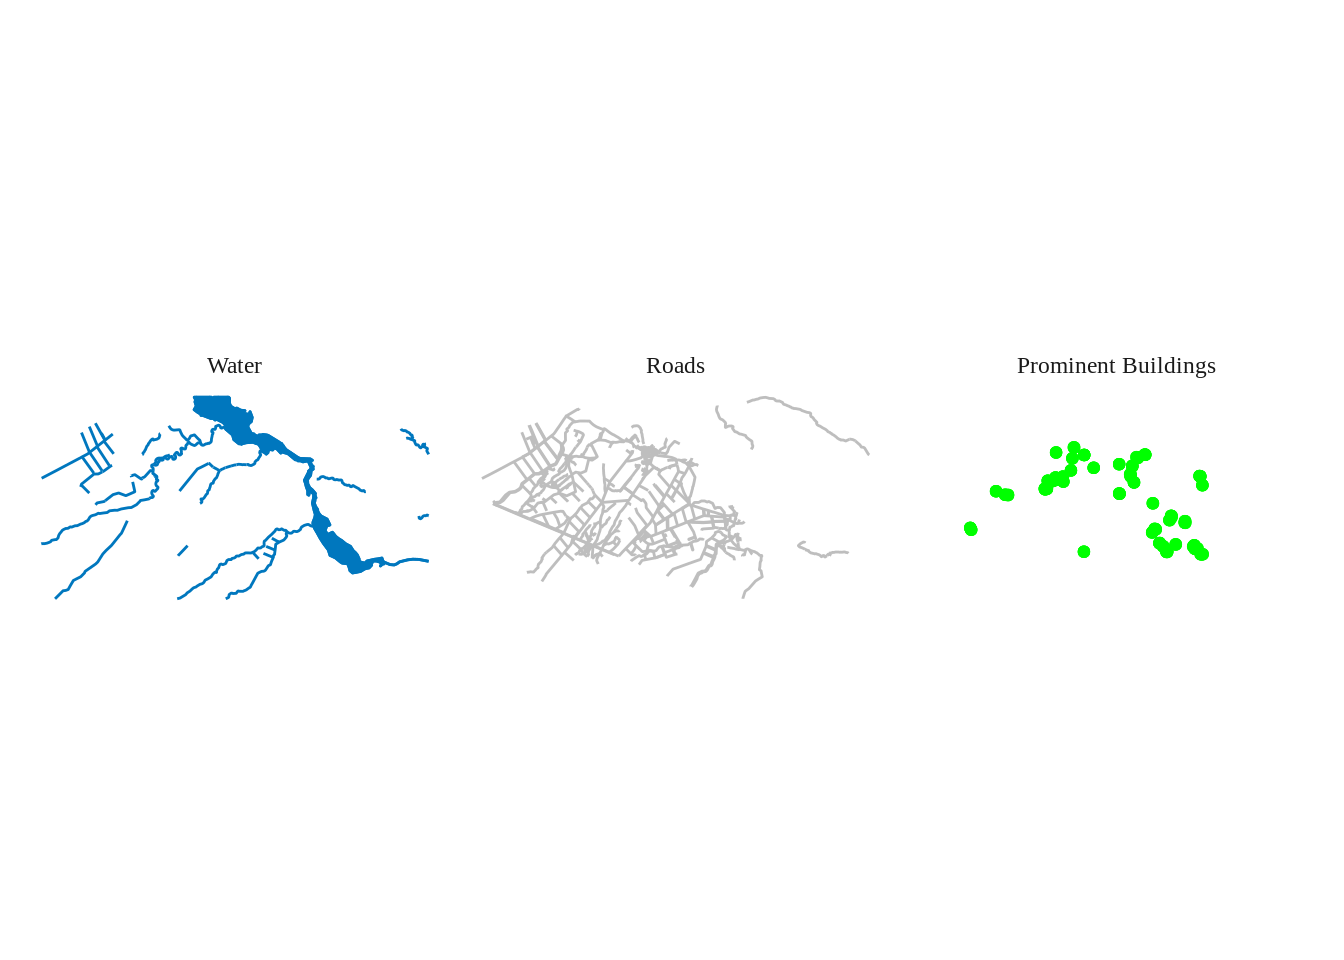
\includegraphics[width=1\linewidth]{3-spatial_files/figure-latex/unnamed-chunk-3-1} 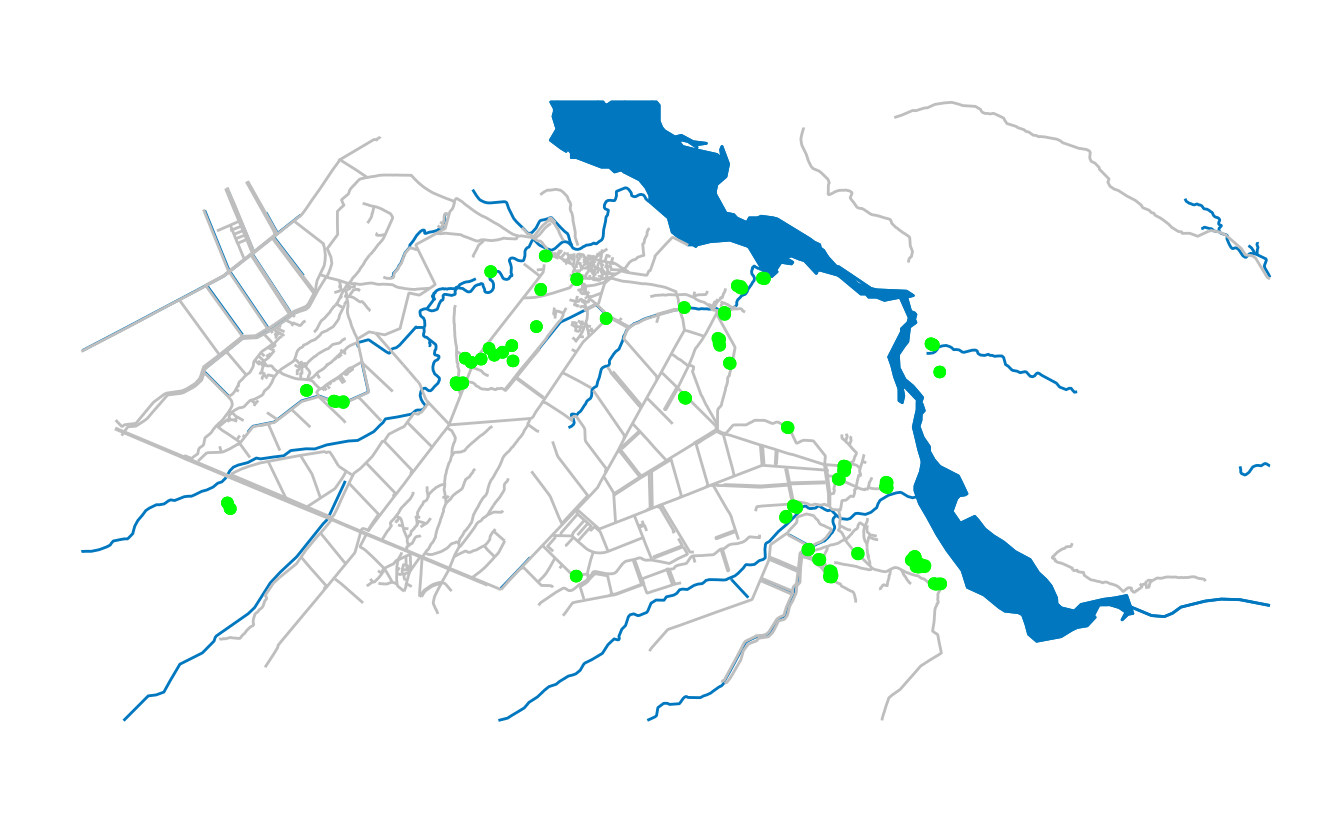
\includegraphics[width=1\linewidth]{3-spatial_files/figure-latex/unnamed-chunk-3-2} \end{center}

\begin{center}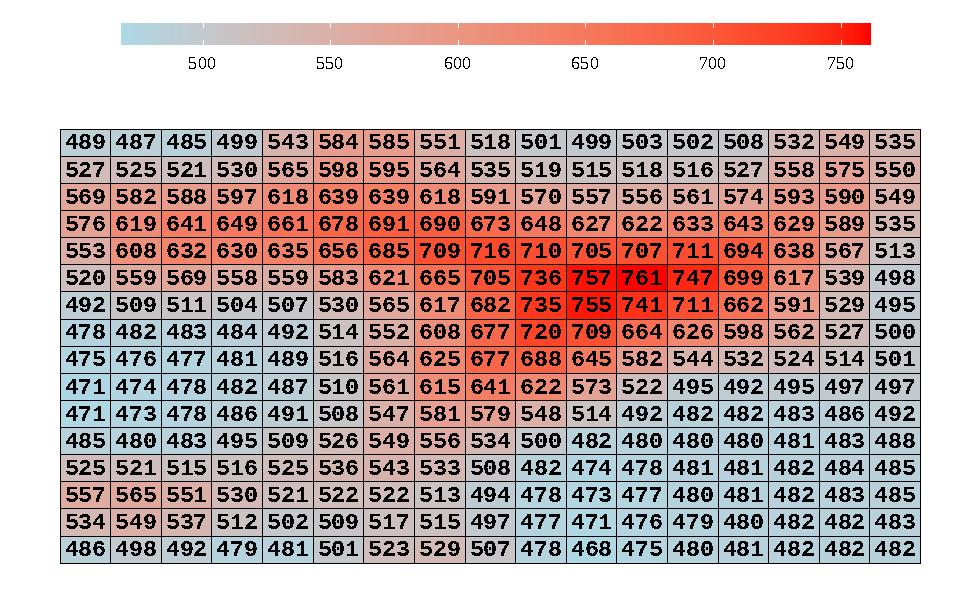
\includegraphics[width=1\linewidth]{3-spatial_files/figure-latex/unnamed-chunk-4-1} \end{center}

\begin{center}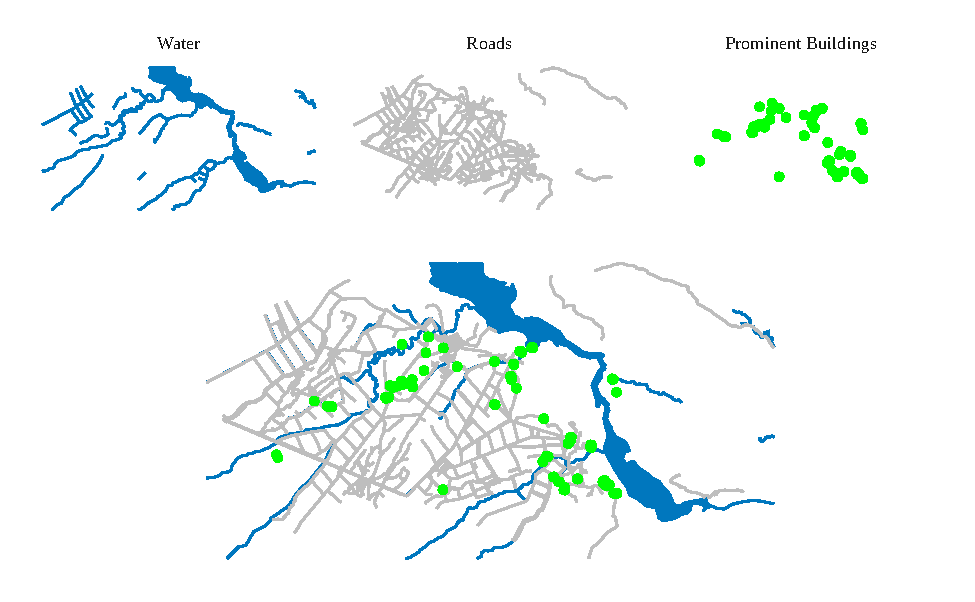
\includegraphics[width=1\linewidth]{3-spatial_files/figure-latex/unnamed-chunk-5-1} \end{center}

\begin{center}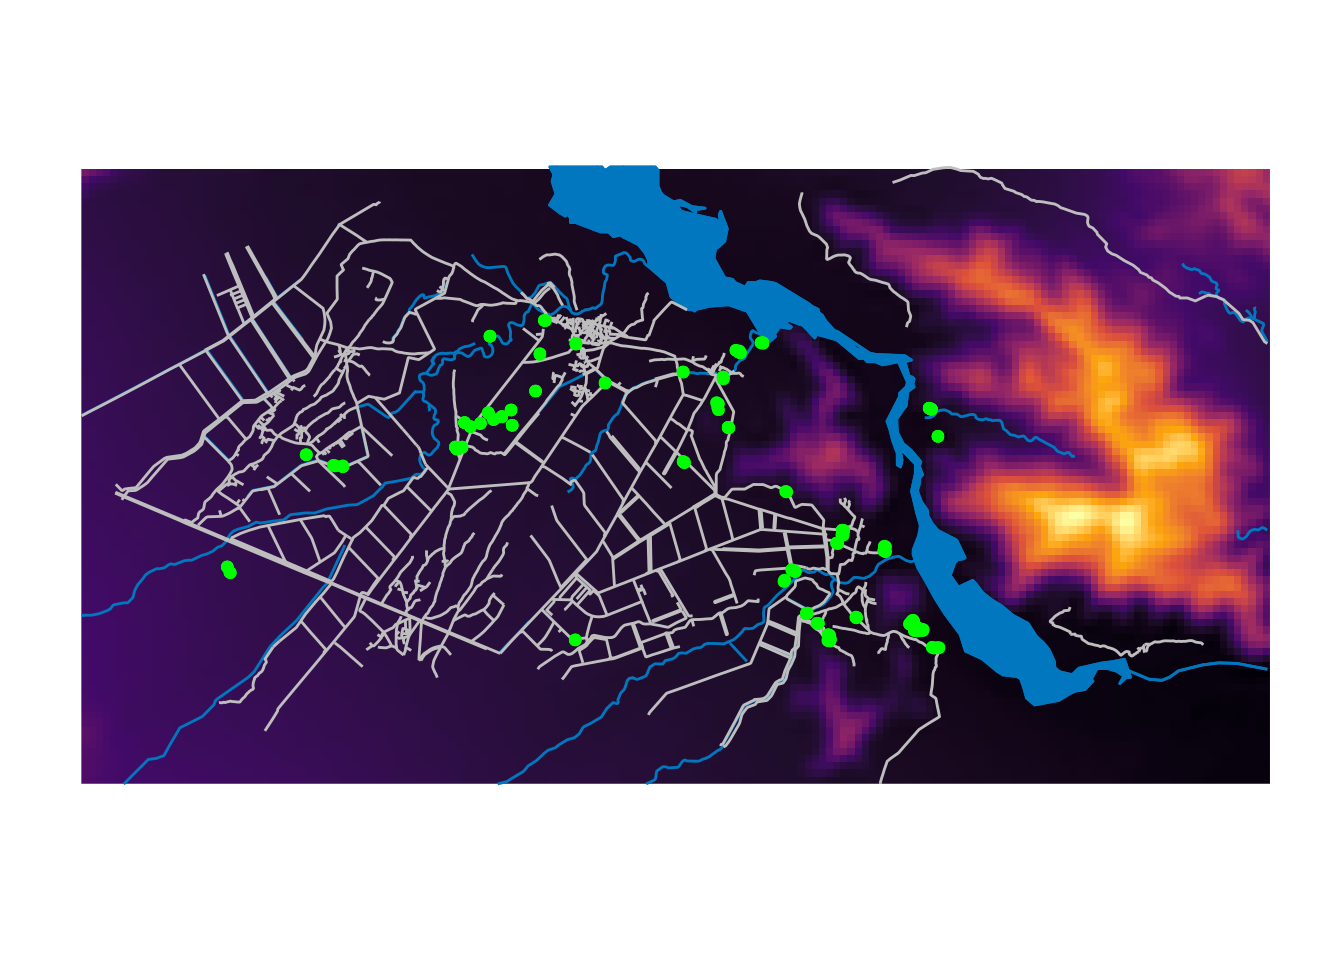
\includegraphics[width=1\linewidth]{3-spatial_files/figure-latex/unnamed-chunk-6-1} \end{center}

\hypertarget{geometry}{%
\section{\texorpdfstring{\texttt{geometry}}{geometry}}\label{geometry}}

Spatial vector data represent the world as a collection of points which, for two-dimensional data, are stored as \(x\) and \(y\) coordinates.

Points can be joined in order to make lines, which themselves can be joined to make polygons.

\begin{center}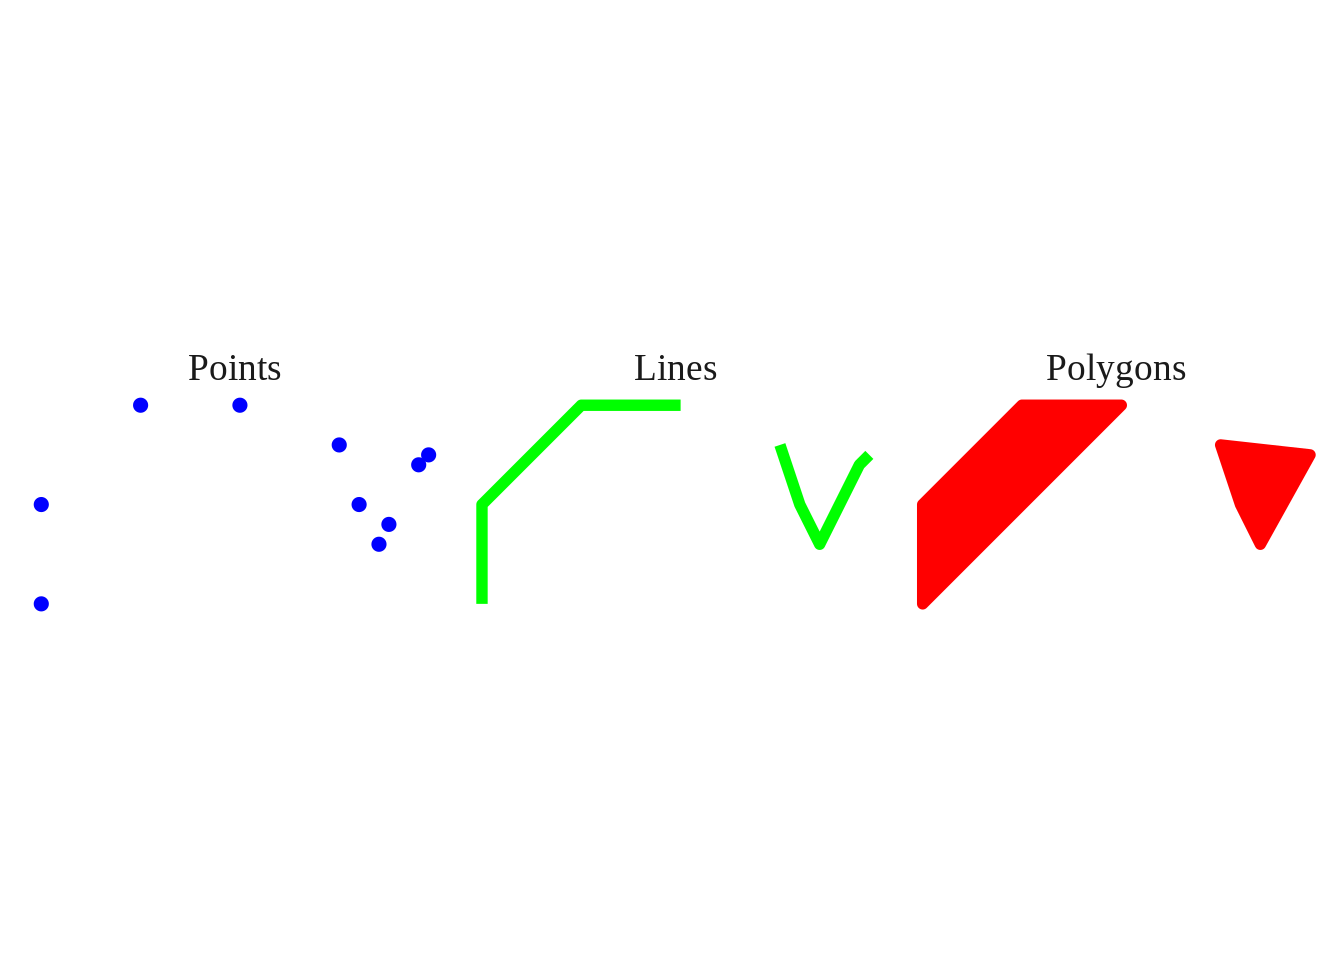
\includegraphics[width=1\linewidth]{3-spatial_files/figure-latex/unnamed-chunk-7-1} \end{center}

\begin{Shaded}
\begin{Highlighting}[]
\NormalTok{practice\_coords \textless{}{-}}\StringTok{ }\KeywordTok{tibble}\NormalTok{(}\DataTypeTok{lng =} \KeywordTok{c}\NormalTok{(}\OperatorTok{{-}}\DecValTok{20}\NormalTok{, }\DecValTok{{-}20}\NormalTok{, }\DecValTok{{-}10}\NormalTok{, }\DecValTok{{-}10}\NormalTok{, }\DecValTok{20}\NormalTok{, }\DecValTok{20}\NormalTok{,  }\DecValTok{10}\NormalTok{,  }\DecValTok{10}\NormalTok{), }
                          \DataTypeTok{lat =} \KeywordTok{c}\NormalTok{(}\OperatorTok{{-}}\DecValTok{20}\NormalTok{, }\DecValTok{10}\NormalTok{, }\DecValTok{20}\NormalTok{, }\DecValTok{{-}10}\NormalTok{, }\DecValTok{{-}10}\NormalTok{,  }\DecValTok{10}\NormalTok{,  }\DecValTok{20}\NormalTok{, }\DecValTok{{-}20}\NormalTok{),}
                          \DataTypeTok{lab =} \KeywordTok{c}\NormalTok{(}\StringTok{"A"}\NormalTok{, }\StringTok{"B"}\NormalTok{, }\StringTok{"C"}\NormalTok{, }\StringTok{"D"}\NormalTok{, }\StringTok{"E"}\NormalTok{, }\StringTok{"F"}\NormalTok{, }\StringTok{"G"}\NormalTok{, }\StringTok{"H"}\NormalTok{),}
                          \DataTypeTok{grp =} \KeywordTok{c}\NormalTok{(}\StringTok{"a"}\NormalTok{, }\StringTok{"a"}\NormalTok{, }\StringTok{"a"}\NormalTok{, }\StringTok{"a"}\NormalTok{, }\StringTok{"b"}\NormalTok{, }\StringTok{"b"}\NormalTok{, }\StringTok{"b"}\NormalTok{, }\StringTok{"b"}\NormalTok{))}
\NormalTok{practice\_coords}
\CommentTok{\#\textgreater{} \# A tibble: 8 x 4}
\CommentTok{\#\textgreater{}     lng   lat lab   grp  }
\CommentTok{\#\textgreater{}   \textless{}dbl\textgreater{} \textless{}dbl\textgreater{} \textless{}chr\textgreater{} \textless{}chr\textgreater{}}
\CommentTok{\#\textgreater{} 1   {-}20   {-}20 A     a    }
\CommentTok{\#\textgreater{} 2   {-}20    10 B     a    }
\CommentTok{\#\textgreater{} 3   {-}10    20 C     a    }
\CommentTok{\#\textgreater{} 4   {-}10   {-}10 D     a    }
\CommentTok{\#\textgreater{} 5    20   {-}10 E     b    }
\CommentTok{\#\textgreater{} 6    20    10 F     b    }
\CommentTok{\#\textgreater{} 7    10    20 G     b    }
\CommentTok{\#\textgreater{} 8    10   {-}20 H     b}
\end{Highlighting}
\end{Shaded}

\hypertarget{point}{%
\subsubsection{\texorpdfstring{\texttt{POINT}}{POINT}}\label{point}}

\texttt{POINT} refers to the location of a single point in space.

Here, we use \texttt{st\_as\_sf()} to convert a regular \texttt{data.frame} into an \texttt{sf} object.

\begin{itemize}
\tightlist
\item
  Steps:

  \begin{enumerate}
  \def\labelenumi{\arabic{enumi}.}
  \tightlist
  \item
    take \texttt{practice\_coords}
  \item
    convert to \texttt{sf} object with \texttt{st\_as\_sf()}, providing a \texttt{character} \texttt{vector} indicating the \texttt{names} of \texttt{practice\_coords} in \((x, y)\) / \((longitude, latitude)\) order
  \item
    \texttt{mutate()} to a add a column named \texttt{shape}, which we obtain using \texttt{st\_geometry\_type()}.
  \end{enumerate}
\end{itemize}

\begin{Shaded}
\begin{Highlighting}[]
\NormalTok{point\_sf \textless{}{-}}\StringTok{ }\NormalTok{practice\_coords }\OperatorTok{\%\textgreater{}\%}\StringTok{              }\CommentTok{\# Step 1.}
\StringTok{  }\KeywordTok{st\_as\_sf}\NormalTok{(}\DataTypeTok{coords =} \KeywordTok{c}\NormalTok{(}\StringTok{"lng"}\NormalTok{, }\StringTok{"lat"}\NormalTok{)) }\OperatorTok{\%\textgreater{}\%}\StringTok{     }\CommentTok{\# 2.}
\StringTok{  }\KeywordTok{mutate}\NormalTok{(}\DataTypeTok{shape =} \KeywordTok{st\_geometry\_type}\NormalTok{(geometry)) }\CommentTok{\# 3.}
\NormalTok{point\_sf}
\CommentTok{\#\textgreater{} Simple feature collection with 8 features and 3 fields}
\CommentTok{\#\textgreater{} geometry type:  POINT}
\CommentTok{\#\textgreater{} dimension:      XY}
\CommentTok{\#\textgreater{} bbox:           xmin: {-}20 ymin: {-}20 xmax: 20 ymax: 20}
\CommentTok{\#\textgreater{} CRS:            NA}
\CommentTok{\#\textgreater{} \# A tibble: 8 x 4}
\CommentTok{\#\textgreater{}   lab   grp    geometry shape}
\CommentTok{\#\textgreater{} * \textless{}chr\textgreater{} \textless{}chr\textgreater{}   \textless{}POINT\textgreater{} \textless{}fct\textgreater{}}
\CommentTok{\#\textgreater{} 1 A     a     ({-}20 {-}20) POINT}
\CommentTok{\#\textgreater{} 2 B     a      ({-}20 10) POINT}
\CommentTok{\#\textgreater{} 3 C     a      ({-}10 20) POINT}
\CommentTok{\#\textgreater{} 4 D     a     ({-}10 {-}10) POINT}
\CommentTok{\#\textgreater{} 5 E     b      (20 {-}10) POINT}
\CommentTok{\#\textgreater{} 6 F     b       (20 10) POINT}
\CommentTok{\#\textgreater{} 7 G     b       (10 20) POINT}
\CommentTok{\#\textgreater{} 8 H     b      (10 {-}20) POINT}
\end{Highlighting}
\end{Shaded}

The data in our \texttt{lng} and \texttt{lat} columns are moved to a new \texttt{geometry} column.

\begin{Shaded}
\begin{Highlighting}[]
\KeywordTok{ggplot}\NormalTok{(}\DataTypeTok{data =}\NormalTok{ point\_sf) }\OperatorTok{+}\StringTok{ }
\StringTok{  }\KeywordTok{geom\_sf}\NormalTok{(}\KeywordTok{aes}\NormalTok{(}\DataTypeTok{color =}\NormalTok{ lab), }\DataTypeTok{size =} \DecValTok{5}\NormalTok{, }\DataTypeTok{show.legend =} \StringTok{"point"}\NormalTok{) }\OperatorTok{+}
\StringTok{  }\KeywordTok{labs}\NormalTok{(}\DataTypeTok{title =} \StringTok{"POINT"}\NormalTok{)}
\end{Highlighting}
\end{Shaded}

\begin{center}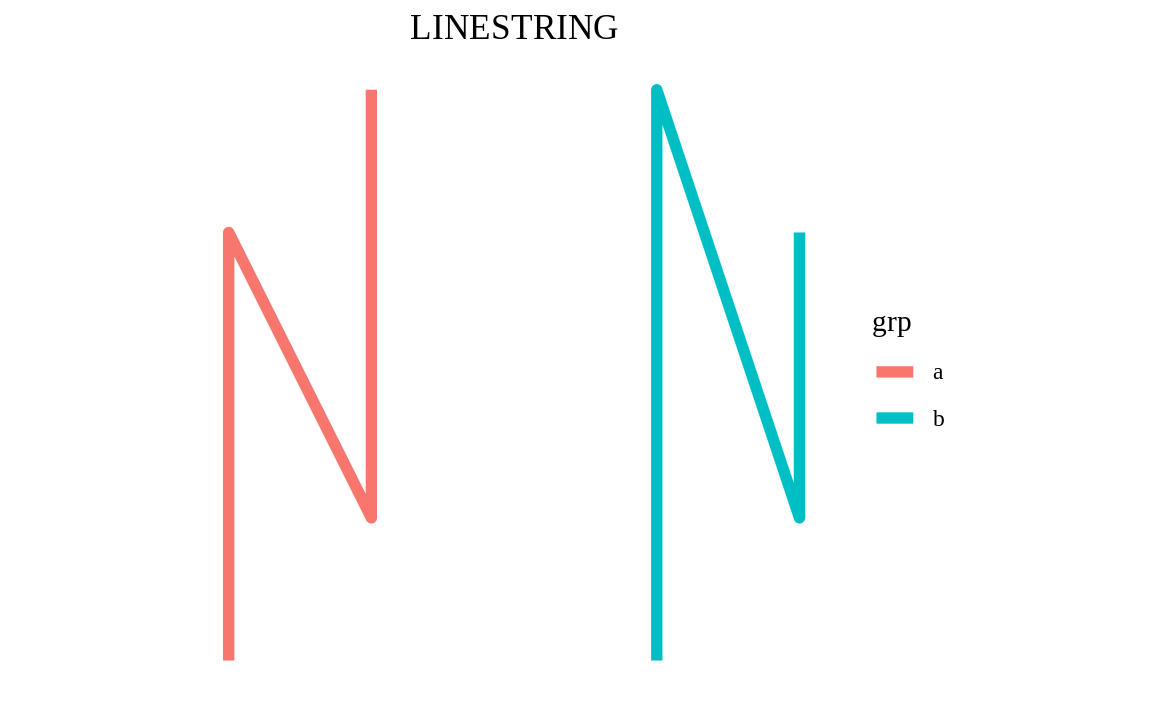
\includegraphics[width=1\linewidth]{3-spatial_files/figure-latex/unnamed-chunk-10-1} \end{center}

\hypertarget{multipoint}{%
\subsubsection{\texorpdfstring{\texttt{MULTIPOINT}}{MULTIPOINT}}\label{multipoint}}

\texttt{MULTIPOINT} refers to a collection of \texttt{POINT}s.

\begin{itemize}
\tightlist
\item
  Steps:

  \begin{enumerate}
  \def\labelenumi{\arabic{enumi}.}
  \tightlist
  \item
    take \texttt{point\_sf}
  \item
    using \texttt{group\_by()}, group the rows together based on the values in their \texttt{grp} column
  \item
    \texttt{summarise()} each group, which combines the points of each group into a \texttt{MULTIPOINT}
  \item
    \texttt{mutate()} the \texttt{shape} column to change it to the new \texttt{st\_geometry\_type()}
  \end{enumerate}
\end{itemize}

\begin{Shaded}
\begin{Highlighting}[]
\NormalTok{multi\_point\_sf \textless{}{-}}\StringTok{ }\NormalTok{point\_sf }\OperatorTok{\%\textgreater{}\%}\StringTok{               }\CommentTok{\# Step 1.}
\StringTok{  }\KeywordTok{group\_by}\NormalTok{(grp) }\OperatorTok{\%\textgreater{}\%}\StringTok{                          }\CommentTok{\# 2.}
\StringTok{  }\KeywordTok{summarise}\NormalTok{() }\OperatorTok{\%\textgreater{}\%}\StringTok{                            }\CommentTok{\# 3.}
\StringTok{  }\KeywordTok{mutate}\NormalTok{(}\DataTypeTok{shape =} \KeywordTok{st\_geometry\_type}\NormalTok{(geometry)) }\CommentTok{\# 4.}
\CommentTok{\#\textgreater{} \textasciigrave{}summarise()\textasciigrave{} ungrouping output (override with \textasciigrave{}.groups\textasciigrave{} argument)}

\NormalTok{multi\_point\_sf}
\CommentTok{\#\textgreater{} Simple feature collection with 2 features and 2 fields}
\CommentTok{\#\textgreater{} geometry type:  MULTIPOINT}
\CommentTok{\#\textgreater{} dimension:      XY}
\CommentTok{\#\textgreater{} bbox:           xmin: {-}20 ymin: {-}20 xmax: 20 ymax: 20}
\CommentTok{\#\textgreater{} CRS:            NA}
\CommentTok{\#\textgreater{} \# A tibble: 2 x 3}
\CommentTok{\#\textgreater{}   grp                                     geometry shape     }
\CommentTok{\#\textgreater{} * \textless{}chr\textgreater{}                               \textless{}MULTIPOINT\textgreater{} \textless{}fct\textgreater{}     }
\CommentTok{\#\textgreater{} 1 a     (({-}20 {-}20), ({-}20 10), ({-}10 {-}10), ({-}10 20)) MULTIPOINT}
\CommentTok{\#\textgreater{} 2 b         ((10 {-}20), (10 20), (20 {-}10), (20 10)) MULTIPOINT}
\end{Highlighting}
\end{Shaded}

Instead of the 8 separate \texttt{POINT}s with which we started, we now have 2 rows of \texttt{MULTIPOINT}s, each of which contain 4 points.

\begin{Shaded}
\begin{Highlighting}[]
\KeywordTok{ggplot}\NormalTok{(}\DataTypeTok{data =}\NormalTok{ multi\_point\_sf) }\OperatorTok{+}\StringTok{ }
\StringTok{  }\KeywordTok{geom\_sf}\NormalTok{(}\KeywordTok{aes}\NormalTok{(}\DataTypeTok{color =}\NormalTok{ grp), }\DataTypeTok{size =} \DecValTok{5}\NormalTok{, }\DataTypeTok{show.legend =} \StringTok{"point"}\NormalTok{) }\OperatorTok{+}
\StringTok{  }\KeywordTok{labs}\NormalTok{(}\DataTypeTok{title =} \StringTok{"MULTIPOINT"}\NormalTok{)}
\end{Highlighting}
\end{Shaded}

\begin{center}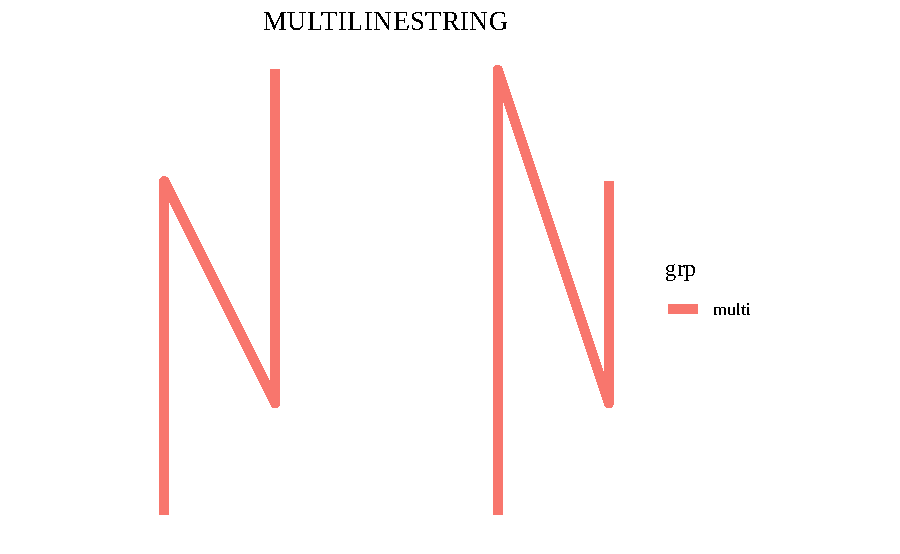
\includegraphics[width=1\linewidth]{3-spatial_files/figure-latex/unnamed-chunk-12-1} \end{center}

\hypertarget{linestring}{%
\subsubsection{\texorpdfstring{\texttt{LINESTRING}}{LINESTRING}}\label{linestring}}

\texttt{LINESTRING} is how we represent individual lines.

\begin{itemize}
\tightlist
\item
  Steps:

  \begin{enumerate}
  \def\labelenumi{\arabic{enumi}.}
  \tightlist
  \item
    take \texttt{multi\_point\_sf}
  \item
    cast the \texttt{geometry} \texttt{to=} \texttt{LINESTRING} using \texttt{st\_cast()}
    3 \texttt{mutate()} the \texttt{shape} column to change it to the new \texttt{st\_geometry\_type()}
  \end{enumerate}
\end{itemize}

\begin{Shaded}
\begin{Highlighting}[]
\NormalTok{linestring\_sf \textless{}{-}}\StringTok{ }\NormalTok{multi\_point\_sf }\OperatorTok{\%\textgreater{}\%}\StringTok{          }\CommentTok{\# Step 1.}
\StringTok{  }\KeywordTok{st\_cast}\NormalTok{(}\DataTypeTok{to =} \StringTok{"LINESTRING"}\NormalTok{) }\OperatorTok{\%\textgreater{}\%}\StringTok{             }\CommentTok{\# 2.}
\StringTok{  }\KeywordTok{mutate}\NormalTok{(}\DataTypeTok{shape =} \KeywordTok{st\_geometry\_type}\NormalTok{(geometry)) }\CommentTok{\# 3.}

\NormalTok{linestring\_sf}
\CommentTok{\#\textgreater{} Simple feature collection with 2 features and 2 fields}
\CommentTok{\#\textgreater{} geometry type:  LINESTRING}
\CommentTok{\#\textgreater{} dimension:      XY}
\CommentTok{\#\textgreater{} bbox:           xmin: {-}20 ymin: {-}20 xmax: 20 ymax: 20}
\CommentTok{\#\textgreater{} CRS:            NA}
\CommentTok{\#\textgreater{} \# A tibble: 2 x 3}
\CommentTok{\#\textgreater{}   grp   shape                                geometry}
\CommentTok{\#\textgreater{} * \textless{}chr\textgreater{} \textless{}fct\textgreater{}                            \textless{}LINESTRING\textgreater{}}
\CommentTok{\#\textgreater{} 1 a     LINESTRING ({-}20 {-}20, {-}20 10, {-}10 {-}10, {-}10 20)}
\CommentTok{\#\textgreater{} 2 b     LINESTRING     (10 {-}20, 10 20, 20 {-}10, 20 10)}
\end{Highlighting}
\end{Shaded}

Now we have 2 rows that each contain a \texttt{LINESTRING}, which was built by connecting each point to the next.

\begin{Shaded}
\begin{Highlighting}[]
\KeywordTok{ggplot}\NormalTok{(}\DataTypeTok{data =}\NormalTok{ linestring\_sf) }\OperatorTok{+}\StringTok{ }
\StringTok{  }\KeywordTok{geom\_sf}\NormalTok{(}\KeywordTok{aes}\NormalTok{(}\DataTypeTok{color =}\NormalTok{ grp), }\DataTypeTok{size =} \DecValTok{2}\NormalTok{, }\DataTypeTok{show.legend =} \StringTok{"line"}\NormalTok{) }\OperatorTok{+}
\StringTok{  }\KeywordTok{labs}\NormalTok{(}\DataTypeTok{title =} \StringTok{"LINESTRING"}\NormalTok{)}
\end{Highlighting}
\end{Shaded}

\begin{center}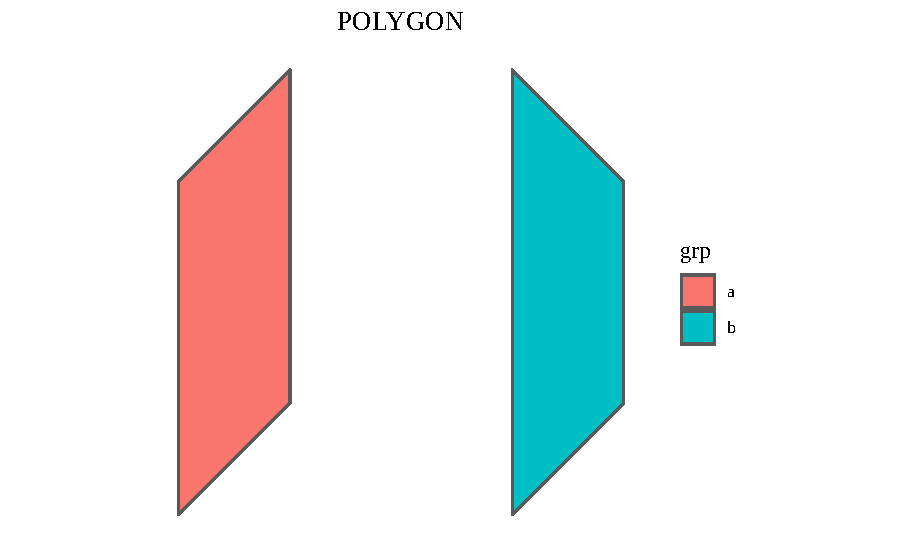
\includegraphics[width=1\linewidth]{3-spatial_files/figure-latex/unnamed-chunk-14-1} \end{center}

\hypertarget{multilinestring}{%
\subsubsection{\texorpdfstring{\texttt{MULTILINESTRING}}{MULTILINESTRING}}\label{multilinestring}}

Similar to \texttt{MULTIPOINT}s that contain multiple points, we also have \texttt{MULTILINESTRING}s.

\begin{itemize}
\tightlist
\item
  Steps:

  \begin{enumerate}
  \def\labelenumi{\arabic{enumi}.}
  \tightlist
  \item
    take \texttt{linestring\_sf}
  \item
    \texttt{summarise()} the rows, combining them all into a single \texttt{MULTILINESTRING}
  \item
    \texttt{mutate()} the \texttt{shape} column to change it to the new \texttt{st\_geometry\_type()} and replace the \texttt{grp} column that is dropped when we \texttt{summarise()} without using \texttt{group\_by()}
  \end{enumerate}
\end{itemize}

\begin{Shaded}
\begin{Highlighting}[]
\NormalTok{multi\_linestring\_sf \textless{}{-}}\StringTok{ }\NormalTok{linestring\_sf }\OperatorTok{\%\textgreater{}\%}\StringTok{     }\CommentTok{\# Step 1.}
\StringTok{  }\KeywordTok{summarise}\NormalTok{() }\OperatorTok{\%\textgreater{}\%}\StringTok{                            }\CommentTok{\# 2.}
\StringTok{  }\KeywordTok{mutate}\NormalTok{(}\DataTypeTok{shape =} \KeywordTok{st\_geometry\_type}\NormalTok{(geometry), }\CommentTok{\# 3.}
         \DataTypeTok{grp =} \StringTok{"multi"}\NormalTok{)                      }\CommentTok{\# 4.}

\NormalTok{multi\_linestring\_sf}
\CommentTok{\#\textgreater{} Simple feature collection with 1 feature and 2 fields}
\CommentTok{\#\textgreater{} geometry type:  MULTILINESTRING}
\CommentTok{\#\textgreater{} dimension:      XY}
\CommentTok{\#\textgreater{} bbox:           xmin: {-}20 ymin: {-}20 xmax: 20 ymax: 20}
\CommentTok{\#\textgreater{} CRS:            NA}
\CommentTok{\#\textgreater{} \# A tibble: 1 x 3}
\CommentTok{\#\textgreater{}                                                               geometry shape           grp  }
\CommentTok{\#\textgreater{} *                                                    \textless{}MULTILINESTRING\textgreater{} \textless{}fct\textgreater{}           \textless{}chr\textgreater{}}
\CommentTok{\#\textgreater{} 1 (({-}20 {-}20, {-}20 10, {-}10 {-}10, {-}10 20), (10 {-}20, 10 20, 20 {-}10, 20 10)) MULTILINESTRING multi}
\end{Highlighting}
\end{Shaded}

Now we have 2 lines embedded inside a single \texttt{MULTILINESTRING} row.

\begin{Shaded}
\begin{Highlighting}[]
\KeywordTok{ggplot}\NormalTok{(}\DataTypeTok{data =}\NormalTok{ multi\_linestring\_sf) }\OperatorTok{+}\StringTok{ }
\StringTok{  }\KeywordTok{geom\_sf}\NormalTok{(}\KeywordTok{aes}\NormalTok{(}\DataTypeTok{color =}\NormalTok{ grp), }\DataTypeTok{size =} \DecValTok{2}\NormalTok{, }\DataTypeTok{show.legend =} \StringTok{"line"}\NormalTok{) }\OperatorTok{+}
\StringTok{  }\KeywordTok{labs}\NormalTok{(}\DataTypeTok{title =} \StringTok{"MULTILINESTRING"}\NormalTok{)}
\end{Highlighting}
\end{Shaded}

\begin{center}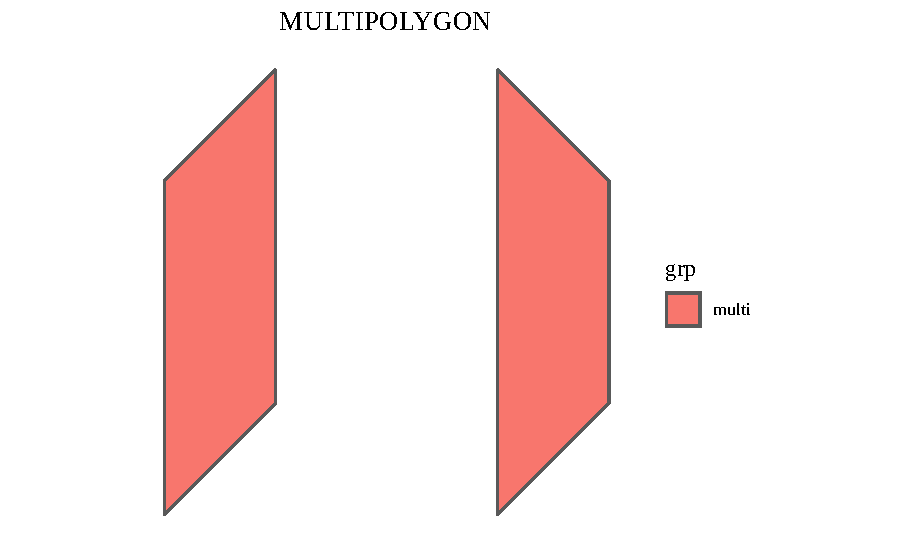
\includegraphics[width=1\linewidth]{3-spatial_files/figure-latex/unnamed-chunk-16-1} \end{center}

\hypertarget{polygon}{%
\subsubsection{\texorpdfstring{\texttt{POLYGON}}{POLYGON}}\label{polygon}}

\texttt{POLYGON}s are essentially sets of lines that close to form a ring, although \texttt{POLGYON}s can also contain holes. We can easily wrap a shape around any \texttt{geometry} using \texttt{st\_convex\_hull()} to form a \href{https://en.wikipedia.org/wiki/Convex_hull}{convex hull} polygon.

\begin{itemize}
\tightlist
\item
  Steps:

  \begin{enumerate}
  \def\labelenumi{\arabic{enumi}.}
  \tightlist
  \item
    take \texttt{point\_sf}
  \item
    using \texttt{group\_by()}, group the rows together based on the values in their \texttt{grp} column
  \item
    \texttt{summarise()} each group, combining them into \texttt{MULTIPOINT}s
  \item
    wrap the \texttt{MULTIPOINT}s in a polygon using \texttt{st\_convex\_hull()}
  \item
    \texttt{mutate()} the \texttt{shape} column to change it to the new \texttt{st\_geometry\_type()}
  \end{enumerate}
\end{itemize}

\begin{Shaded}
\begin{Highlighting}[]
\NormalTok{polygon\_sf \textless{}{-}}\StringTok{ }\NormalTok{point\_sf }\OperatorTok{\%\textgreater{}\%}\StringTok{                   }\CommentTok{\# Step 1.}
\StringTok{  }\KeywordTok{group\_by}\NormalTok{(grp) }\OperatorTok{\%\textgreater{}\%}\StringTok{                          }\CommentTok{\# 2.}
\StringTok{  }\KeywordTok{summarise}\NormalTok{() }\OperatorTok{\%\textgreater{}\%}\StringTok{                            }\CommentTok{\# 3.}
\StringTok{  }\KeywordTok{st\_convex\_hull}\NormalTok{() }\OperatorTok{\%\textgreater{}\%}\StringTok{                       }\CommentTok{\# 4.}
\StringTok{  }\KeywordTok{mutate}\NormalTok{(}\DataTypeTok{shape =} \KeywordTok{st\_geometry\_type}\NormalTok{(geometry)) }\CommentTok{\# 5.}
\CommentTok{\#\textgreater{} \textasciigrave{}summarise()\textasciigrave{} ungrouping output (override with \textasciigrave{}.groups\textasciigrave{} argument)}

\NormalTok{polygon\_sf}
\CommentTok{\#\textgreater{} Simple feature collection with 2 features and 2 fields}
\CommentTok{\#\textgreater{} geometry type:  POLYGON}
\CommentTok{\#\textgreater{} dimension:      XY}
\CommentTok{\#\textgreater{} bbox:           xmin: {-}20 ymin: {-}20 xmax: 20 ymax: 20}
\CommentTok{\#\textgreater{} CRS:            NA}
\CommentTok{\#\textgreater{} \# A tibble: 2 x 3}
\CommentTok{\#\textgreater{}   grp                                        geometry shape  }
\CommentTok{\#\textgreater{} * \textless{}chr\textgreater{}                                     \textless{}POLYGON\textgreater{} \textless{}fct\textgreater{}  }
\CommentTok{\#\textgreater{} 1 a     (({-}20 {-}20, {-}20 10, {-}10 20, {-}10 {-}10, {-}20 {-}20)) POLYGON}
\CommentTok{\#\textgreater{} 2 b          ((10 {-}20, 10 20, 20 10, 20 {-}10, 10 {-}20)) POLYGON}
\end{Highlighting}
\end{Shaded}

\begin{Shaded}
\begin{Highlighting}[]
\KeywordTok{ggplot}\NormalTok{(}\DataTypeTok{data =}\NormalTok{ polygon\_sf) }\OperatorTok{+}\StringTok{ }
\StringTok{  }\KeywordTok{geom\_sf}\NormalTok{(}\KeywordTok{aes}\NormalTok{(}\DataTypeTok{fill =}\NormalTok{ grp), }\DataTypeTok{show.legend =} \StringTok{"polygon"}\NormalTok{) }\OperatorTok{+}
\StringTok{  }\KeywordTok{labs}\NormalTok{(}\DataTypeTok{title =} \StringTok{"POLYGON"}\NormalTok{)}
\end{Highlighting}
\end{Shaded}

\begin{center}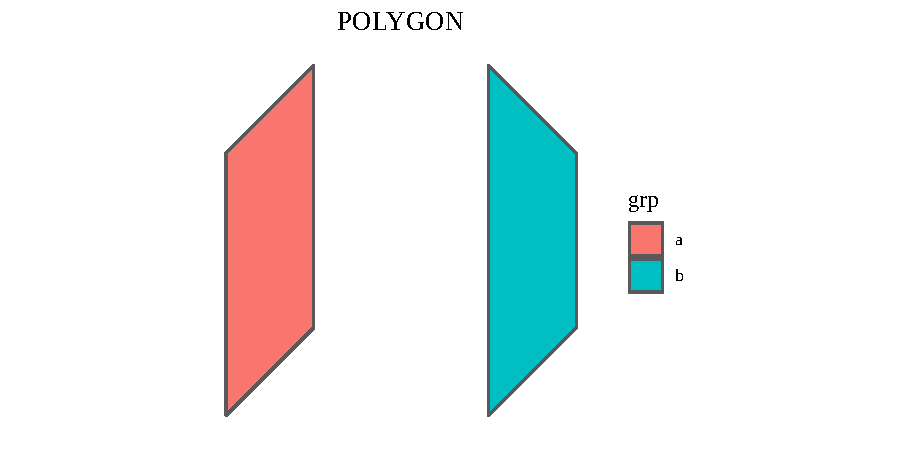
\includegraphics[width=1\linewidth]{3-spatial_files/figure-latex/unnamed-chunk-18-1} \end{center}

\hypertarget{multipolygon}{%
\subsubsection{\texorpdfstring{\texttt{MULTIPOLYGON}}{MULTIPOLYGON}}\label{multipolygon}}

\texttt{POLYGON}s can also be grouped together to form \texttt{MULTIPOLYGON}s.

\begin{itemize}
\tightlist
\item
  Steps:

  \begin{enumerate}
  \def\labelenumi{\arabic{enumi}.}
  \tightlist
  \item
    take \texttt{polygon\_sf}
  \item
    \texttt{summarise()} the rows, combining them all into a single \texttt{MULTILIPOLYGON}
  \item
    \texttt{mutate()} the \texttt{shape} column to change it to the new \texttt{st\_geometry\_type()} and replace the \texttt{grp} column that is dropped when we \texttt{summarise()} without using \texttt{group\_by()}
  \end{enumerate}
\end{itemize}

\begin{Shaded}
\begin{Highlighting}[]
\NormalTok{multi\_polygon\_sf \textless{}{-}}\StringTok{ }\NormalTok{polygon\_sf }\OperatorTok{\%\textgreater{}\%}\StringTok{           }\CommentTok{\# Step 1.}
\StringTok{  }\KeywordTok{summarise}\NormalTok{() }\OperatorTok{\%\textgreater{}\%}\StringTok{                            }\CommentTok{\# 2.}
\StringTok{  }\KeywordTok{mutate}\NormalTok{(}\DataTypeTok{shape =} \KeywordTok{st\_geometry\_type}\NormalTok{(geometry), }\CommentTok{\# 3.}
         \DataTypeTok{grp =} \StringTok{"multi"}\NormalTok{)}

\NormalTok{multi\_polygon\_sf}
\CommentTok{\#\textgreater{} Simple feature collection with 1 feature and 2 fields}
\CommentTok{\#\textgreater{} geometry type:  MULTIPOLYGON}
\CommentTok{\#\textgreater{} dimension:      XY}
\CommentTok{\#\textgreater{} bbox:           xmin: {-}20 ymin: {-}20 xmax: 20 ymax: 20}
\CommentTok{\#\textgreater{} CRS:            NA}
\CommentTok{\#\textgreater{} \# A tibble: 1 x 3}
\CommentTok{\#\textgreater{}                                                                       geometry shape      grp  }
\CommentTok{\#\textgreater{} *                                                               \textless{}MULTIPOLYGON\textgreater{} \textless{}fct\textgreater{}      \textless{}chr\textgreater{}}
\CommentTok{\#\textgreater{} 1 ((({-}20 {-}20, {-}20 10, {-}10 20, {-}10 {-}10, {-}20 {-}20)), ((10 {-}20, 10 20, 20 10, 20 \textasciitilde{} MULTIPOLY\textasciitilde{} multi}
\end{Highlighting}
\end{Shaded}

\begin{Shaded}
\begin{Highlighting}[]
\KeywordTok{ggplot}\NormalTok{(}\DataTypeTok{data =}\NormalTok{ multi\_polygon\_sf) }\OperatorTok{+}
\StringTok{  }\KeywordTok{geom\_sf}\NormalTok{(}\KeywordTok{aes}\NormalTok{(}\DataTypeTok{fill =}\NormalTok{ grp), }\DataTypeTok{show.legend =} \StringTok{"polygon"}\NormalTok{) }\OperatorTok{+}
\StringTok{  }\KeywordTok{labs}\NormalTok{(}\DataTypeTok{title =} \StringTok{"MULTIPOLYGON"}\NormalTok{)}
\end{Highlighting}
\end{Shaded}

\begin{center}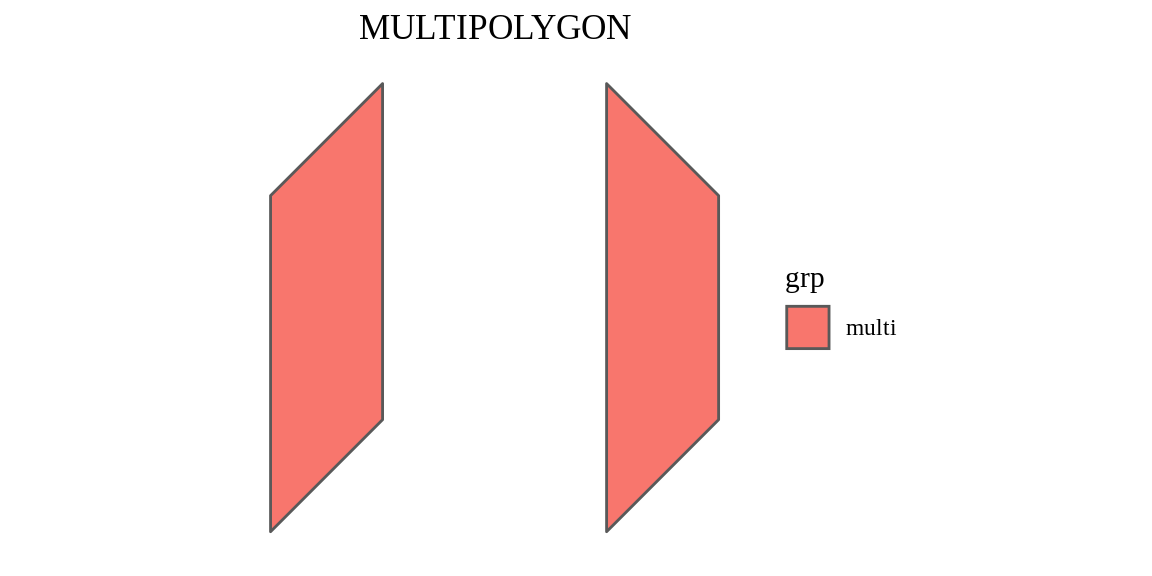
\includegraphics[width=1\linewidth]{3-spatial_files/figure-latex/unnamed-chunk-20-1} \end{center}

\hypertarget{geometry-1}{%
\subsubsection{\texorpdfstring{\texttt{GEOMETRY}}{GEOMETRY}}\label{geometry-1}}

\texttt{GEOMETRY} is a special \texttt{geometry} type. It refers to a column of mixed geometries, i.e.~we have multiple geometry types in our \texttt{geometry} column.

\begin{Shaded}
\begin{Highlighting}[]
\NormalTok{geometry\_sf \textless{}{-}}\StringTok{ }\KeywordTok{list}\NormalTok{(point\_sf, multi\_point\_sf, linestring\_sf, }
\NormalTok{                    multi\_linestring\_sf, polygon\_sf, multi\_polygon\_sf) }\OperatorTok{\%\textgreater{}\%}\StringTok{ }
\StringTok{  }\KeywordTok{map\_if}\NormalTok{(}\OperatorTok{\textasciitilde{}}\StringTok{ "lab"} \OperatorTok{\%in\%}\StringTok{ }\KeywordTok{names}\NormalTok{(.x), select, }\OperatorTok{{-}}\NormalTok{lab) }\OperatorTok{\%\textgreater{}\%}
\StringTok{  }\KeywordTok{do.call}\NormalTok{(}\DataTypeTok{what =}\NormalTok{ rbind) }\OperatorTok{\%\textgreater{}\%}\StringTok{ }
\StringTok{  }\KeywordTok{mutate}\NormalTok{(}\DataTypeTok{grp =} \KeywordTok{if\_else}\NormalTok{(shape }\OperatorTok{==}\StringTok{ "POINT"}\NormalTok{, }\KeywordTok{as.character}\NormalTok{(}\KeywordTok{row\_number}\NormalTok{()), grp))}

\NormalTok{geometry\_sf}
\CommentTok{\#\textgreater{} Simple feature collection with 16 features and 2 fields}
\CommentTok{\#\textgreater{} geometry type:  GEOMETRY}
\CommentTok{\#\textgreater{} dimension:      XY}
\CommentTok{\#\textgreater{} bbox:           xmin: {-}20 ymin: {-}20 xmax: 20 ymax: 20}
\CommentTok{\#\textgreater{} CRS:            NA}
\CommentTok{\#\textgreater{} \# A tibble: 16 x 3}
\CommentTok{\#\textgreater{}    grp                                                                    geometry shape       }
\CommentTok{\#\textgreater{}  * \textless{}chr\textgreater{}                                                                \textless{}GEOMETRY\textgreater{} \textless{}fct\textgreater{}       }
\CommentTok{\#\textgreater{}  1 1                                                               POINT ({-}20 {-}20) POINT       }
\CommentTok{\#\textgreater{}  2 2                                                                POINT ({-}20 10) POINT       }
\CommentTok{\#\textgreater{}  3 3                                                                POINT ({-}10 20) POINT       }
\CommentTok{\#\textgreater{}  4 4                                                               POINT ({-}10 {-}10) POINT       }
\CommentTok{\#\textgreater{}  5 5                                                                POINT (20 {-}10) POINT       }
\CommentTok{\#\textgreater{}  6 6                                                                 POINT (20 10) POINT       }
\CommentTok{\#\textgreater{}  7 7                                                                 POINT (10 20) POINT       }
\CommentTok{\#\textgreater{}  8 8                                                                POINT (10 {-}20) POINT       }
\CommentTok{\#\textgreater{}  9 a                         MULTIPOINT (({-}20 {-}20), ({-}20 10), ({-}10 {-}10), ({-}10 20)) MULTIPOINT  }
\CommentTok{\#\textgreater{} 10 b                             MULTIPOINT ((10 {-}20), (10 20), (20 {-}10), (20 10)) MULTIPOINT  }
\CommentTok{\#\textgreater{} 11 a                                 LINESTRING ({-}20 {-}20, {-}20 10, {-}10 {-}10, {-}10 20) LINESTRING  }
\CommentTok{\#\textgreater{} 12 b                                     LINESTRING (10 {-}20, 10 20, 20 {-}10, 20 10) LINESTRING  }
\CommentTok{\#\textgreater{} 13 multi MULTILINESTRING (({-}20 {-}20, {-}20 10, {-}10 {-}10, {-}10 20), (10 {-}20, 10 20, 20 \textasciitilde{} MULTILINEST\textasciitilde{}}
\CommentTok{\#\textgreater{} 14 a                         POLYGON (({-}20 {-}20, {-}20 10, {-}10 20, {-}10 {-}10, {-}20 {-}20)) POLYGON     }
\CommentTok{\#\textgreater{} 15 b                              POLYGON ((10 {-}20, 10 20, 20 10, 20 {-}10, 10 {-}20)) POLYGON     }
\CommentTok{\#\textgreater{} 16 multi MULTIPOLYGON ((({-}20 {-}20, {-}20 10, {-}10 20, {-}10 {-}10, {-}20 {-}20)), ((10 {-}20, 1\textasciitilde{} MULTIPOLYGON}
\end{Highlighting}
\end{Shaded}

\begin{Shaded}
\begin{Highlighting}[]
\KeywordTok{ggplot}\NormalTok{(}\DataTypeTok{data =}\NormalTok{ geometry\_sf) }\OperatorTok{+}
\StringTok{  }\KeywordTok{geom\_sf}\NormalTok{(}\KeywordTok{aes}\NormalTok{(}\DataTypeTok{color =}\NormalTok{ grp, }\DataTypeTok{fill =}\NormalTok{ grp), }\DataTypeTok{size =} \DecValTok{2}\NormalTok{, }\DataTypeTok{show.legend =} \OtherTok{FALSE}\NormalTok{) }\OperatorTok{+}
\StringTok{  }\KeywordTok{facet\_wrap}\NormalTok{(}\OperatorTok{\textasciitilde{}}\StringTok{ }\NormalTok{shape, }\DataTypeTok{nrow =} \DecValTok{2}\NormalTok{) }\OperatorTok{+}
\StringTok{  }\KeywordTok{labs}\NormalTok{(}\DataTypeTok{title =} \StringTok{"GEOMETRY"}\NormalTok{)}
\end{Highlighting}
\end{Shaded}

\begin{center}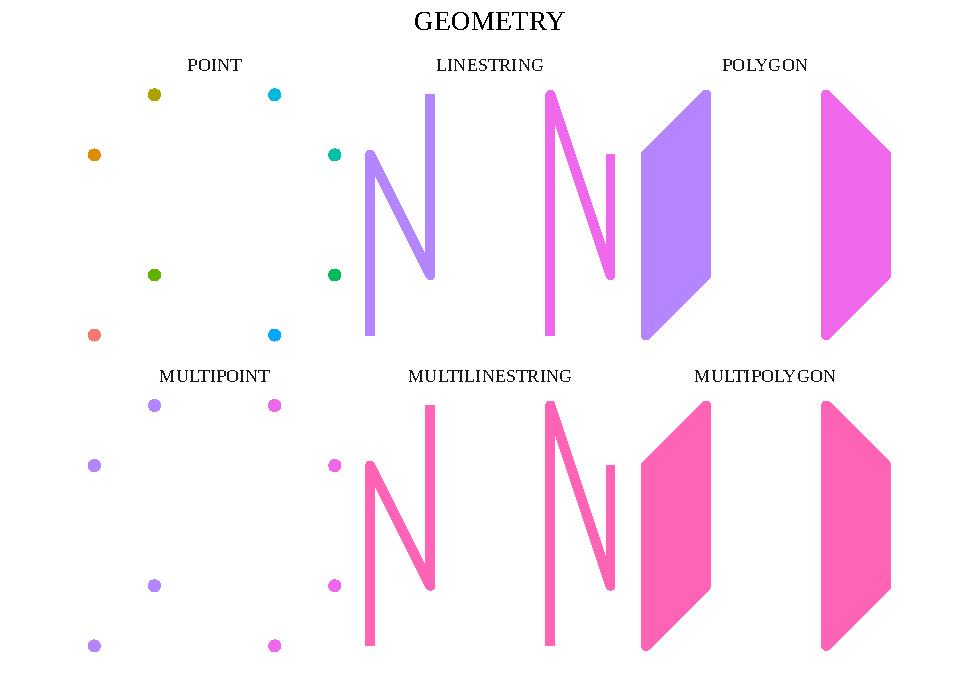
\includegraphics[width=1\linewidth]{3-spatial_files/figure-latex/unnamed-chunk-22-1} \end{center}

  \bibliography{book.bib}

\end{document}
